\documentclass{beamer}
\usepackage[utf8]{inputenc}
\usetheme{Madrid}
\usecolortheme{seahorse}
\setbeamertemplate{caption}[numbered]

\title{Series de Tiempo con Bosques Aleatorios (Random Forest)}
\author[iprea@udistrital.edu.co]{Wilson Eduardo Jeréz-Hernández}
\date{2 Diciembre de 2023}

\begin{document}
\frame{\titlepage}

\section{Series de Tiempo}

\begin{frame}
  \frametitle{Series de Tiempo}
  \begin{block}{Series de Tiempo}
  \begin{itemize}
      \item Una serie de tiempo es un conjunto de datos que se recopila o registra en intervalos regulares a lo largo del tiempo.
      \item Estas series pueden mostrar patrones complejos, tendencias a largo plazo y variaciones estacionales que las hacen adecuadas para una amplia gama de aplicaciones, desde la predicción financiera hasta el monitoreo de la salud.
  \end{itemize}
  \end{block}
\end{frame}
\begin{frame}
    \frametitle{Series de Tiempo}
      \begin{block}{Series de Tiempo}

	\begin{figure}
		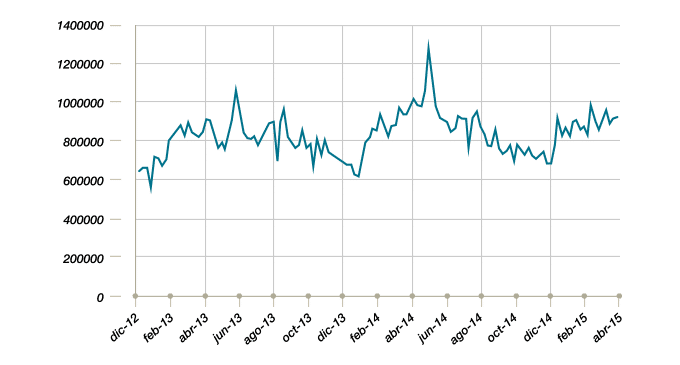
\includegraphics[width=0.7\textwidth]{grafico_ventas.png}
		\caption{https://www.pricing.cl/conocimiento/series-de-tiempo/}
	\end{figure}

  \end{block}
\end{frame}

\begin{frame}
\frametitle{Series de Tiempo}
\begin{block}{Características de una Serie de Tiempo}
\begin{enumerate}
    \item Movimientos a Largo Plazo o Tendencia.
    \item Movimientos Cíclicos: Fluctuaciones que ocurren en patrones recurrentes, pero no necesariamente a intervalos fijos.
    \item Movimientos Estacionales: Intervalos regulares a lo largo del tiempo.
    \item Movimientos Irregulares o Aleatorios.
\end{enumerate}
\end{block}

\end{frame}

\begin{frame}{Series de Tiempo}
    \begin{block}{Características de una Serie de Tiempo}
        \begin{figure}
            \centering
            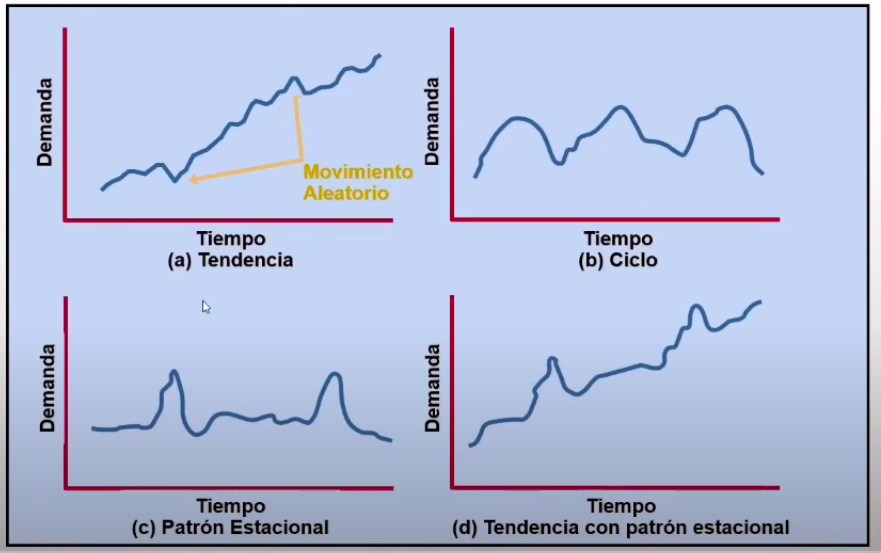
\includegraphics[width=0.5\textwidth]{Caracteristiucas.png}
            \caption{https://www.youtube.com/watch?app=desktop\&v=aUwXWGa8jK0}
        \end{figure}
    \end{block}
\end{frame}

\begin{frame}
  \frametitle{Tipos de Análisis en Series de Tiempo}
  Existen diferentes enfoques para analizar series de tiempo, dependiendo de los objetivos de la investigación. Los tres tipos principales de análisis son:
  \begin{enumerate}
    \item Análisis Descriptivo.
    \item Análisis Exploratorio/Inferencial.
    \item Análisis Predictivo.
  \end{enumerate}
\end{frame}

\begin{frame}
	\frametitle{Análisis Descriptivo.}
	\begin{enumerate}
		\item Este tipo de análisis tiene como objetivo comprender y describir las características fundamentales de una serie de tiempo.
		\item Proporciona una visión general de la tendencia, ciclos, estacionalidad y movimientos irregulares presentes en los datos.
		\item Ejemplos incluyen identificar patrones de comportamiento, calcular estadísticas descriptivas como promedios y desviaciones estándar, y visualizar la serie a través de gráficos.
	\end{enumerate}
\end{frame}

\begin{frame}
	\frametitle{Análisis Exploratorio/Inferencial.}
	\begin{enumerate}
		\item El análisis exploratorio profundiza en la identificación y comprensión de los factores subyacentes que influyen en el comportamiento de la serie de tiempo.
		\item Busca descubrir relaciones causa-efecto o correlaciones entre variables que puedan explicar patrones observados.
		\item Ejemplos incluyen el uso de técnicas estadísticas avanzadas, como el análisis de regresión, para modelar y comprender las relaciones entre variables.
	\end{enumerate}
\end{frame}

\begin{frame}
	\frametitle{Análisis Predictivo.}
	\begin{enumerate}
		\item El análisis predictivo utiliza datos históricos para hacer proyecciones sobre el comportamiento futuro de la serie de tiempo.
		\item Se basa en modelos y algoritmos de predicción que pueden prever valores futuros, tendencias y patrones.
		\item Ejemplos incluyen el uso de modelos de series de tiempo como ARIMA (Autoregressive Integrated Moving Average) y modelos de Machine Learning para predecir valores futuros de la serie.
	\end{enumerate}
\end{frame}

\begin{frame}
	\frametitle{Etapas Preliminares del Análisis}
	\begin{block}
		Antes de iniciar el análisis de una serie de tiempo, es esencial llevar a cabo una serie de etapas preliminares que establecen las bases para un estudio efectivo:
		\begin{itemize}
			\item \textbf{Experticia en el Ámbito de Aplicación.} 
			\item \textbf{Definición de Objetivos.}
			\item \textbf{Recolección de Datos.}
			\item \textbf{Análisis Exploratorio.} 
			\item \textbf{Representación de Componentes.}
		\end{itemize}
	\end{block}
  \end{frame}
  
  \begin{frame}
	\frametitle{Estacionariedad y Función de Autocorrelación}
	Muchos métodos estadísticos para el análisis de series de tiempo requieren, como paso previo, verificar la estacionariedad de la señal. La estacionariedad se refiere a que las propiedades estadísticas de la serie se mantienen constantes a lo largo del tiempo.
	
	La función de autocorrelación es una herramienta esencial en este contexto, ya que permite comparar la señal con ella misma y revelar información valiosa sobre la estructura temporal de la serie.
  \end{frame}
  
  \begin{frame}
	\frametitle{Pre-procesamiento de la Serie de Tiempo}
	\begin{enumerate}
	  \item \textbf{Manejo de Datos Faltantes:} 
	  \item \textbf{Uniformización del Espaciamiento Temporal.}
	  \item \textbf{Manejo de Valores Extremos.}
	  \item \textbf{Elección del Horizonte de Tiempo.}
	  \item \textbf{Partición de los Datos (Solo para Análisis Predictivo).}
	\end{enumerate}
	El pre-procesamiento de la serie de tiempo es esencial para garantizar que los datos estén listos para el análisis posterior y para obtener resultados confiables y significativos en función de los objetivos establecidos.
  \end{frame}
  


\section{Machine Learning}
	
\begin{frame}
	\frametitle{Modelo de Aprendizaje de Máquina}
					\begin{block}{Modelo vs Algoritmo}	
	\begin{itemize}
		\item \textbf{¿Qué es un modelo?} \textit{Un modelo es cualquier tipo de función que tiene capacidad predictiva.}
		\item\textbf{¿Qué es un algoritmo?}\textit{Un algoritmo es un conjunto de pasos realizados en orden  con el objetivo de realizar una tarea o resolver un problema específico.}
		\item Un \textbf{Modelo de Aprendizaje de Máquina} es el resultado del proceso de entrenar un algoritmo con un conjunto de datos.
	\end{itemize}
\end{block}
\end{frame}
	
	
\begin{frame}
\frametitle{Modelo de Aprendizaje de Máquina}
\textit{\textbf{``Todos los modelos son erroneos, pero algunos son útiles."}}
\begin{figure}
	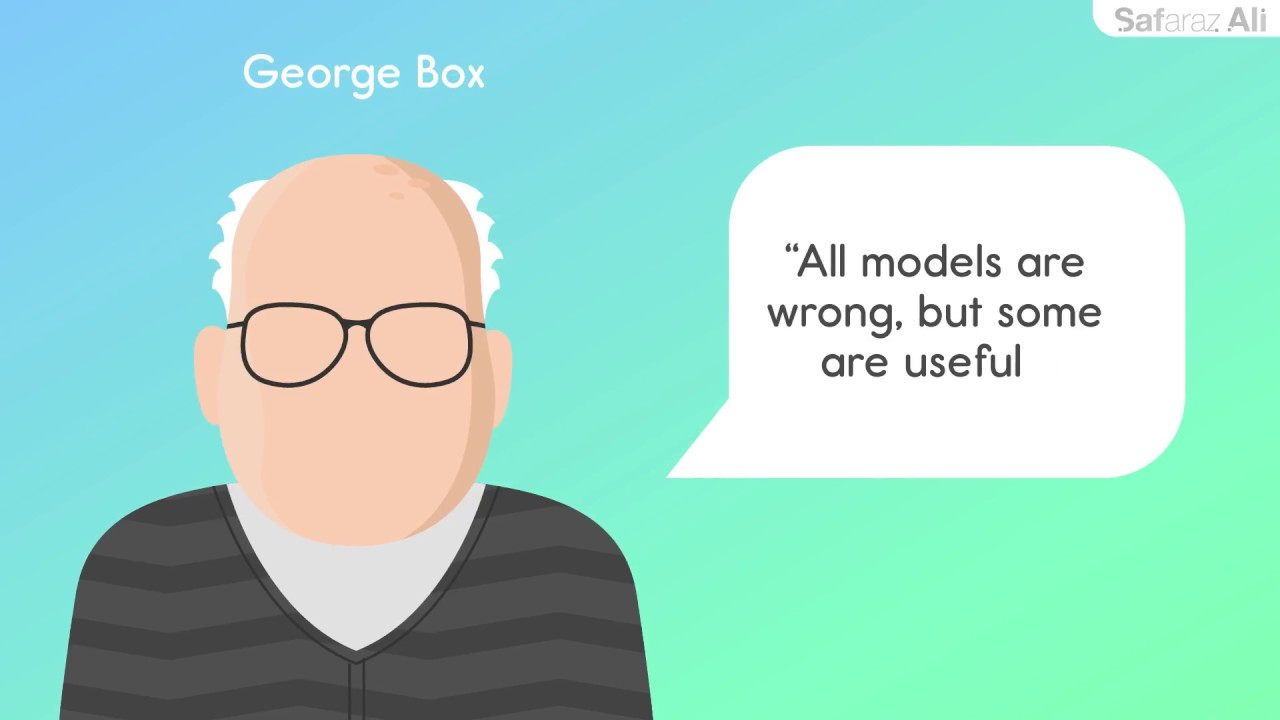
\includegraphics[width=0.7\textwidth]{Box_imagen.jpg}
	\caption{https://www.youtube.com/@SafarazAli}
\end{figure}
\end{frame}

 	
	
\begin{frame}
\frametitle{Modelo de Aprendizaje de Máquina}
\textit{\textbf{``La verdad es demasiado complicada como para permitir algo más que una aproximación."}}
\begin{figure}
	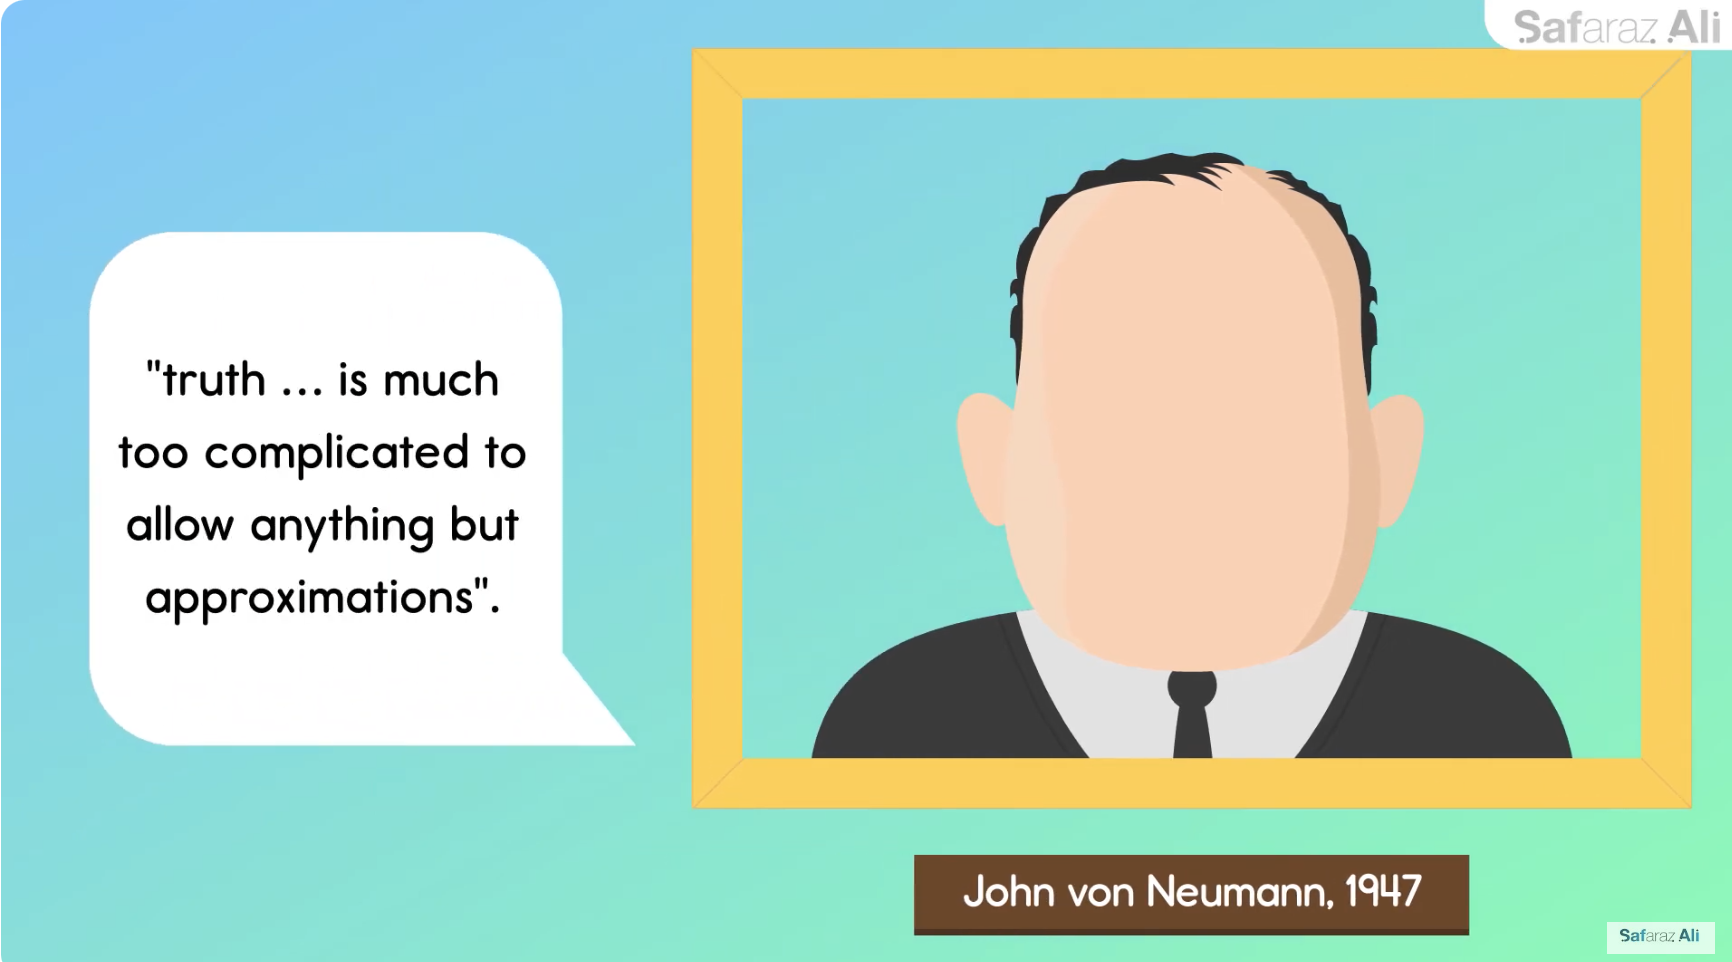
\includegraphics[width=0.7\textwidth]{Von_Newman_imagen}
	\caption{https://www.youtube.com/@SafarazAli}
\end{figure}
\end{frame}
	
	
\begin{frame}
	\frametitle{En Resumen}
	\begin{itemize}
		\item El \textbf{algoritmo} es como las instrucciones para construir una máquina de predicción.
		\item El \textbf{modelo} es la máquina ya construida y entrenada para realizar una tarea específica.
	\end{itemize}
\end{frame}
	

	

\begin{frame}{Modelos de Aprendizaje de Máquina}
\begin{block}{El Problema}
	\begin{figure}
		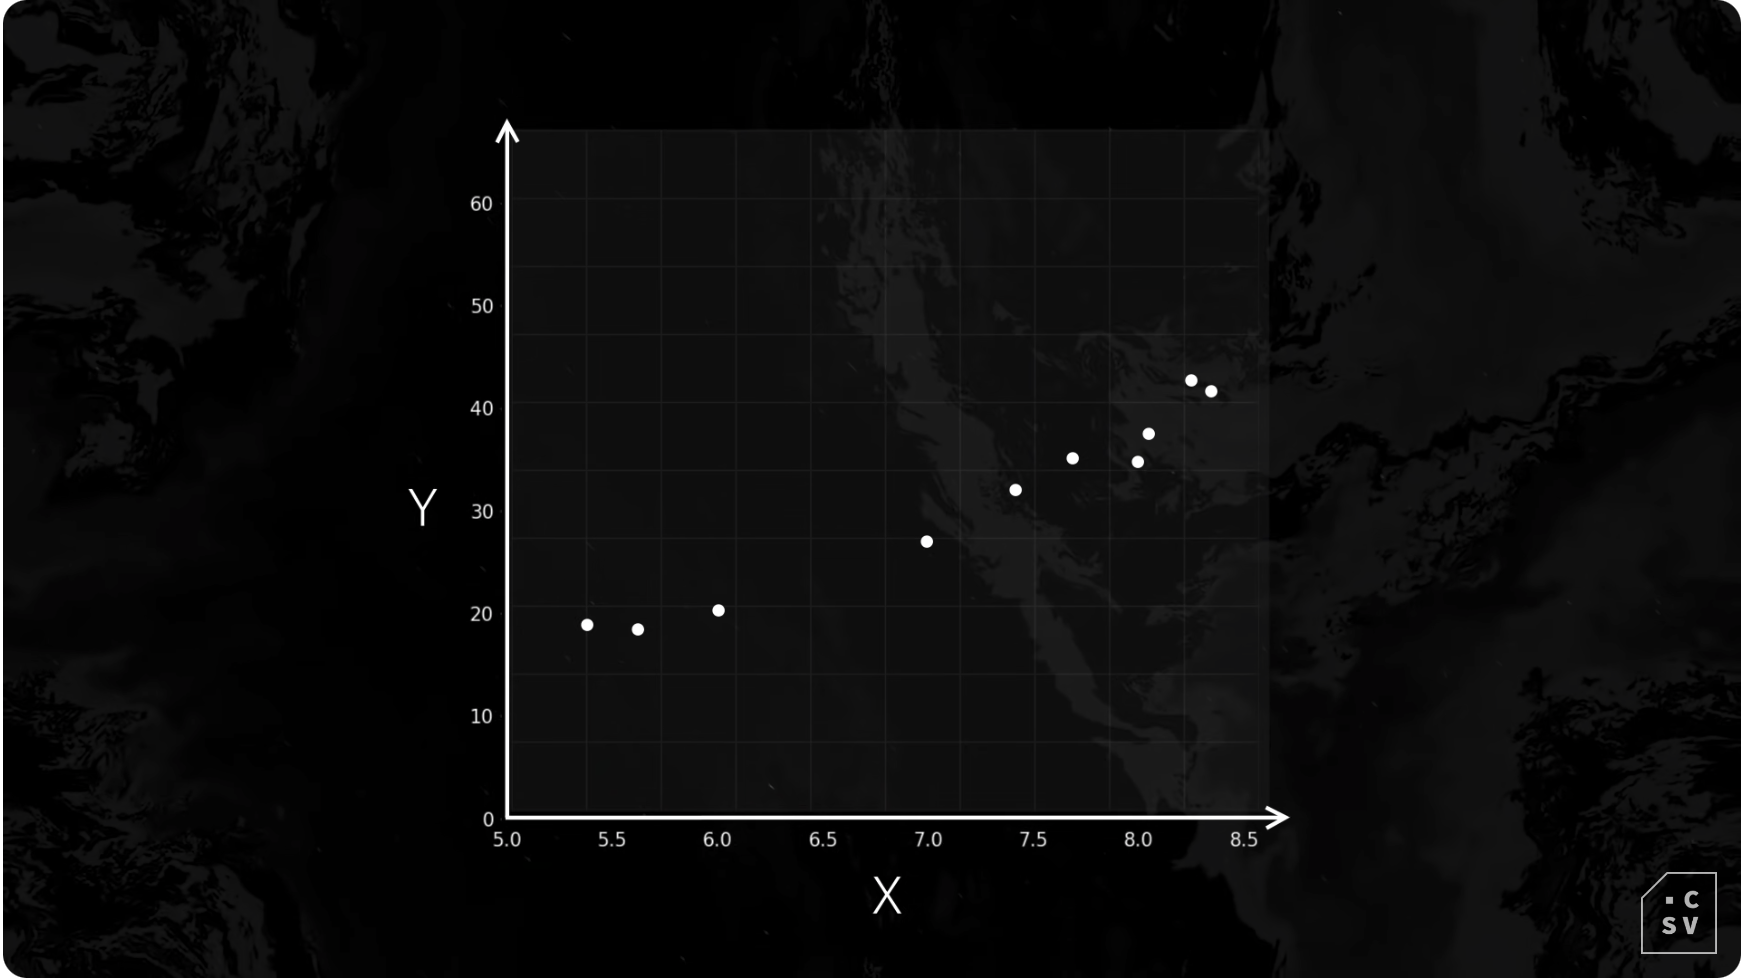
\includegraphics[width=0.7\textwidth]{modelo-algoritmo_1}
		\caption{https://www.youtube.com/}
		\centering
	\end{figure}
\end{block}
		
\end{frame}
	
\begin{frame}{Modelos de Aprendizaje de Máquina}
\begin{block}{El Modelo}
	\begin{figure}
		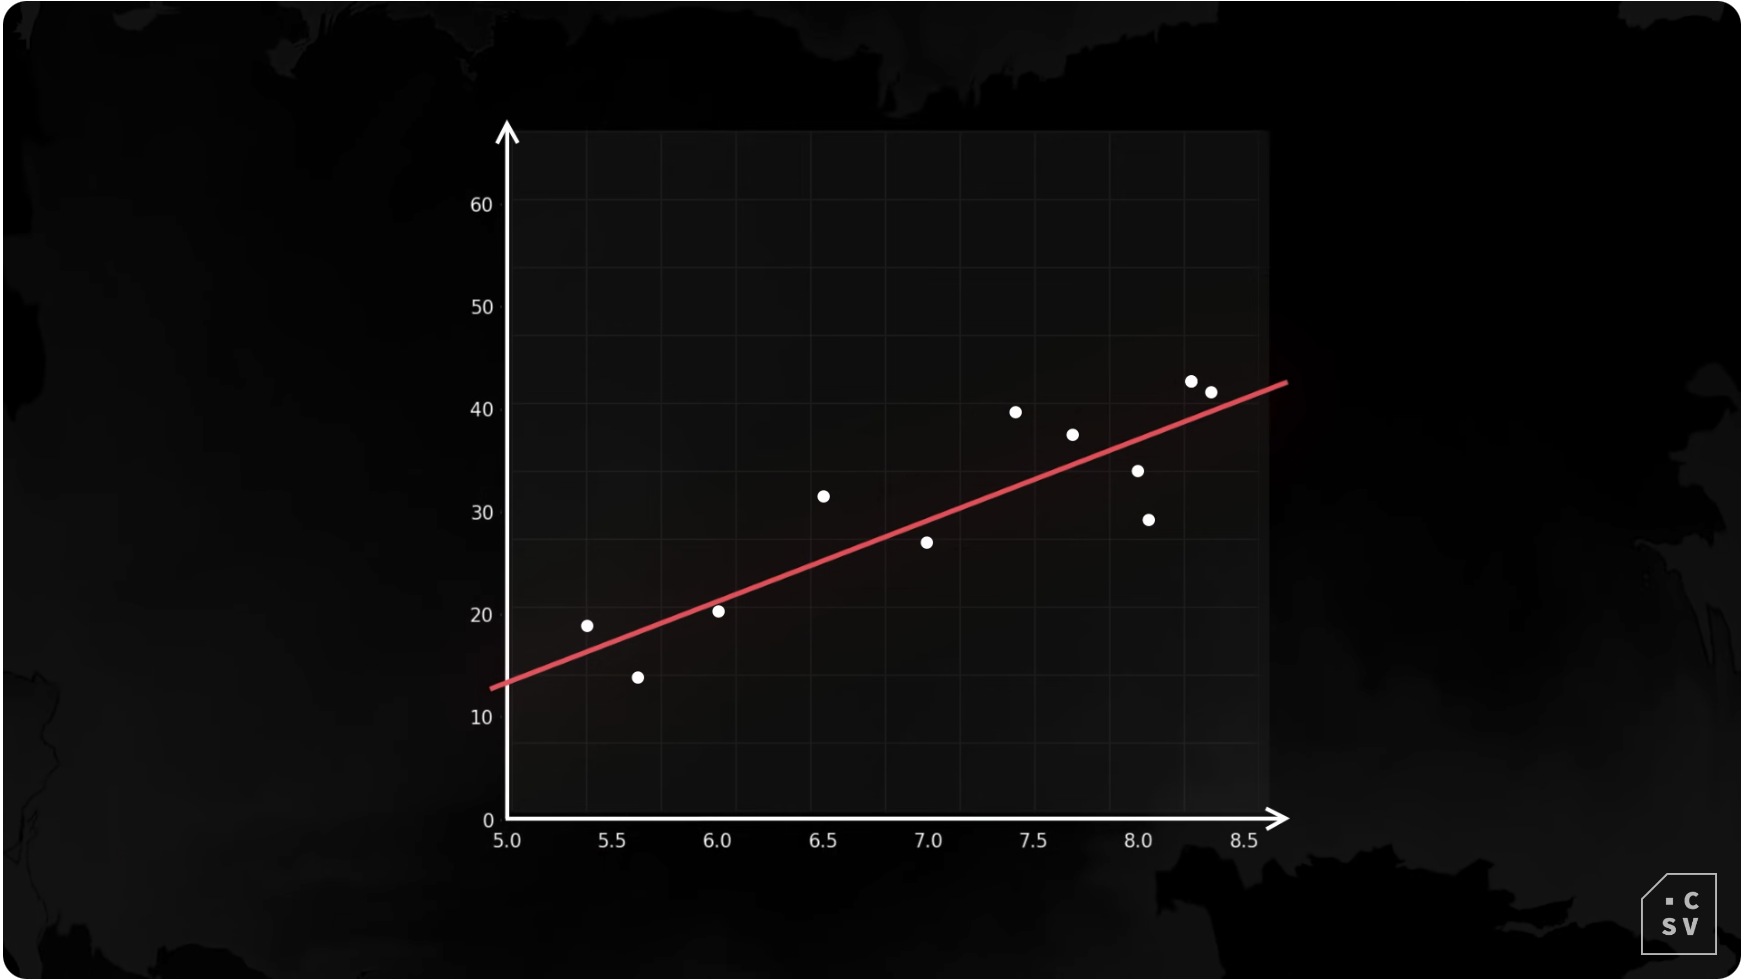
\includegraphics[width=0.7\textwidth]{modelo-algoritmo_2}
		\caption{https://www.youtube.com/}
		\centering
	\end{figure}
\end{block}
		
\end{frame}
	
\begin{frame}{Modelos de Aprendizaje de Máquina}
\begin{block}{El Algoritmo}
	\begin{figure}
		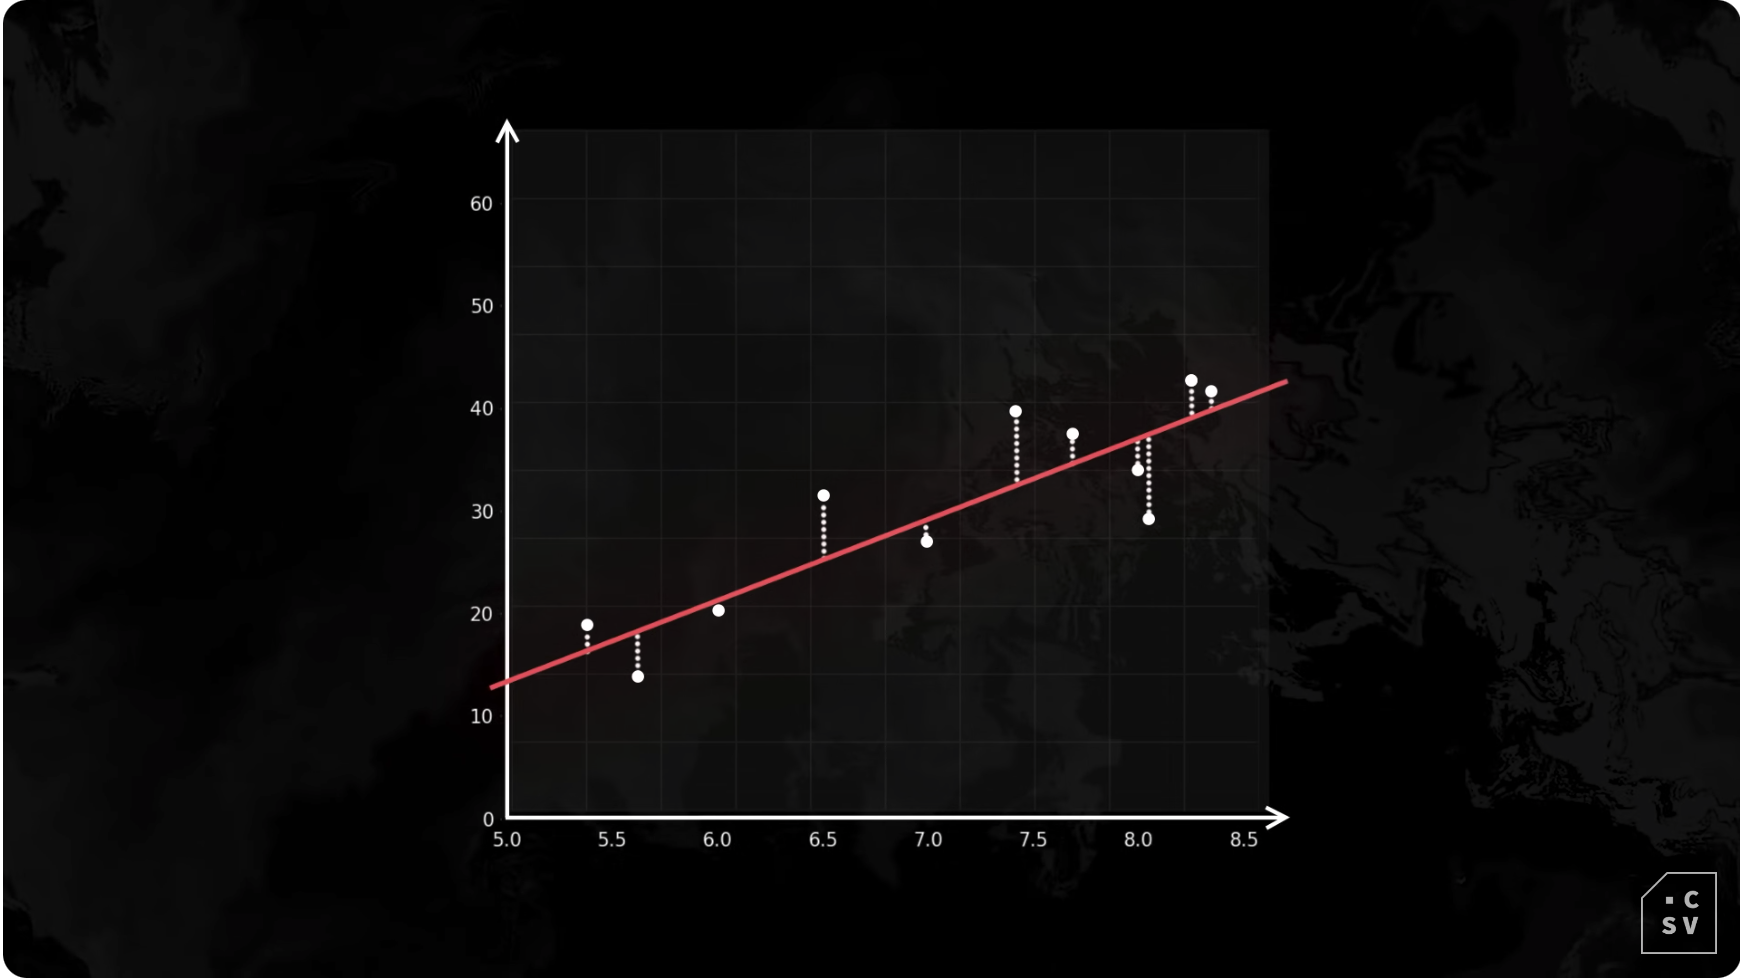
\includegraphics[width=0.7\textwidth]{modelo-algoritmo_3}
		\caption{https://www.youtube.com/}
		\centering
	\end{figure}
\end{block}

\end{frame}

	

\begin{frame}
	\frametitle{Conceptos en Aprendizaje de Máquina}
			\begin{block}{El Conjunto de Datos}
	\begin{itemize}
		\item \textbf{Características (Features)}:
		\begin{itemize}
			\item Representan las entradas o datos de entrada en un modelo de Machine Learning.
			\item Son las variables o atributos que se utilizan para hacer predicciones.
			\item Ejemplos: píxeles de una imagen, palabras en un documento, mediciones en un conjunto de datos.
		\end{itemize}			
		\item \textbf{Etiquetas (Labels)}:
		\begin{itemize}
			\item Representan las salidas o resultados deseados en un modelo de Machine Learning.
			\item Son las respuestas que el modelo debe aprender a predecir.
			\item Ejemplos: categorías de imágenes (perro, gato), clasificación de texto (positivo, negativo), valor numérico de una propiedad.
		\end{itemize}
		\item \textbf{Ejemplos (Examples)}: son instancias de datos utilizadas para entrenar y evaluar modelos de aprendizaje automático.
	\end{itemize}
		\end{block}
\end{frame}


\begin{frame}
\frametitle{Conceptos en Aprendizaje de Máquina}
\begin{figure}
	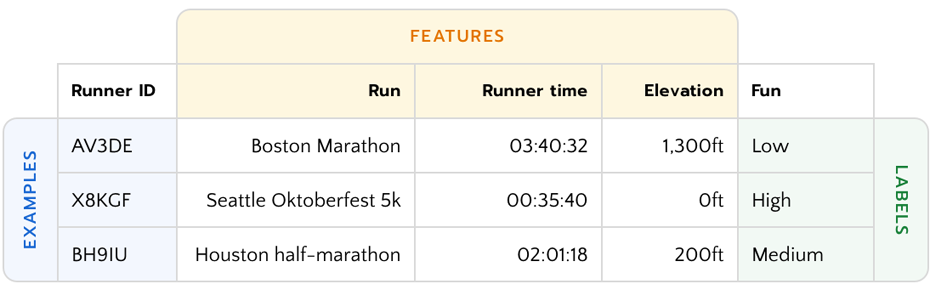
\includegraphics[width=0.9\textwidth]{labels_features}
	\caption{https://pair.withgoogle.com/chapter/data-collection/}
	\centering
\end{figure}
\begin{block}{}
El dataframe anterior contiene datos sobre carreras que una aplicación podría usar para entrenar un modelo de aprendizaje automático para predecir qué tan divertida será una carrera determinada.
\end{block}
\end{frame}

\begin{frame}
\frametitle{Conceptos en Aprendizaje de Máquina}
	\begin{block}{}
\begin{figure}
	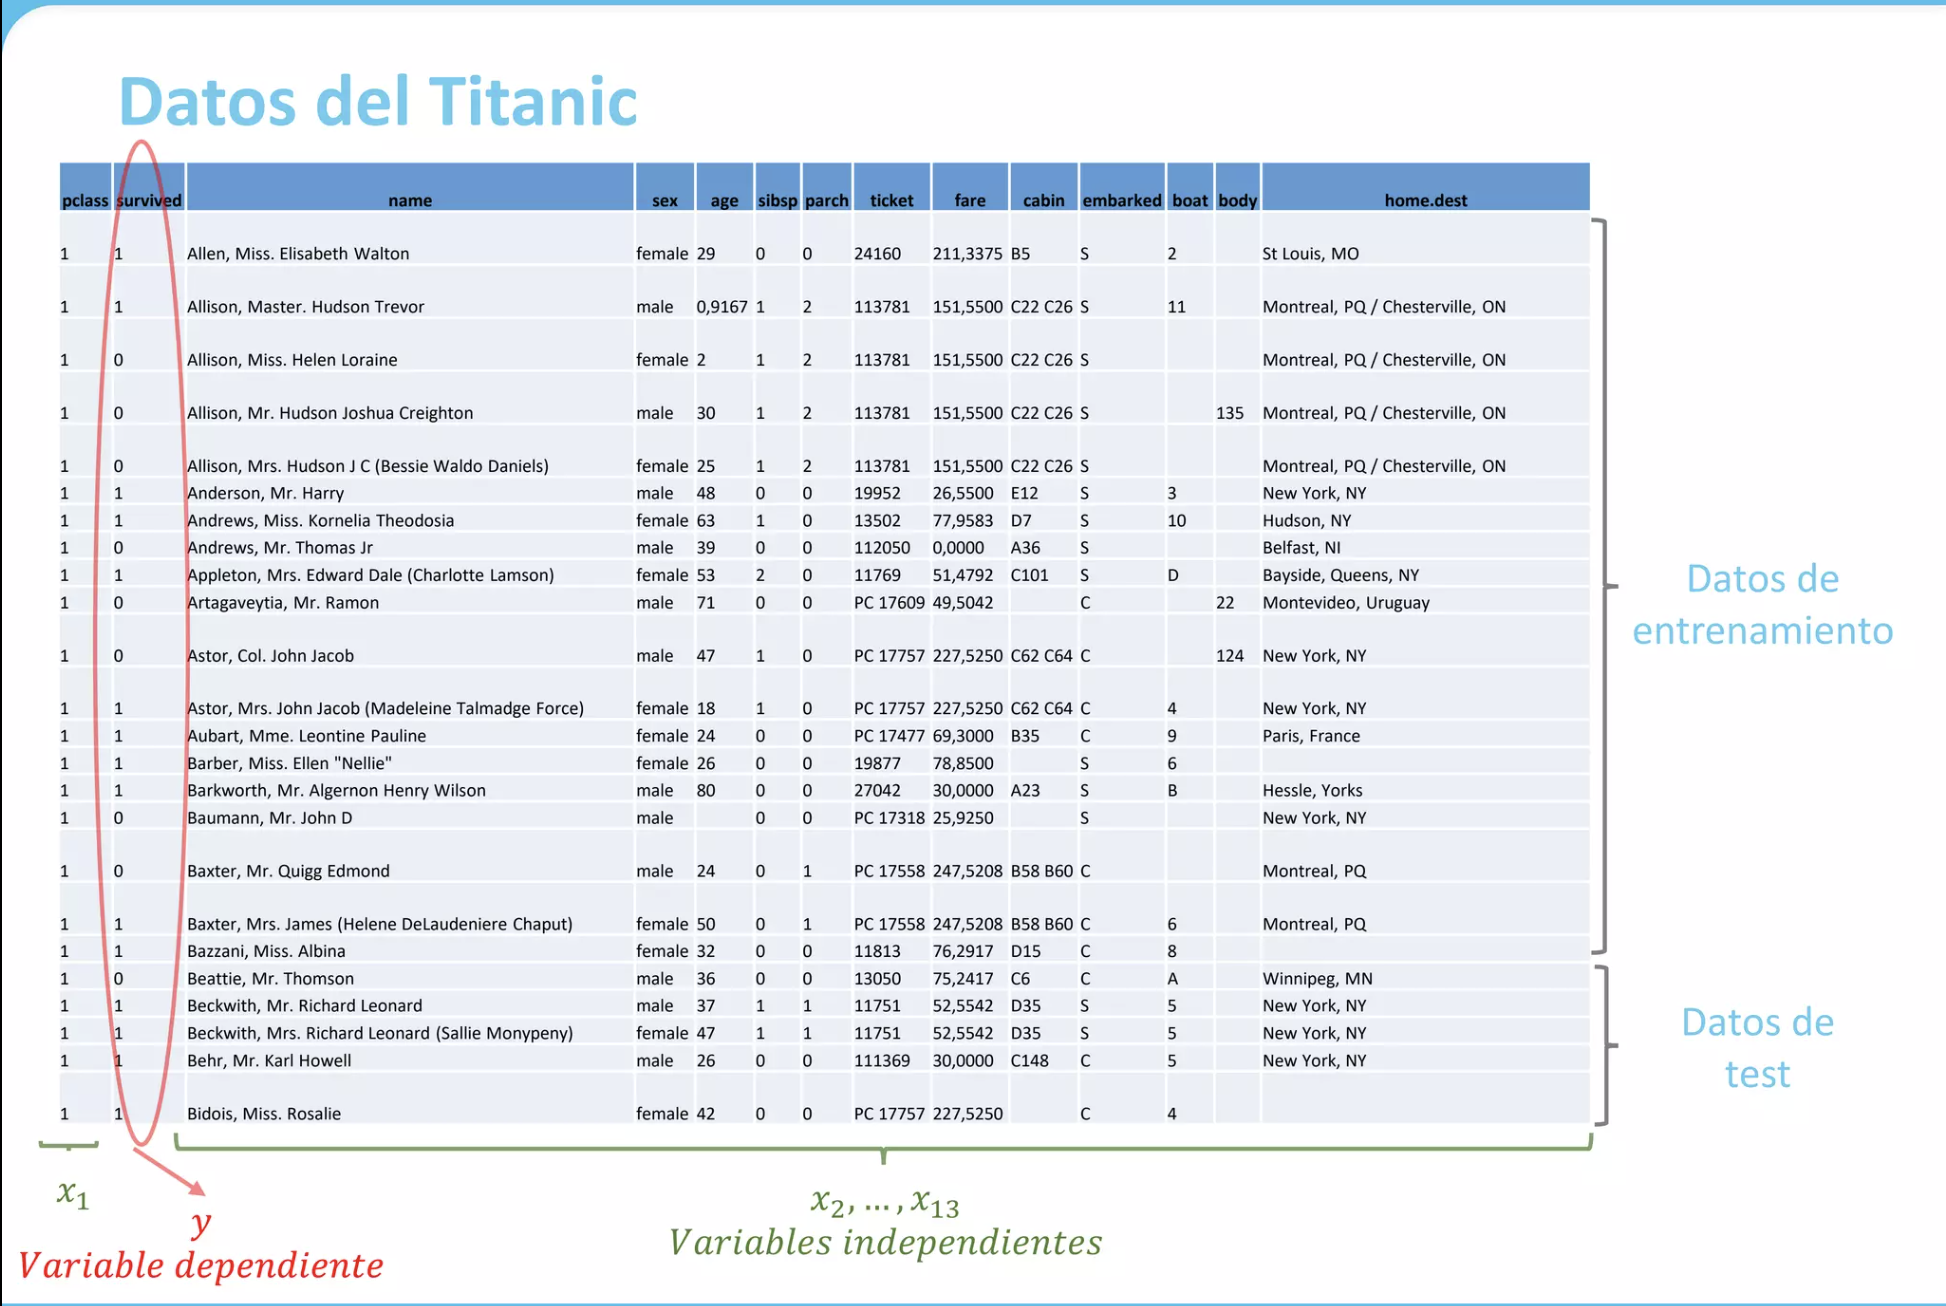
\includegraphics[width=0.7\textwidth]{Titanic}
	\caption{https://es.slideshare.net/JavierEsteveMeli/}
	\centering
\end{figure}
\end{block}
\end{frame}


\begin{frame}
	\frametitle{Conceptos en Aprendizaje de Máquina}
		\begin{block}{Categorias}
	
	\begin{itemize}
		\item \textbf{Machine Learning Supervisado}:
		\begin{itemize}
			\item Entrenado con datos que especifican tanto la entrada como la salida.
			\item Por ejemplo, imágenes de números escritos a mano etiquetados con los números correspondientes.
			\item Reconoce patrones y relaciones entre las características y las etiquetas conocidas.
		\end{itemize}
		
		\item \textbf{Machine Learning No Supervisado}:
		\begin{itemize}
			\item Entrenado con datos sin etiquetar.
			\item Analiza datos para encontrar patrones o conexiones significativas.
			\item Agrupa datos en categorías o encuentra estructuras ocultas.
			\item Ejemplo: agrupación de noticias en categorías como deportes o crímenes.
		\end{itemize}
	\end{itemize}
		\end{block}
\end{frame}

\begin{frame}
	\frametitle{Conceptos en Aprendizaje de Máquina}
\begin{block}{Categorías principales del Aprendizaje de Máquina}	
\begin{figure}
	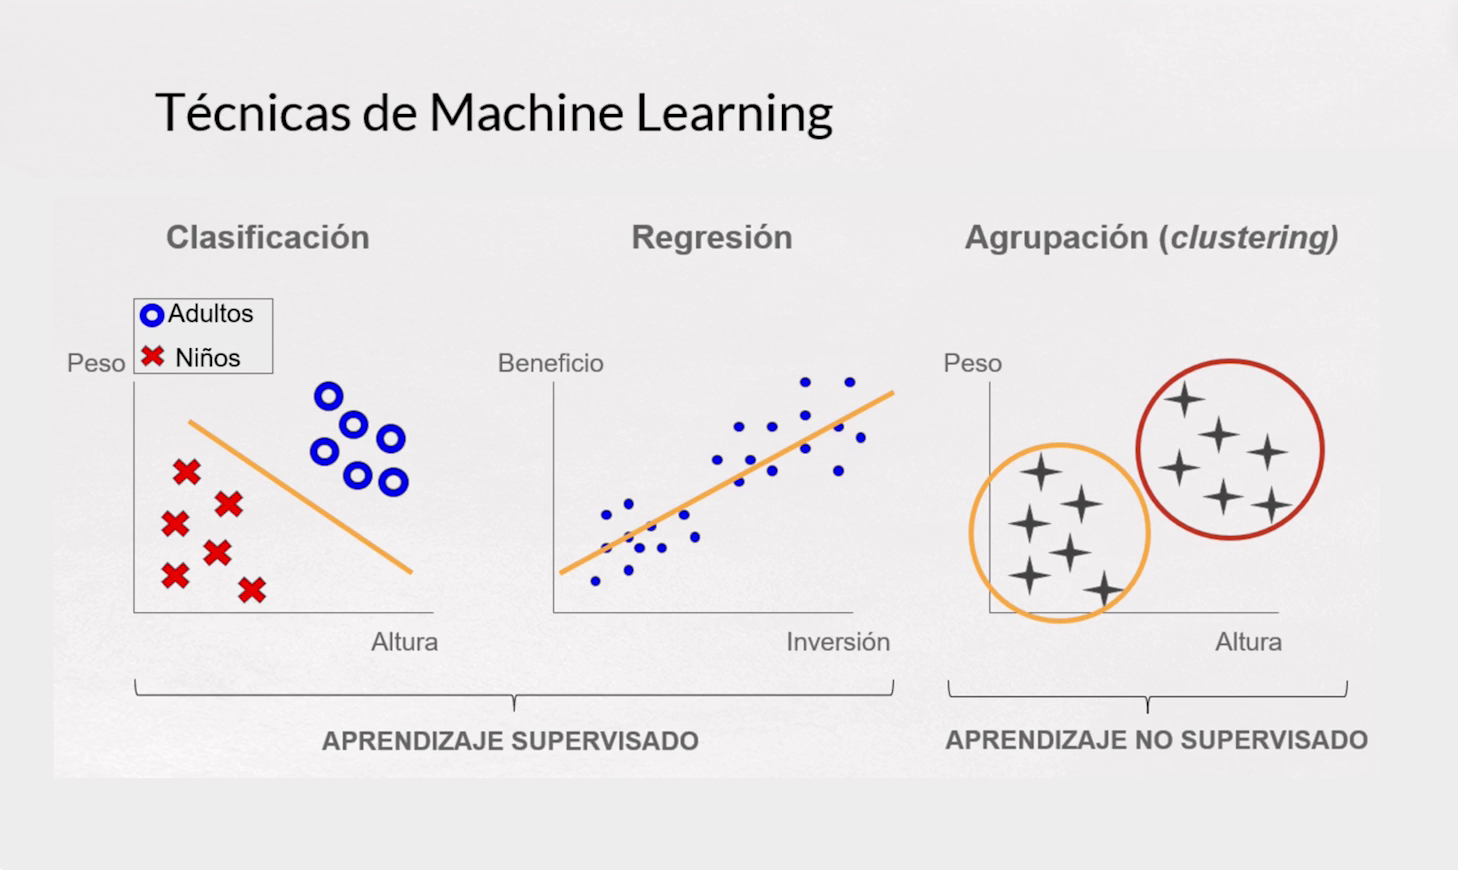
\includegraphics[width=0.9\textwidth]{supervisado_nosupervisado.png}
	\caption{https://openwebinars.net/blog/modelos-de-machine-learning/}
\end{figure}
\end{block}
\end{frame}



\begin{frame}
	\frametitle{Tipos de Modelos en Aprendizaje de Máquina}
	
	\begin{block}{Modelos Supervisados}
	\begin{itemize}
		\item Regresión lineal
		\item Regresión logística
		\item Máquinas de soporte vectorial (SVM)
		\item Árboles de decisión
		\item Redes neuronales
	\end{itemize}
\end{block}

\end{frame}

	
\begin{frame}
	\frametitle{Tipos de Modelos en Aprendizaje de Máquina}
		\begin{block}{Modelos No Supervisados}
	\begin{itemize}
		\item K-Means (clustering)
		\item Análisis de Componentes Principales (PCA)
		\item Redes Generativas Adversariales (GANs)
		\item Reglas de asociación
		\item Detección de anomalías
	\end{itemize}
\end{block}
\end{frame}
	
\begin{frame}
	\frametitle{Los Datos en el Aprendizaje de Máquina}
	\begin{block}{Partición de la Data}	
		\begin{figure}
			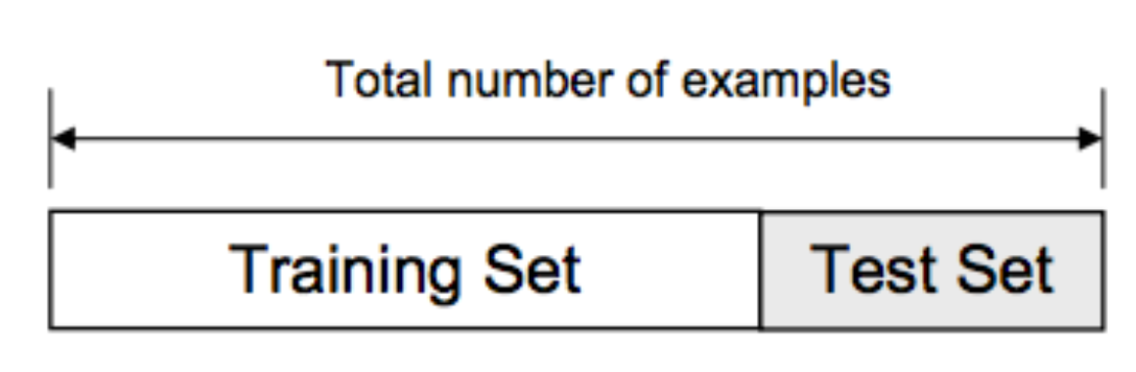
\includegraphics[width=0.7\textwidth]{entrenamiento_prueba}
			\caption{http://exponentis.es/como-dividir-un-conjunto-de-entrenamiento-en-dos-partes-train-test-split}
		\end{figure}
	\end{block}
\end{frame}
	
	
	
\begin{frame}
	\frametitle{Partición de la Data}
			\begin{block}{Partición de la Data}	
	\begin{itemize}
	\item  \textbf{Conjunto de Entrenamiento:} 
	Este conjunto se utiliza para entrenar el modelo. Contiene una parte significativa de los datos y es donde el algoritmo de aprendizaje automático "aprende" a partir de las observaciones. El modelo ajusta sus parámetros utilizando este conjunto de datos.
	\item \textbf{ Conjunto de Prueba:} 
	Este conjunto se utiliza para evaluar el rendimiento del modelo una vez que ha sido entrenado. Contiene datos que el modelo no ha visto durante el proceso de entrenamiento. Se utiliza para simular cómo el modelo se comportaría en la práctica al hacer predicciones en datos no vistos.
		\end{itemize}
			\end{block}
\end{frame}

\begin{frame}
	\frametitle{Función de Costo en Modelos}
			\begin{block}{Función de Costo en modelos supervisados}	
	\begin{itemize}
		\item También conocida como función de pérdida o función de error.
		\item Mide qué tan bien se hacen las predicciones del modelo en comparación con los valores reales en el conjunto de entrenamiento.
	\end{itemize}
		\end{block}
\end{frame}

\begin{frame}
	\frametitle{Función de Costo}
	\begin{block}{Función de Costo en Modelos Supervisados}	
		\begin{figure}
	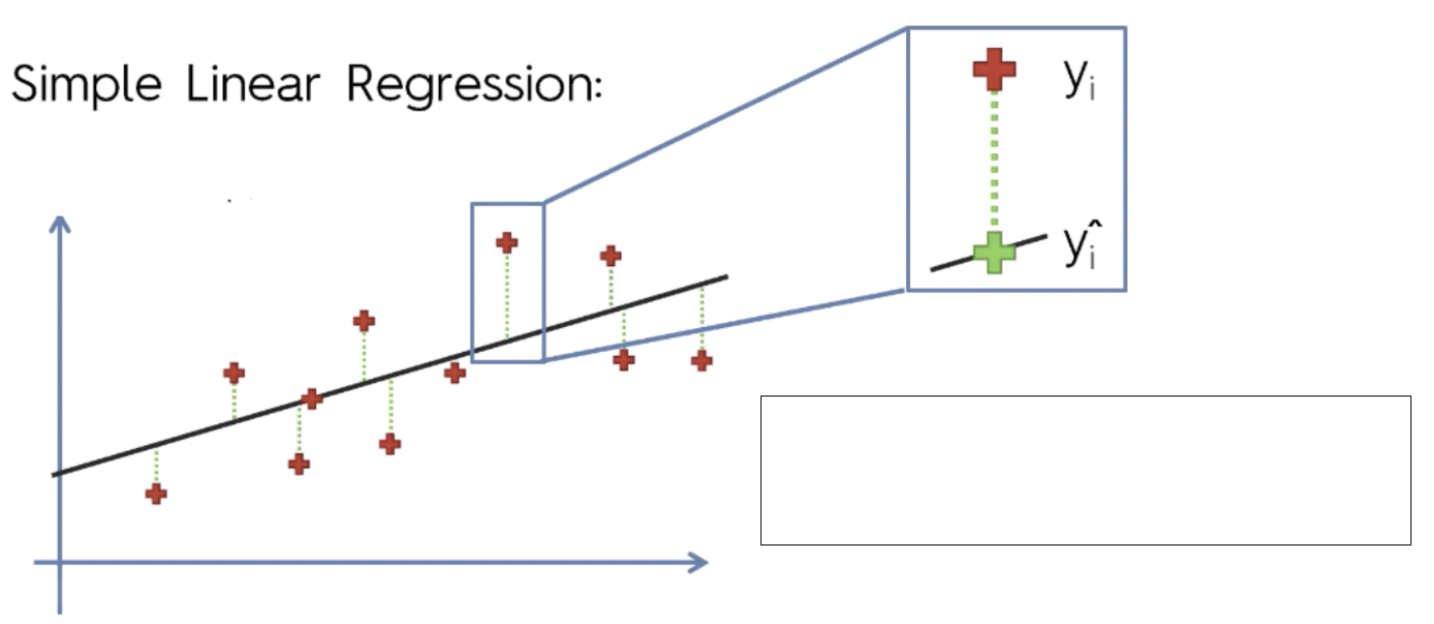
\includegraphics[width=0.9\textwidth]{funcion_coste}
	\caption{https://www.themachinelearners.com/}
\end{figure}
	\end{block}
\end{frame}

\begin{frame}
	\frametitle{Evaluación del Error}
		\begin{block}{Función de Costo en Modelos Supervisados}	
	\begin{itemize}
		\item La función de costo cuantifica la discrepancia entre las predicciones del modelo y los valores reales.
		\item Evalúa la calidad de las predicciones en el conjunto de entrenamiento.
				\item Durante el proceso de entrenamiento, la función de costo se utiliza para ajustar los parámetros del modelo.
		\item El objetivo es encontrar los valores de parámetros que minimizan la función de costo.
	\end{itemize}
		\end{block}
\end{frame}




\begin{frame}
	\frametitle{Funciones de Costo}
			\begin{block}{Función de Costo en Modelos Supervisados}	
				La elección de la función de costo depende del tipo de problema de Machine Learning:
	\begin{itemize}
		\item \textbf{MSE (Mean Squared Error)}: Utilizado en problemas de regresión.
		\item \textbf{Entropía Cruzada (Cross-Entropy)}: Utilizado en problemas de clasificación.
	\end{itemize}
	\end{block}
\end{frame}

\begin{frame}
	\frametitle{Función de Costo}
			\begin{block}{Función de Costo en Modelos No Supervisados}	
	\begin{itemize}
		\item En modelos no supervisados, también se utilizan funciones de costo.
		\item Estas funciones miden la calidad de las soluciones o guían el proceso de aprendizaje no supervisado.
	\end{itemize}
		\end{block}
\end{frame}

\begin{frame}
	\frametitle{Función de Costo}
		\begin{block}{Función de Costo en Modelos No Supervisados}	
	\begin{itemize}
		\item En K-Medias (Clustering), se utiliza la función de costo \textbf{``inercia"} o \textbf{``SSE"} para minimizar la distancia de las instancias a los centroides.
			\item Aunque \textbf{PCA} no se ajusta en el sentido tradicional, busca una solución que\textbf{ optimice la varianza }de las proyecciones de datos.
	\end{itemize}
	\end{block}
\end{frame}

\section{Random Forest}

\begin{frame}
    \frametitle{Random Forest}
\begin{block}{Árboles de Decisión}
      Los árboles de decisión son algoritmos versátiles utilizados en tareas de clasificación y regresión. Son especialmente útiles para capturar relaciones no lineales en los datos y son una excelente opción para principiantes en el campo del Machine Learning.
\end{block}
  

\end{frame}

\begin{frame}
\frametitle{Random Forest}
  \begin{block}{Bootstrap Aggregation (Bagging)}
      El algoritmo Bagging se utiliza para mejorar la estabilidad y precisión de los modelos, incluyendo árboles de decisión. A través de la combinación de múltiples modelos entrenados con muestras de datos seleccionadas con reemplazo, Bagging reduce la varianza y aumenta la precisión.
  \end{block} 
  
\end{frame}

\begin{frame}

  \frametitle{Random Forest}
  \begin{block}{Bosques Aleatorios (Random Forest)}
        Bosques Aleatorios son una extensión de Bagging que combina múltiples árboles de decisión mediante la aleatorización de características. Esto produce un modelo robusto y de alto rendimiento que es eficaz en la clasificación y la regresión de series de tiempo.
  \end{block}

\end{frame}


\section{REDUCCIÓN DE DIMENSIONALIDAD}

\begin{frame}
	\frametitle{MODELOS DE APRENDIZAJE DE MÁQUINA}
	\begin{block}{}	
		\center
		\textbf{ANÁLISIS DE COMPONENTES PRINCIPALES}
	\end{block}
\end{frame}

\begin{frame}
	\frametitle{REDUCCIÓN DE DIMENSIONALIDAD}
	\begin{block}{Análisis de Componentes Principales}	
		\begin{figure}
			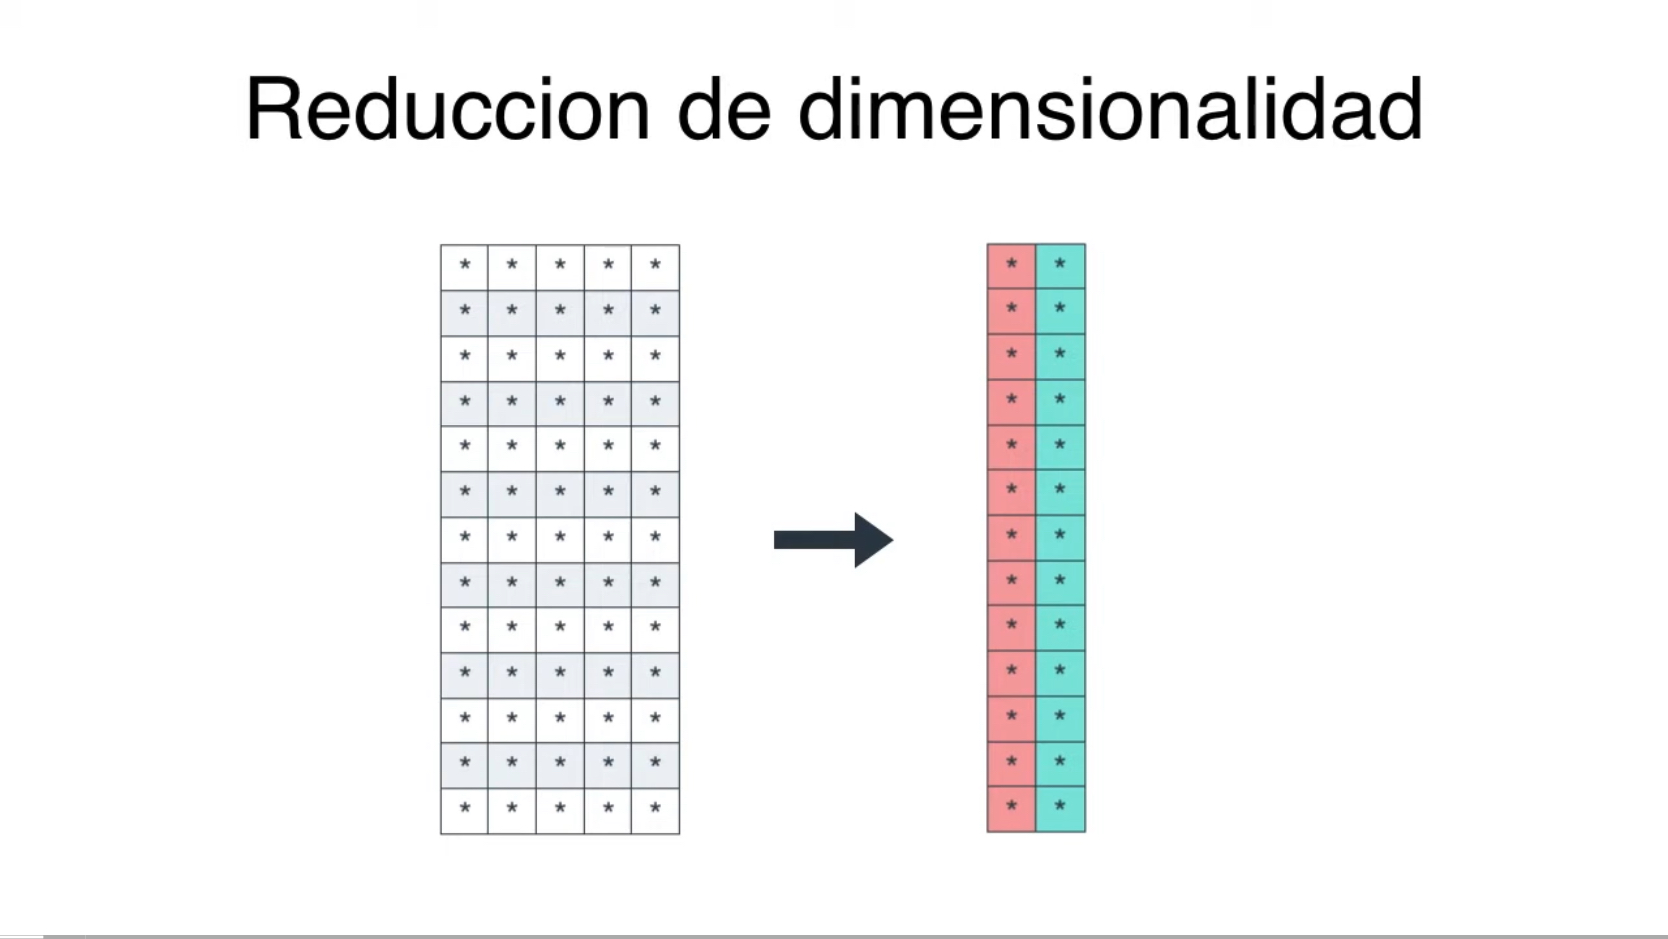
\includegraphics[width=0.9\textwidth]{PCA/IMG_3525.jpg}
			\caption{https://serrano.academy/espanol/}
		\end{figure}
	\end{block}
\end{frame}

\begin{frame}
\frametitle{REDUCCIÓN DE DIMENSIONALIDAD}
\begin{block}{Análisis de Componentes Principales}	
	\begin{figure}
		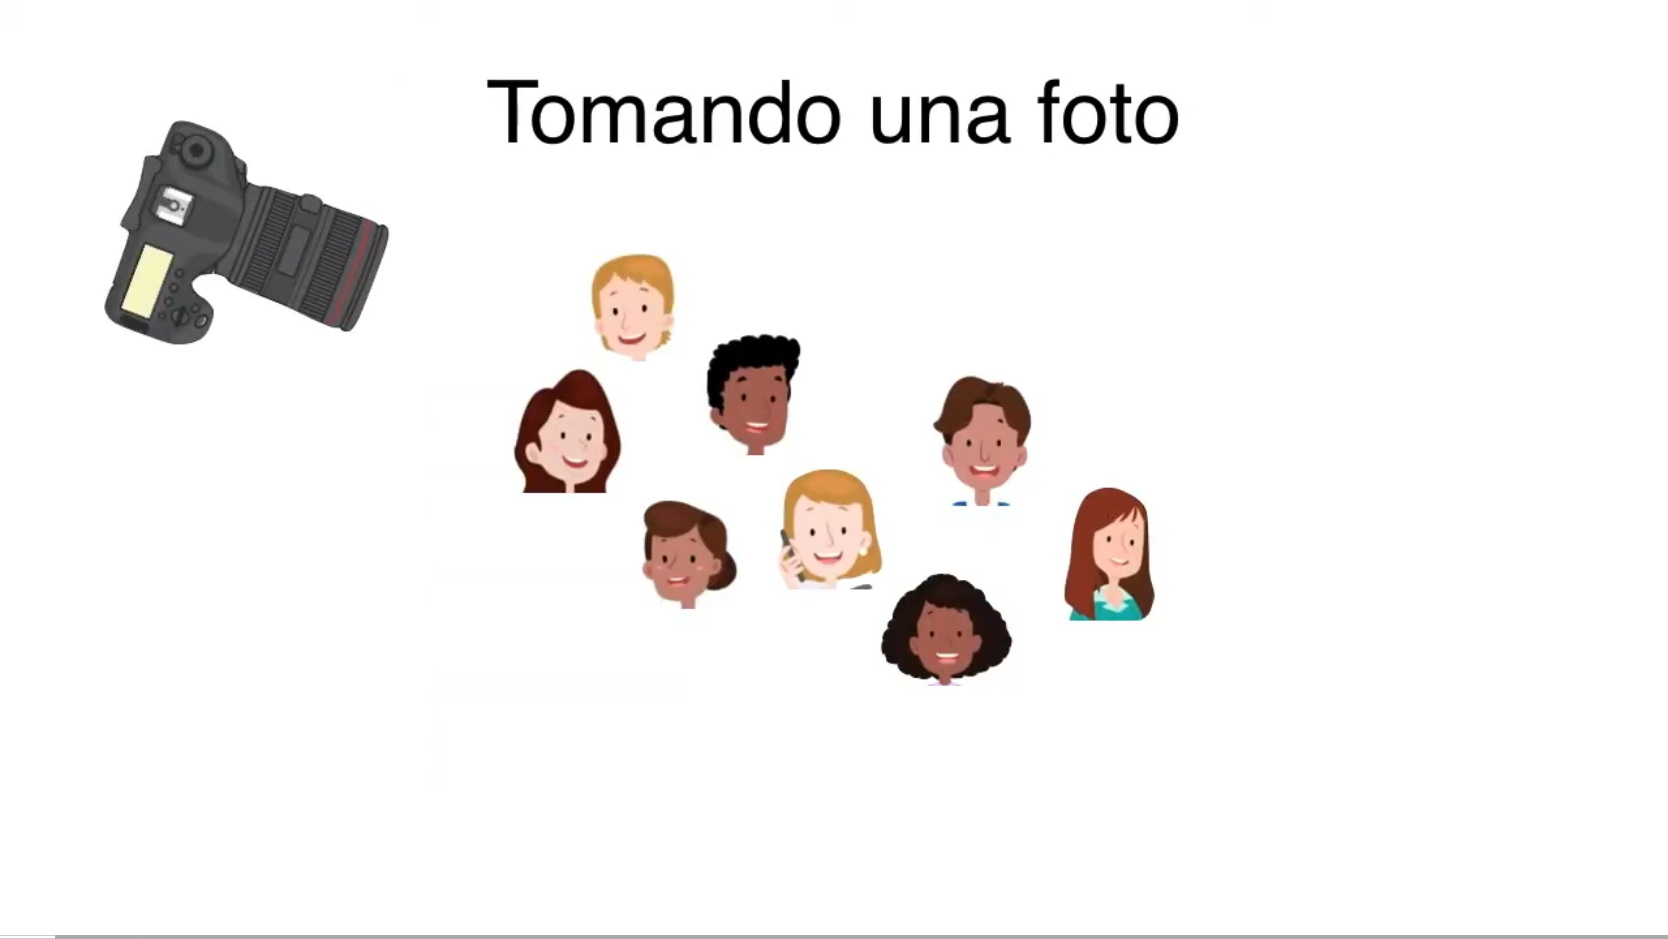
\includegraphics[width=0.9\textwidth]{PCA/IMG_3526.jpg}
		\caption{https://serrano.academy/espanol/}
	\end{figure}
\end{block}
\end{frame}

\begin{frame}
\frametitle{REDUCCIÓN DE DIMENSIONALIDAD}
\begin{block}{Análisis de Componentes Principales}	
	\begin{figure}
		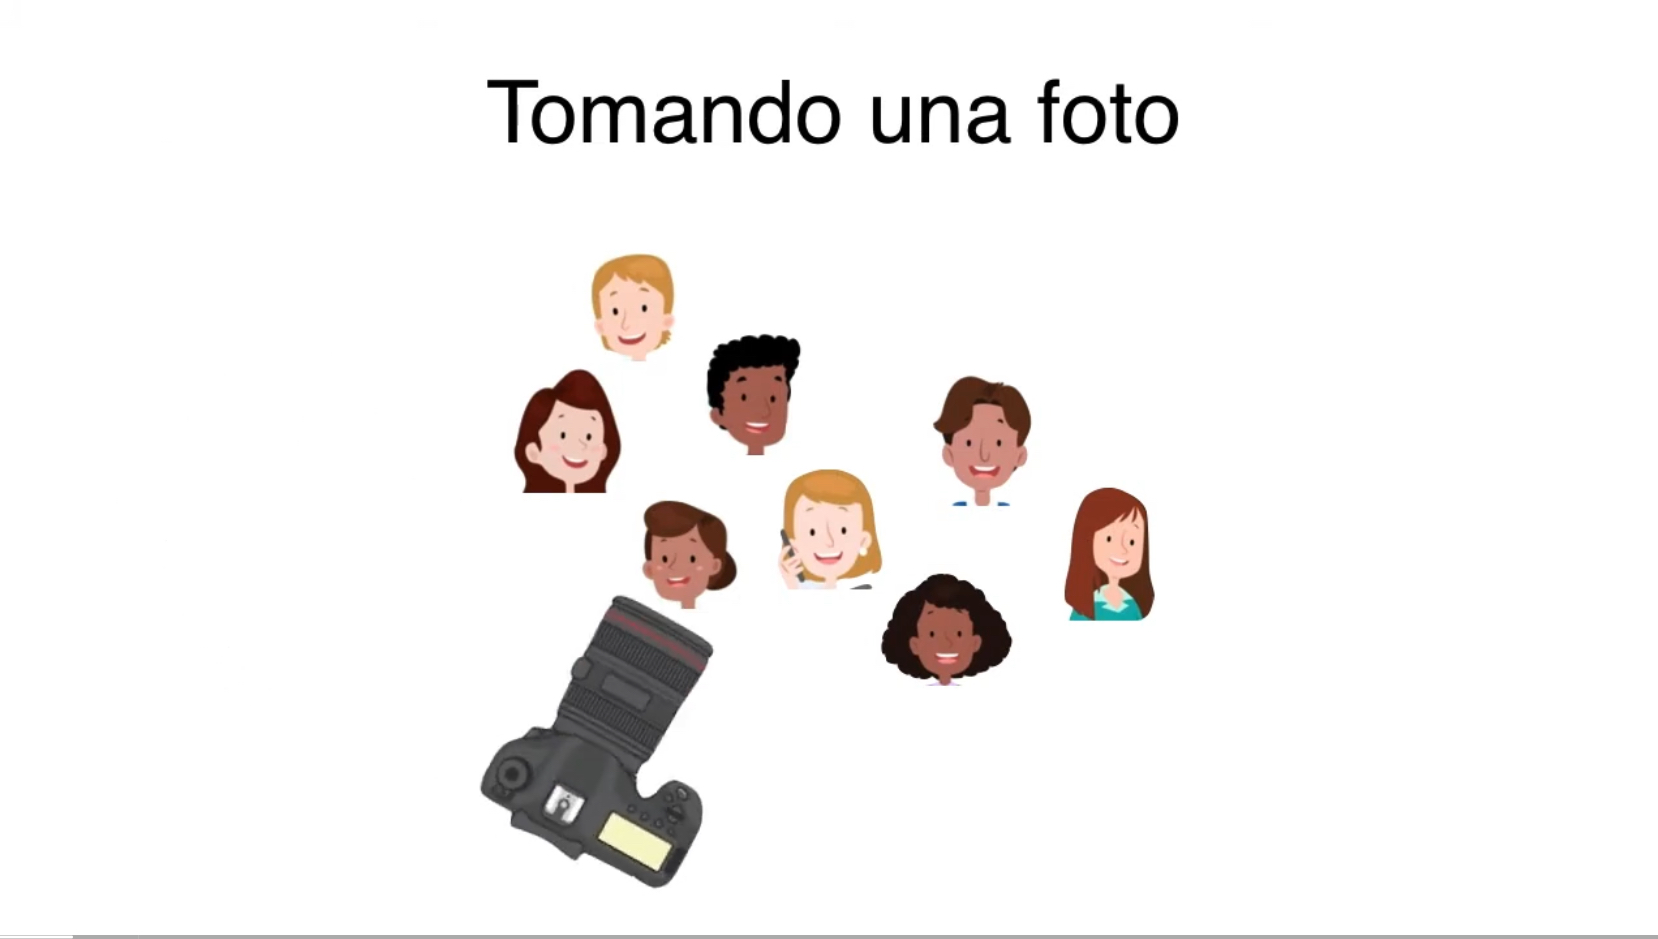
\includegraphics[width=0.9\textwidth]{PCA/IMG_3527.jpg}
		\caption{https://serrano.academy/espanol/}
	\end{figure}
\end{block}
\end{frame}

\begin{frame}
\frametitle{REDUCCIÓN DE DIMENSIONALIDAD}
\begin{block}{Análisis de Componentes Principales}	
	\begin{figure}
		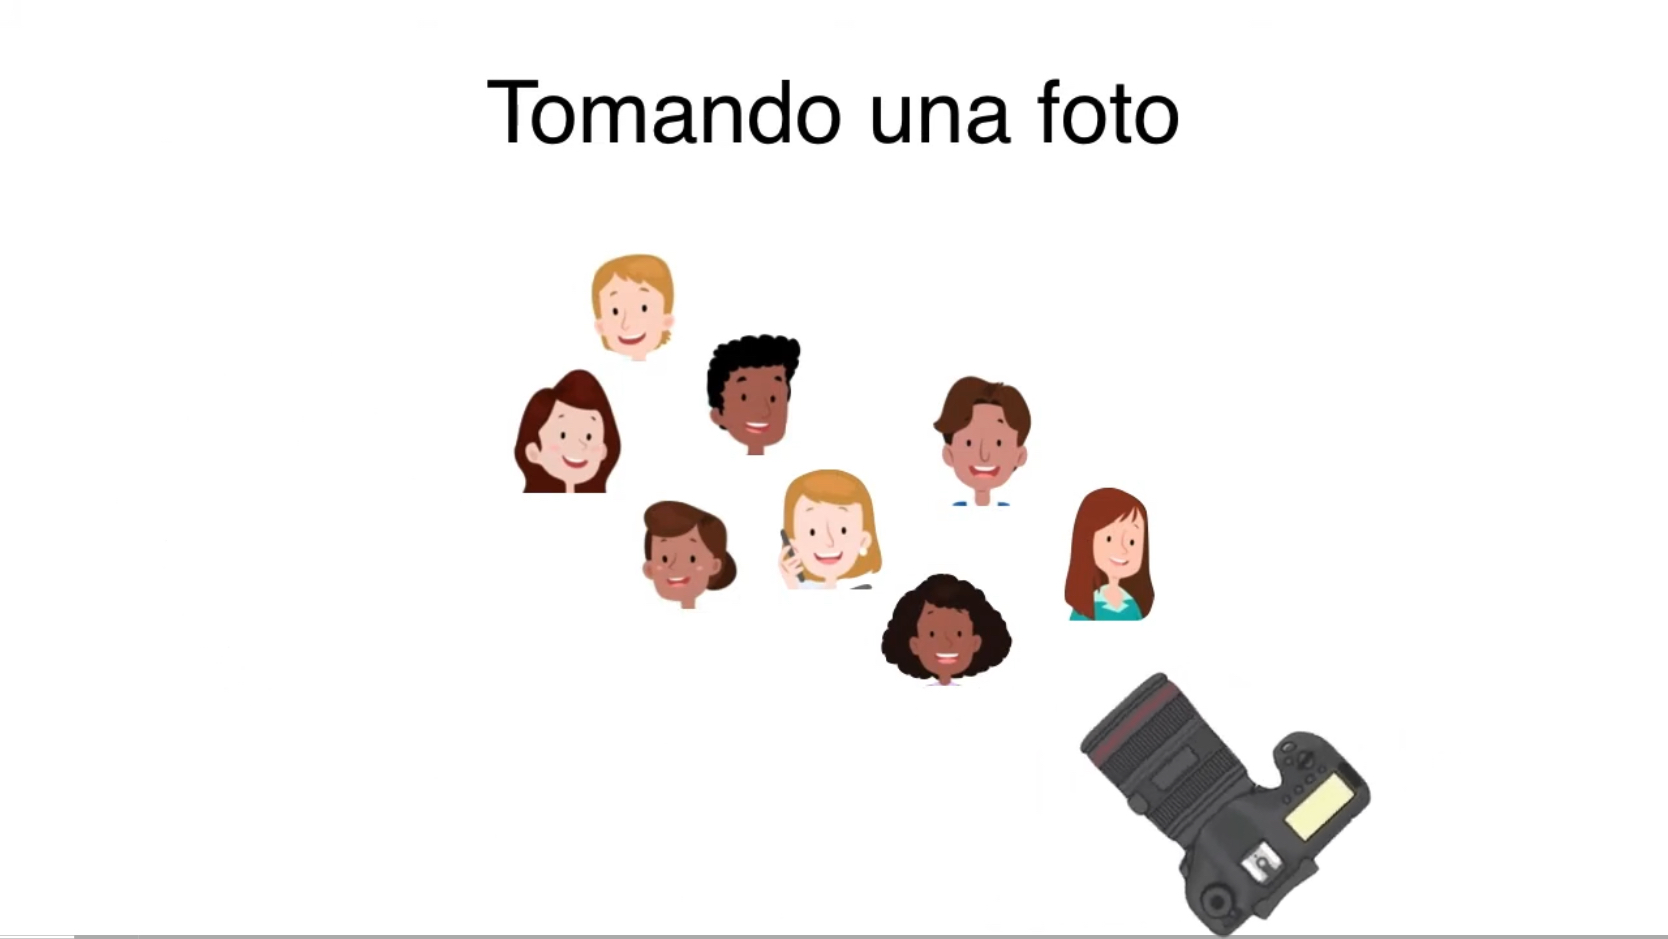
\includegraphics[width=0.9\textwidth]{PCA/IMG_3528.jpg}
		\caption{https://serrano.academy/espanol/}
	\end{figure}
\end{block}
\end{frame}

\begin{frame}
\frametitle{REDUCCIÓN DE DIMENSIONALIDAD}
\begin{block}{Análisis de Componentes Principales}	
	\begin{figure}
		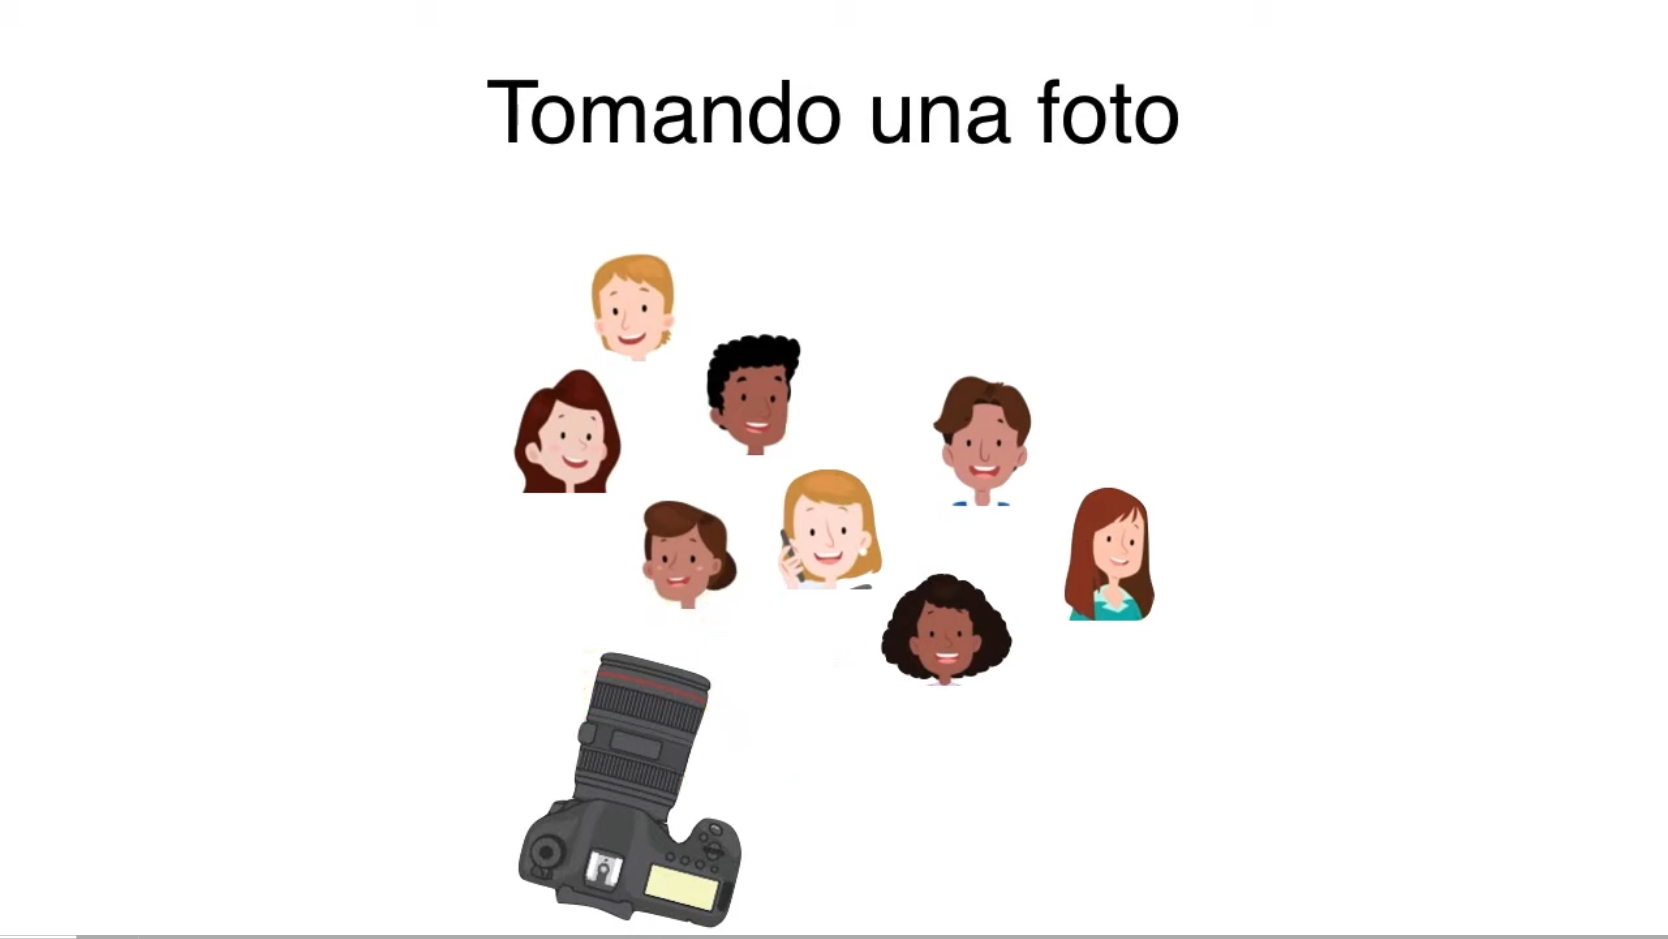
\includegraphics[width=0.9\textwidth]{PCA/IMG_3529.jpg}
		\caption{https://serrano.academy/espanol/}
	\end{figure}
\end{block}
\end{frame}

\begin{frame}
\frametitle{REDUCCIÓN DE DIMENSIONALIDAD}
\begin{block}{Análisis de Componentes Principales}	
	\begin{figure}
		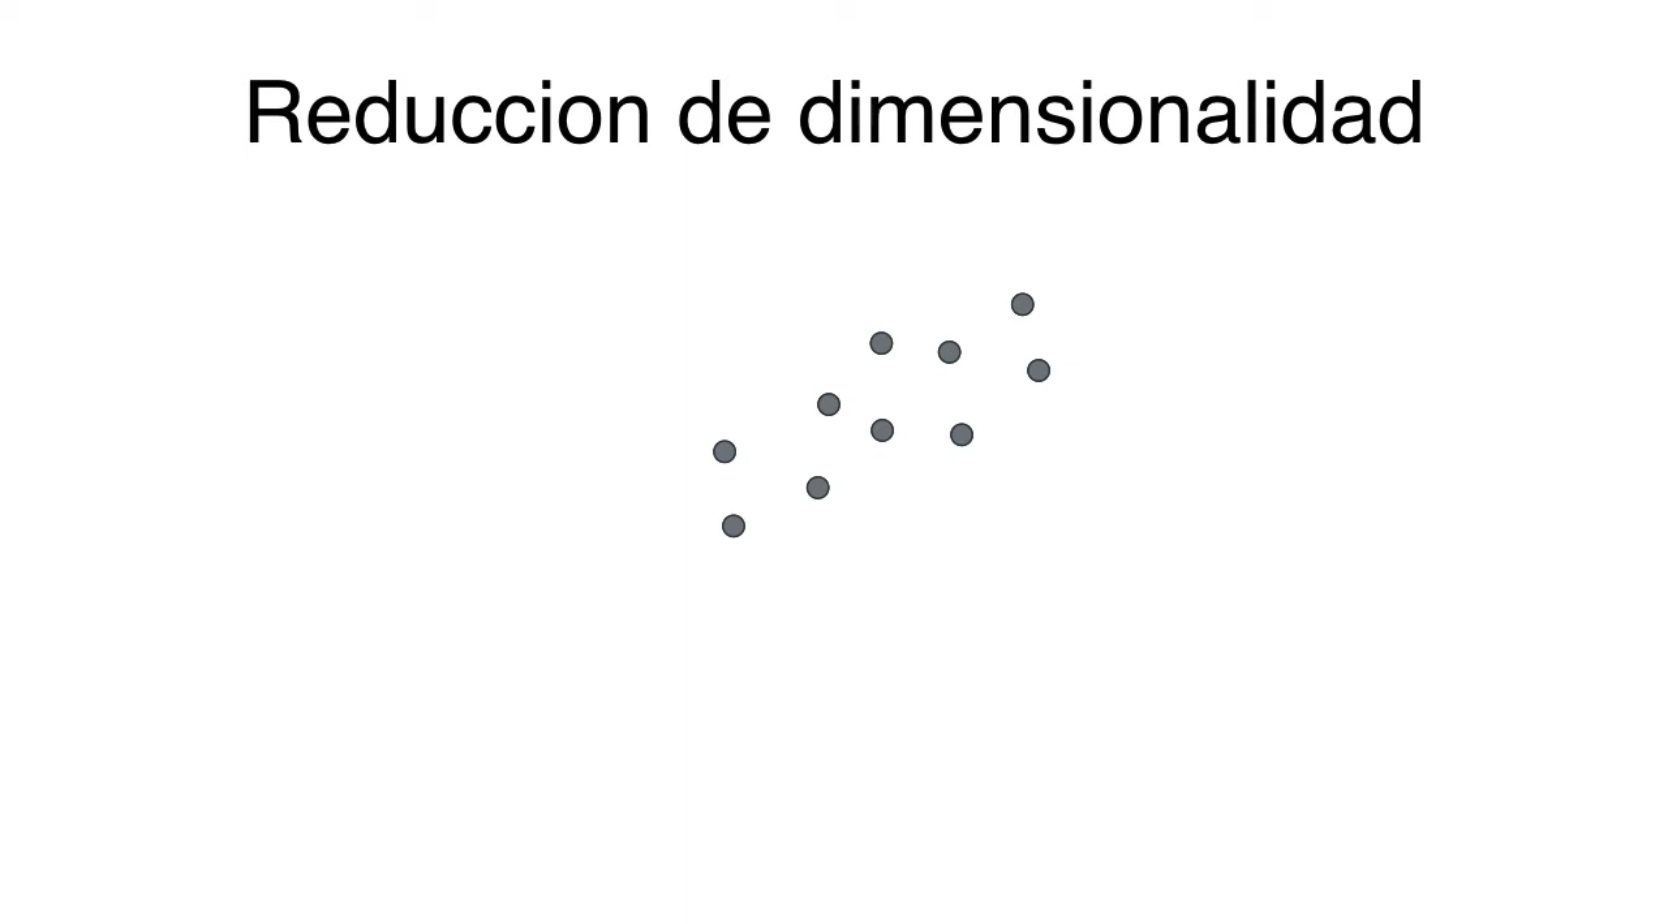
\includegraphics[width=0.9\textwidth]{PCA/IMG_3530.jpg}
		\caption{https://serrano.academy/espanol/}
	\end{figure}
\end{block}
\end{frame}

\begin{frame}
	\frametitle{REDUCCIÓN DE DIMENSIONALIDAD}
	\begin{block}{Análisis de Componentes Principales}	
		\begin{figure}
			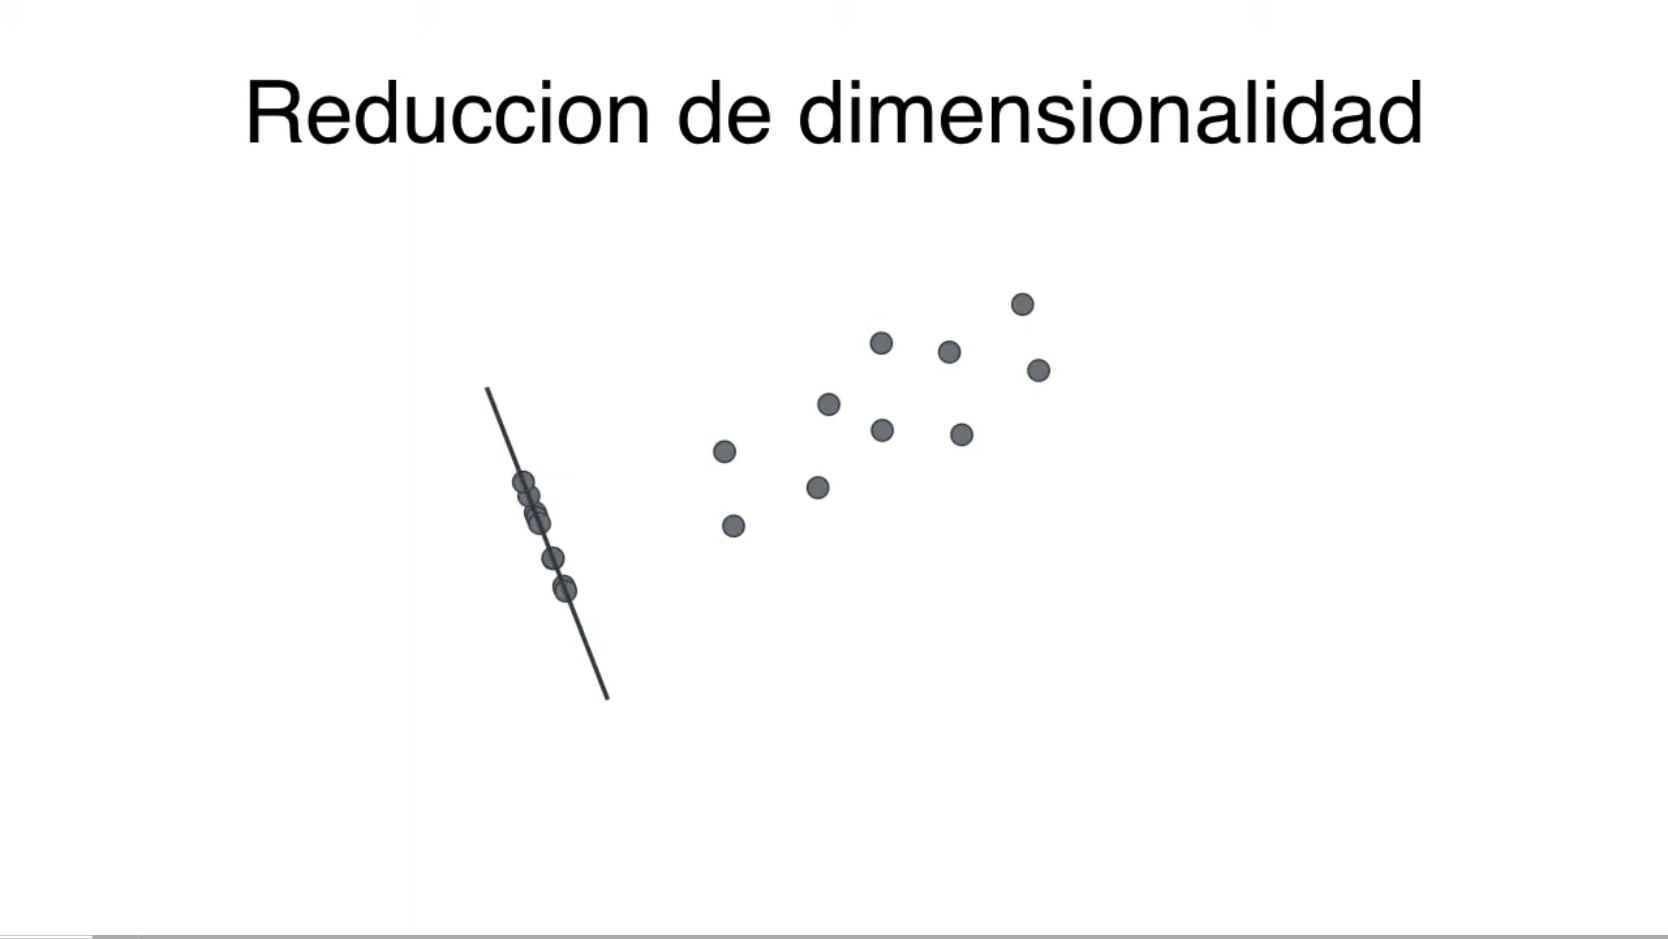
\includegraphics[width=0.9\textwidth]{PCA/IMG_3531.jpg}
			\caption{https://serrano.academy/espanol/}
		\end{figure}
	\end{block}
\end{frame}

\begin{frame}
	\frametitle{REDUCCIÓN DE DIMENSIONALIDAD}
	\begin{block}{Análisis de Componentes Principales}	
		\begin{figure}
			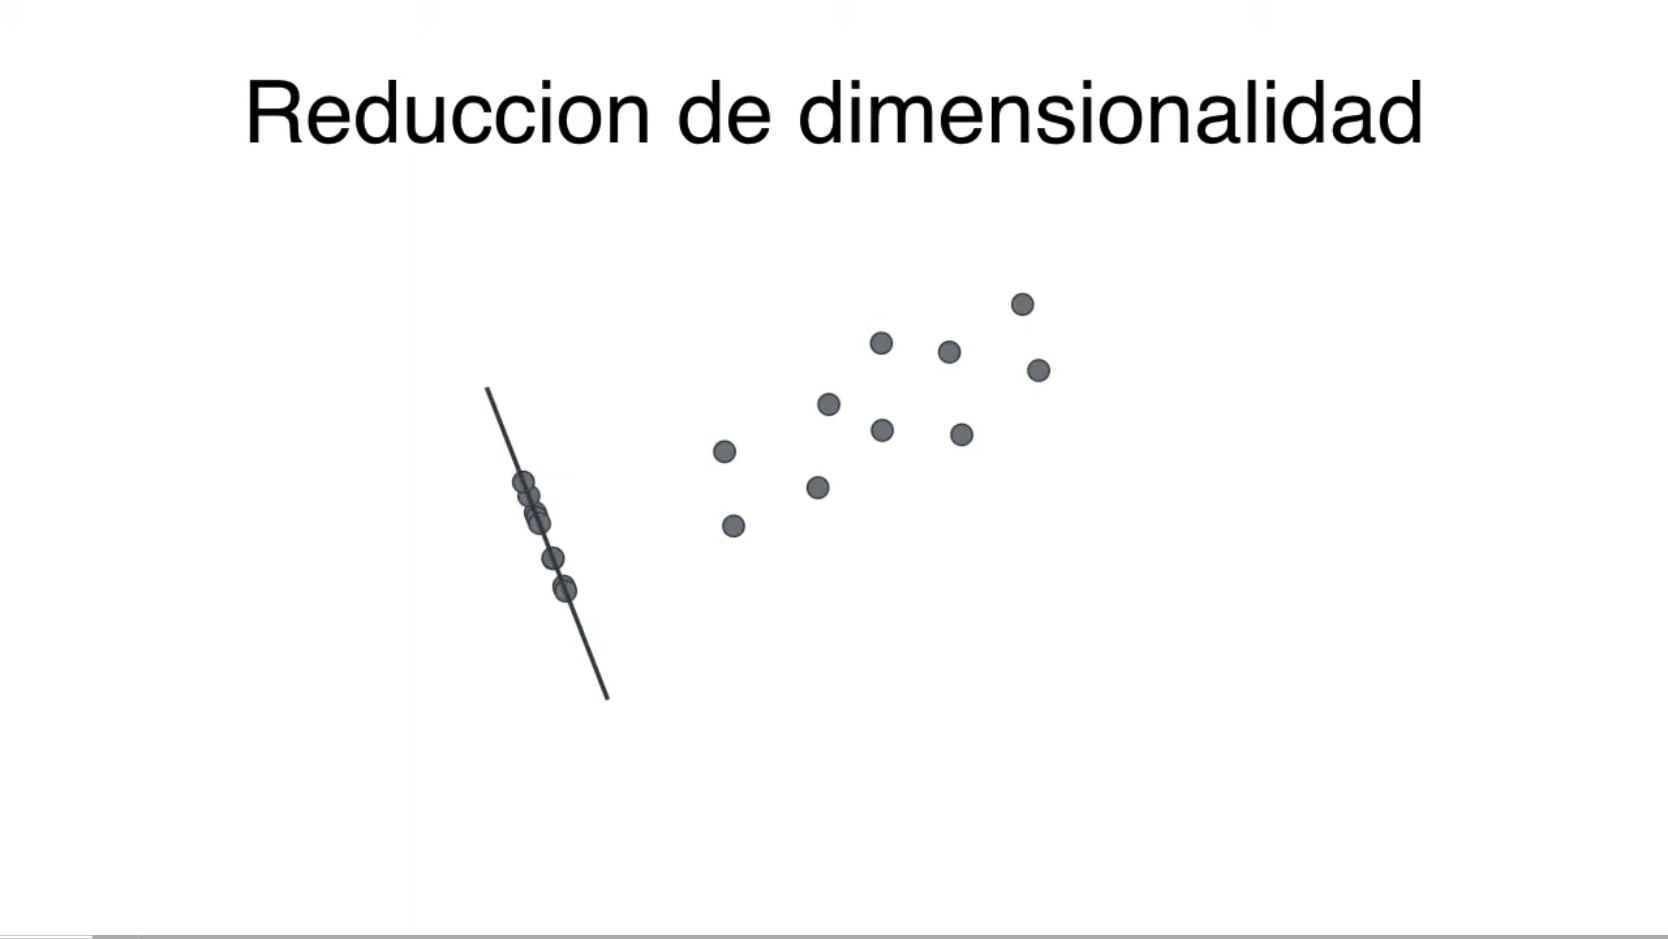
\includegraphics[width=0.9\textwidth]{PCA/IMG_3531.jpg}
			\caption{https://serrano.academy/espanol/}
		\end{figure}
	\end{block}
\end{frame}

\begin{frame}
	\frametitle{REDUCCIÓN DE DIMENSIONALIDAD}
	\begin{block}{Análisis de Componentes Principales}	
		\begin{figure}
			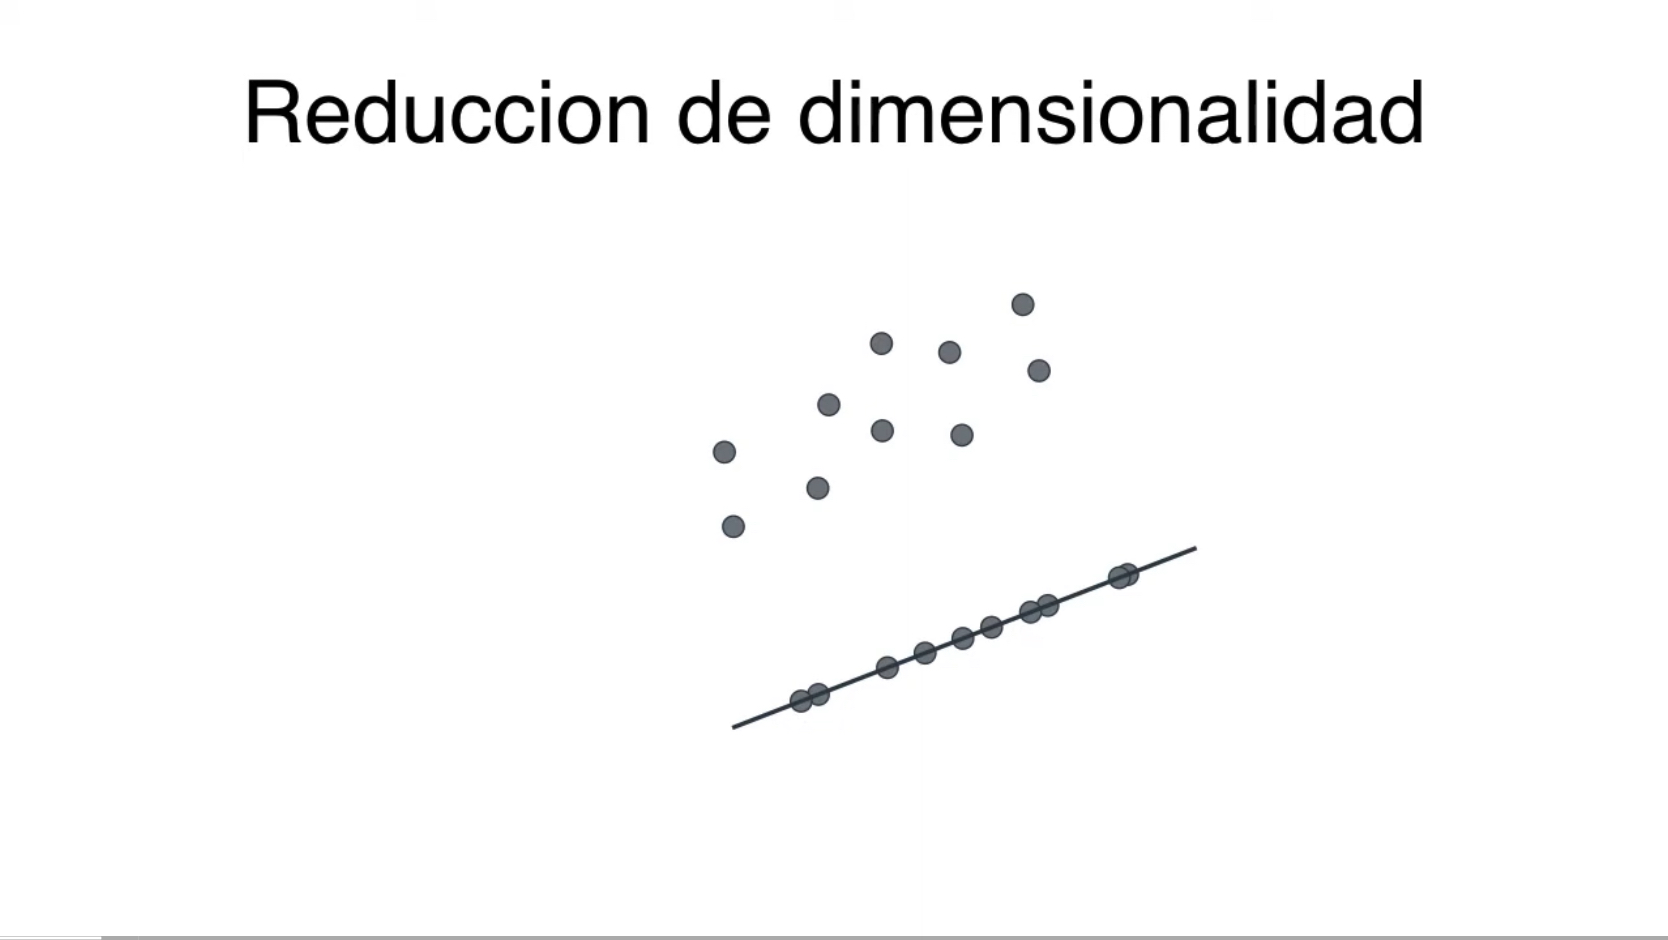
\includegraphics[width=0.9\textwidth]{PCA/IMG_3532.jpg}
			\caption{https://serrano.academy/espanol/}
		\end{figure}
	\end{block}
\end{frame}

\begin{frame}
	\frametitle{REDUCCIÓN DE DIMENSIONALIDAD}
	\begin{block}{Análisis de Componentes Principales}	
		\begin{figure}
			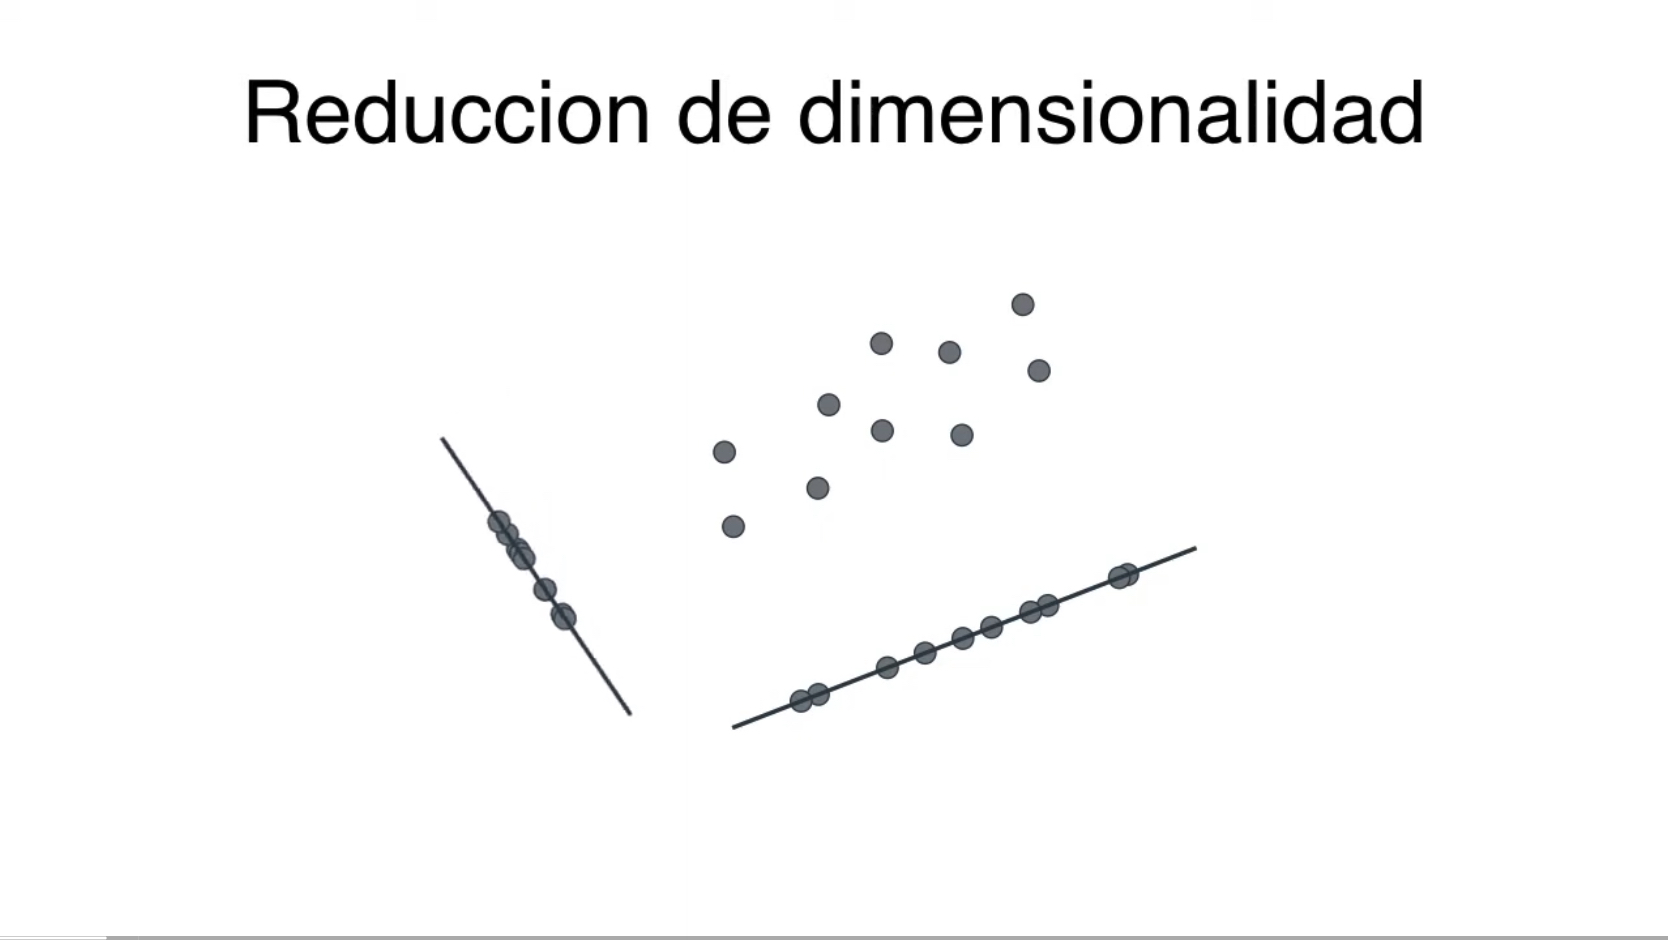
\includegraphics[width=0.9\textwidth]{PCA/IMG_3533.jpg}
			\caption{https://serrano.academy/espanol/}
		\end{figure}
	\end{block}
\end{frame}

\begin{frame}
	\frametitle{REDUCCIÓN DE DIMENSIONALIDAD}
	\begin{block}{Análisis de Componentes Principales}	
		\begin{figure}
			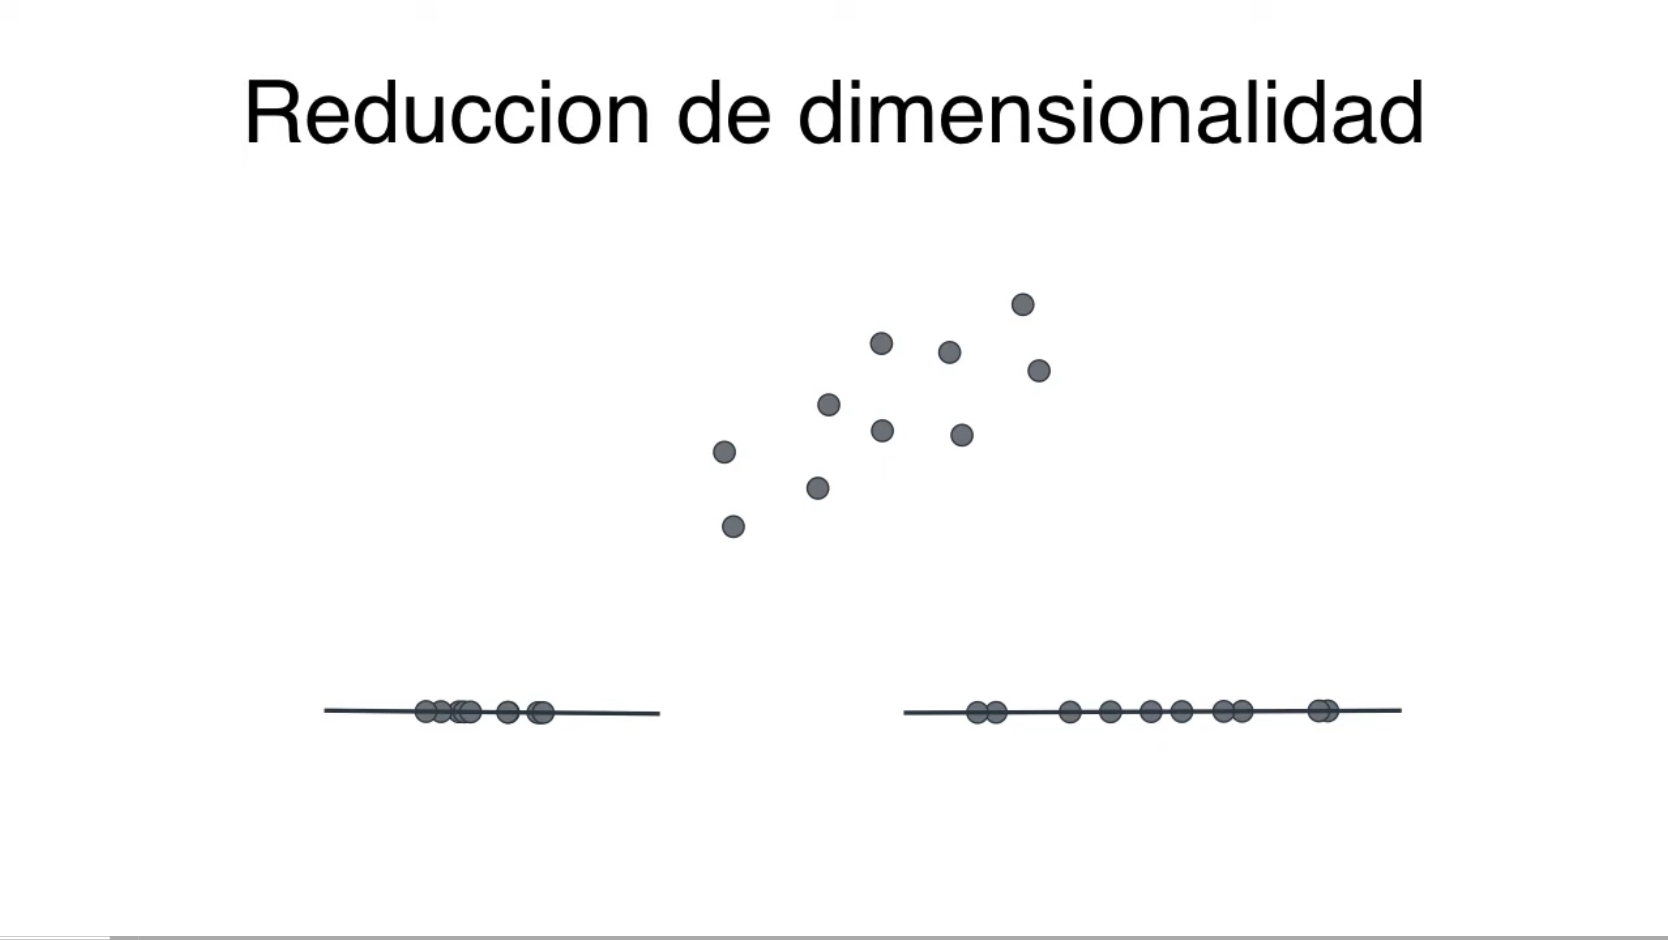
\includegraphics[width=0.9\textwidth]{PCA/IMG_3534.jpg}
			\caption{https://serrano.academy/espanol/}
		\end{figure}
	\end{block}
\end{frame}


\begin{frame}
	\frametitle{REDUCCIÓN DE DIMENSIONALIDAD}
	\begin{block}{Análisis de Componentes Principales}	
		\begin{figure}
			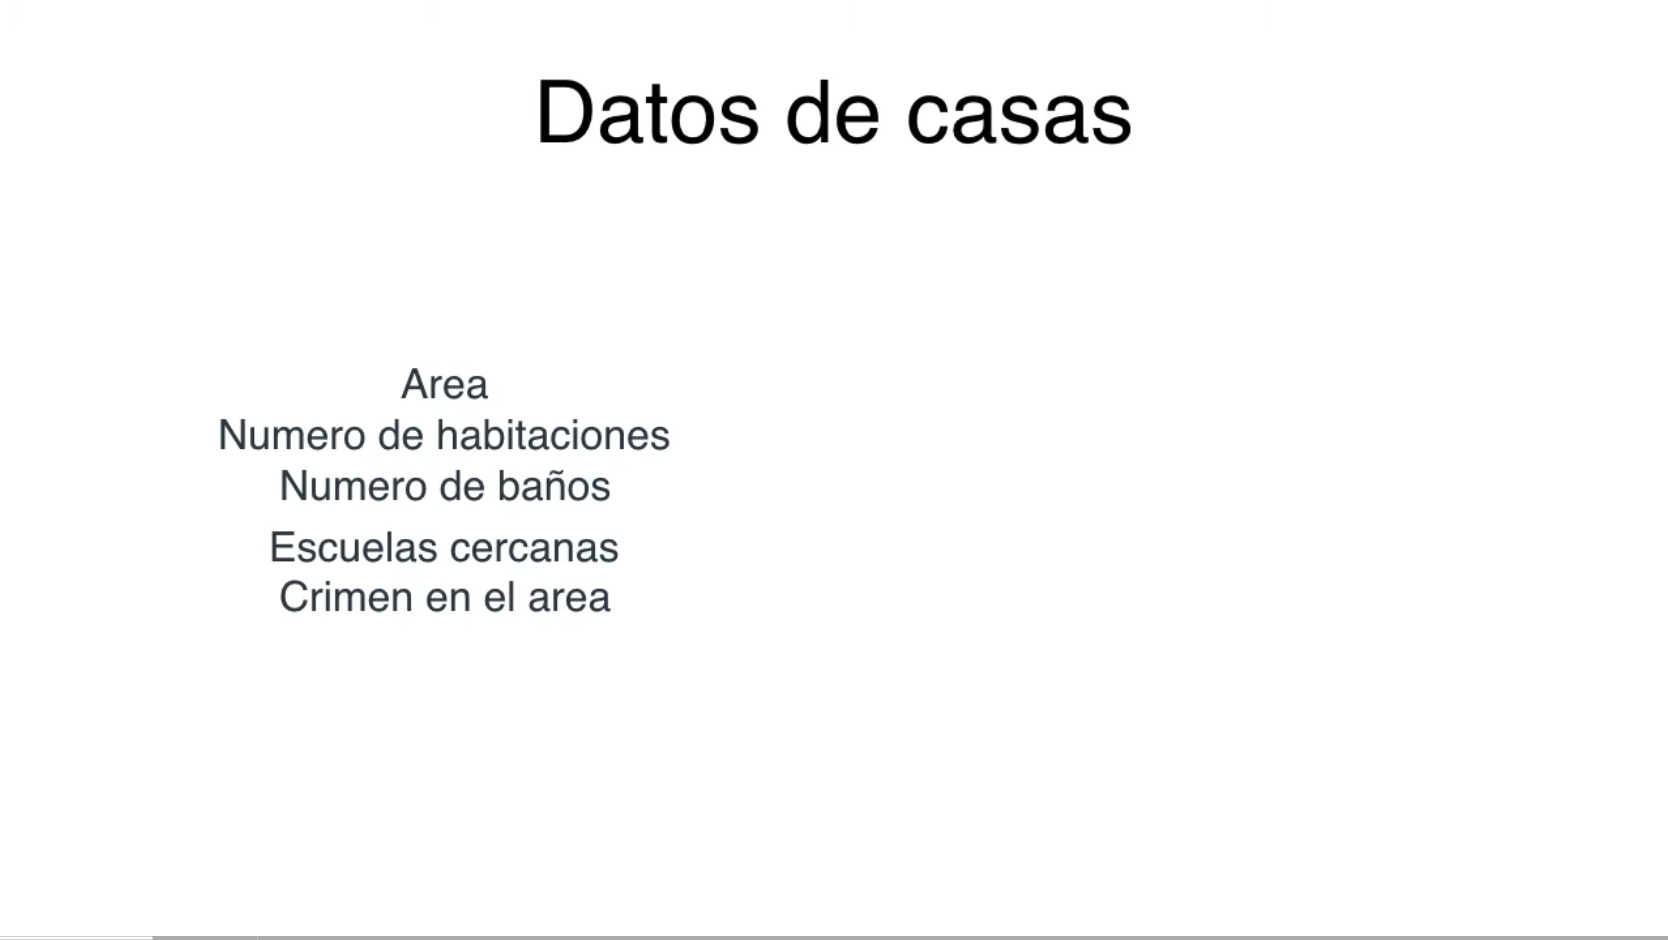
\includegraphics[width=0.9\textwidth]{PCA/IMG_3535.jpg}
			\caption{https://serrano.academy/espanol/}
		\end{figure}
	\end{block}
\end{frame}

\begin{frame}
	\frametitle{REDUCCIÓN DE DIMENSIONALIDAD}
	\begin{block}{Análisis de Componentes Principales}	
		\begin{figure}
			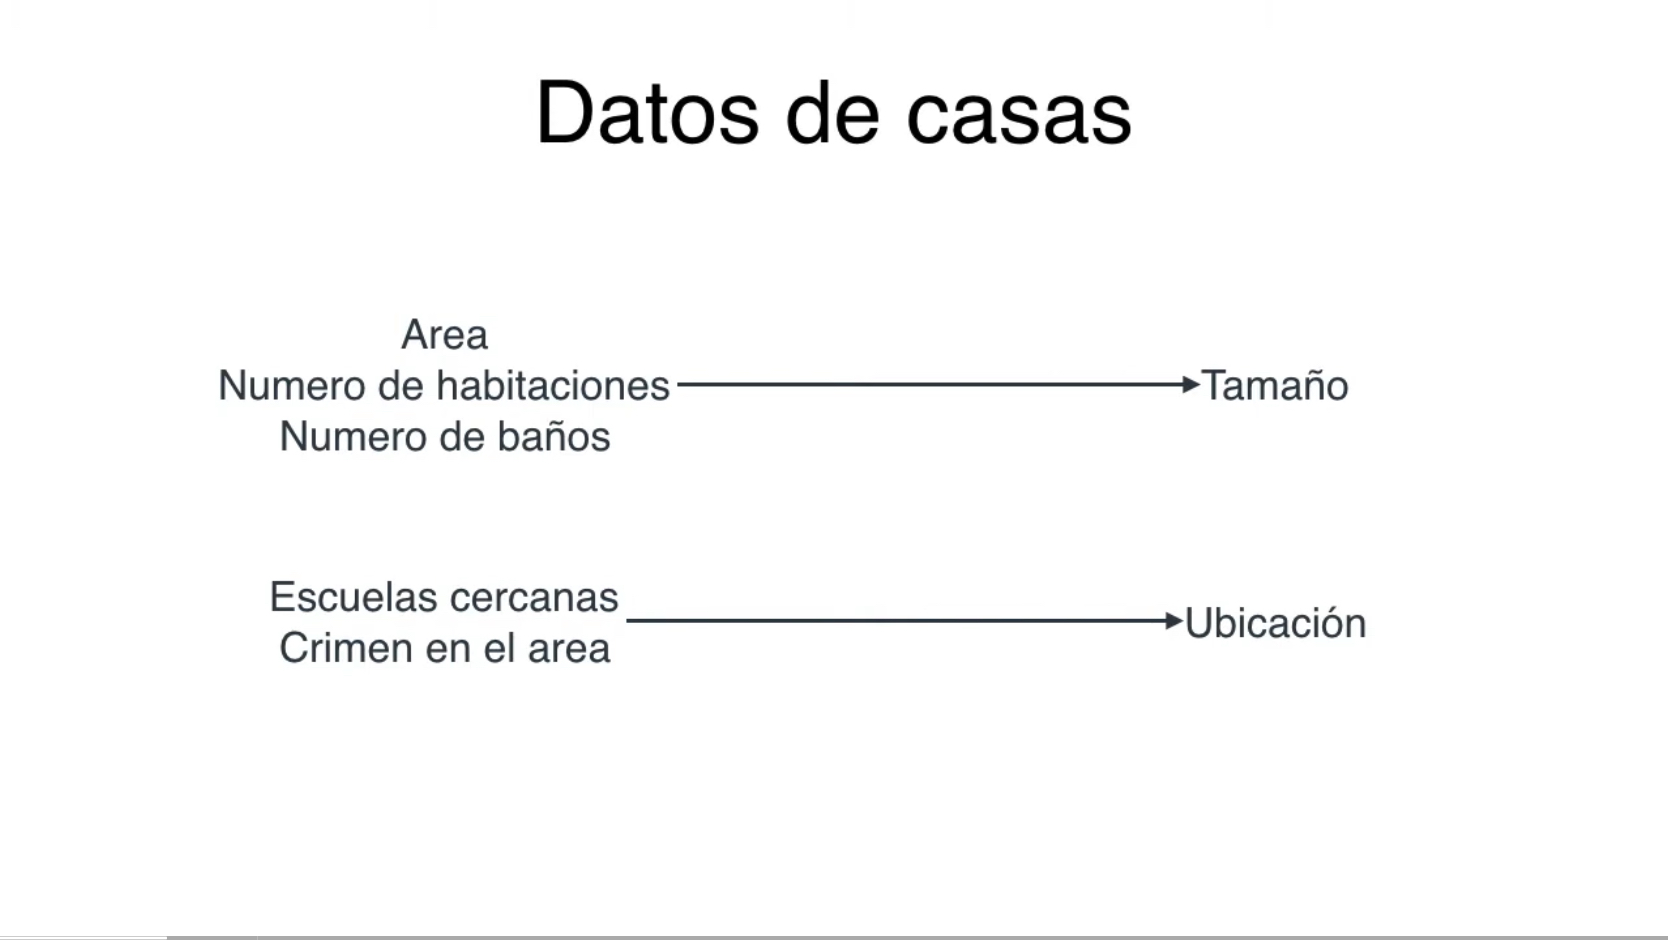
\includegraphics[width=0.9\textwidth]{PCA/IMG_3536.jpg}
			\caption{https://serrano.academy/espanol/}
		\end{figure}
	\end{block}
\end{frame}

\begin{frame}
	\frametitle{REDUCCIÓN DE DIMENSIONALIDAD}
	\begin{block}{Análisis de Componentes Principales}	
		\begin{figure}
			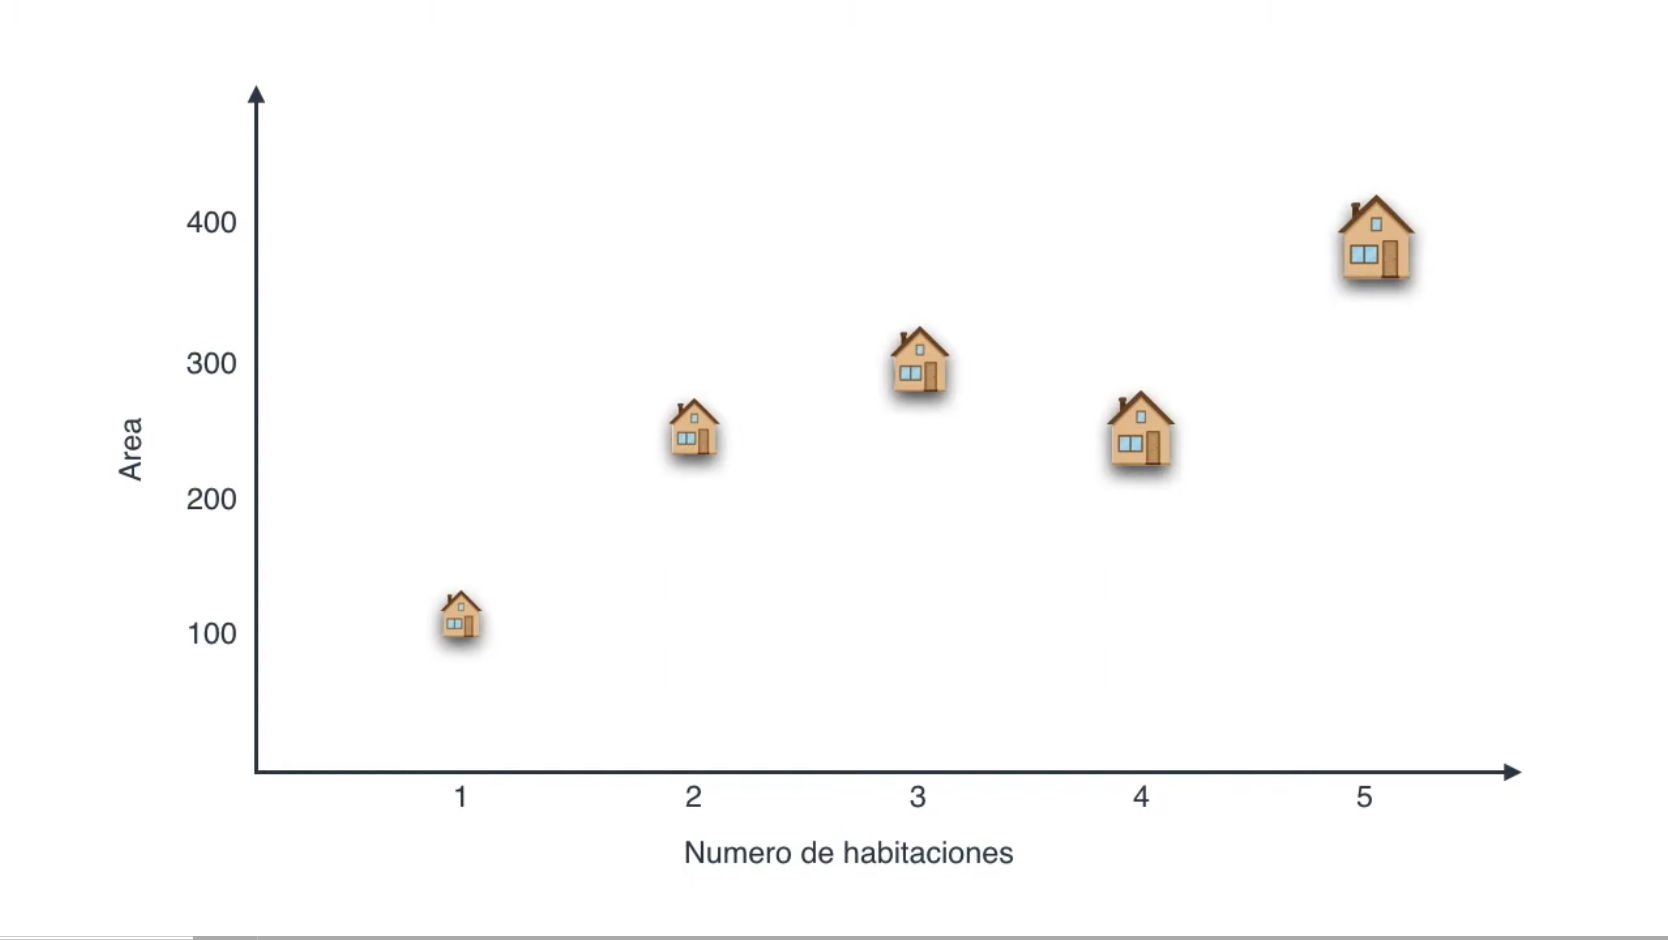
\includegraphics[width=0.9\textwidth]{PCA/IMG_3537.jpg}
			\caption{https://serrano.academy/espanol/}
		\end{figure}
	\end{block}
\end{frame}

\begin{frame}
	\frametitle{REDUCCIÓN DE DIMENSIONALIDAD}
	\begin{block}{Análisis de Componentes Principales}	
		\begin{figure}
			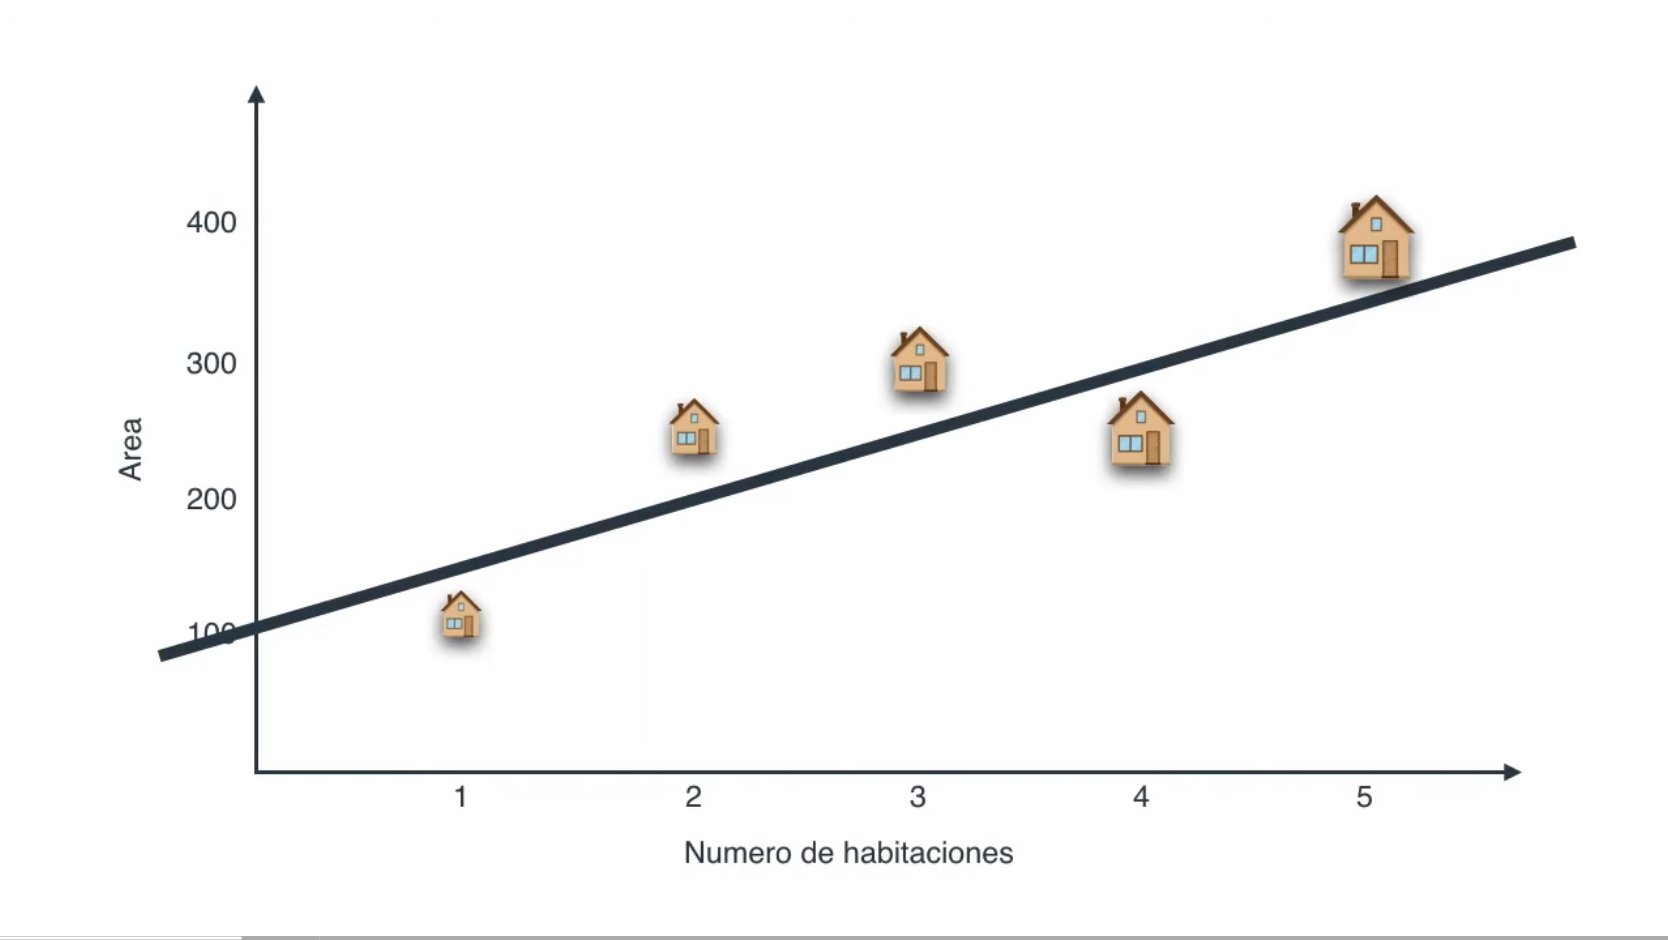
\includegraphics[width=0.9\textwidth]{PCA/IMG_3538.jpg}
			\caption{https://serrano.academy/espanol/}
		\end{figure}
	\end{block}
\end{frame}

\begin{frame}
	\frametitle{REDUCCIÓN DE DIMENSIONALIDAD}
	\begin{block}{Análisis de Componentes Principales}	
		\begin{figure}
			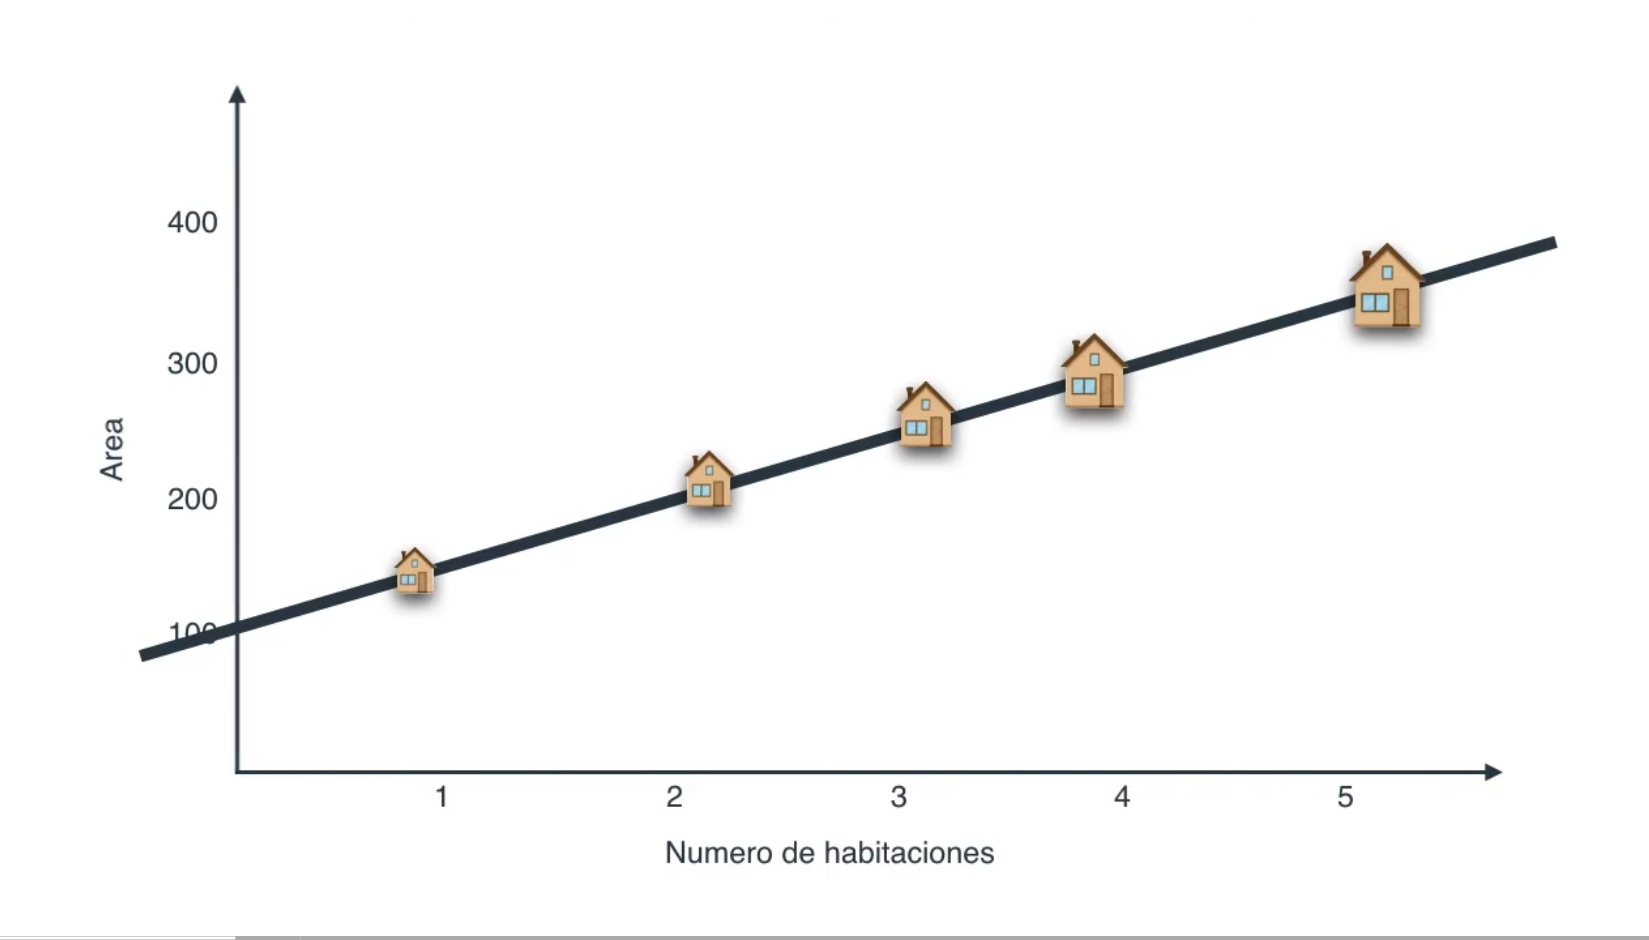
\includegraphics[width=0.9\textwidth]{PCA/IMG_3539.jpg}
			\caption{https://serrano.academy/espanol/}
		\end{figure}
	\end{block}
\end{frame}

\begin{frame}
	\frametitle{REDUCCIÓN DE DIMENSIONALIDAD}
	\begin{block}{Análisis de Componentes Principales}	
		\begin{figure}
			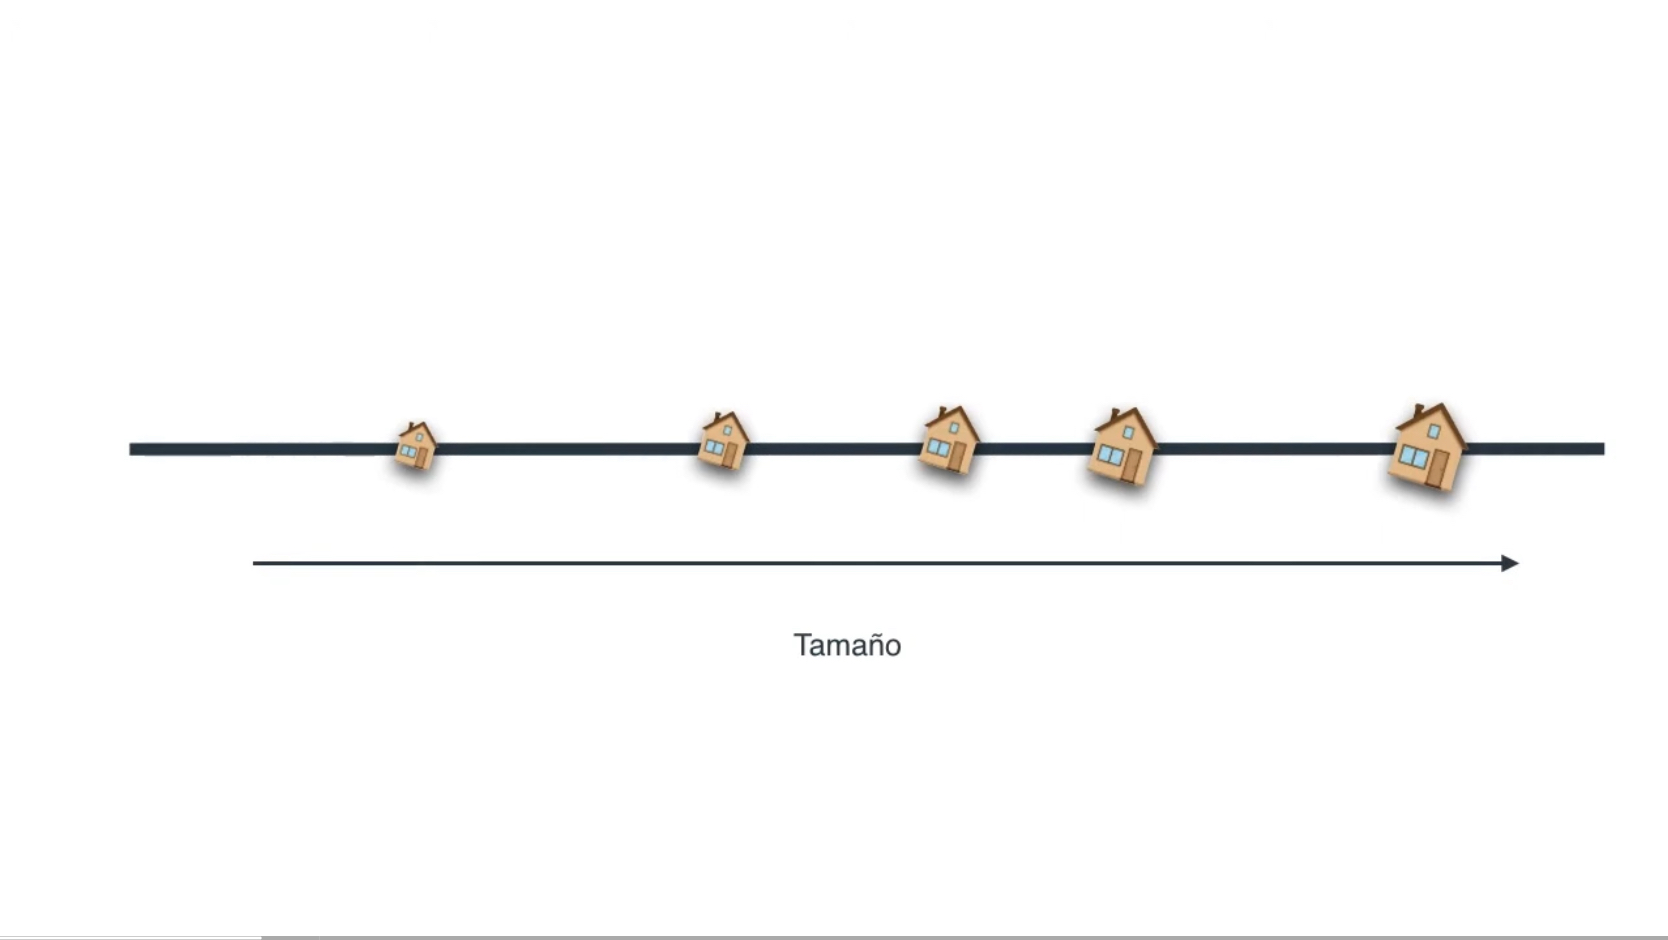
\includegraphics[width=0.9\textwidth]{PCA/IMG_3540.jpg}
			\caption{https://serrano.academy/espanol/}
		\end{figure}
	\end{block}
\end{frame}


\begin{frame}
	\frametitle{REDUCCIÓN DE DIMENSIONALIDAD}
	\begin{block}{Análisis de Componentes Principales}	
		\begin{figure}
			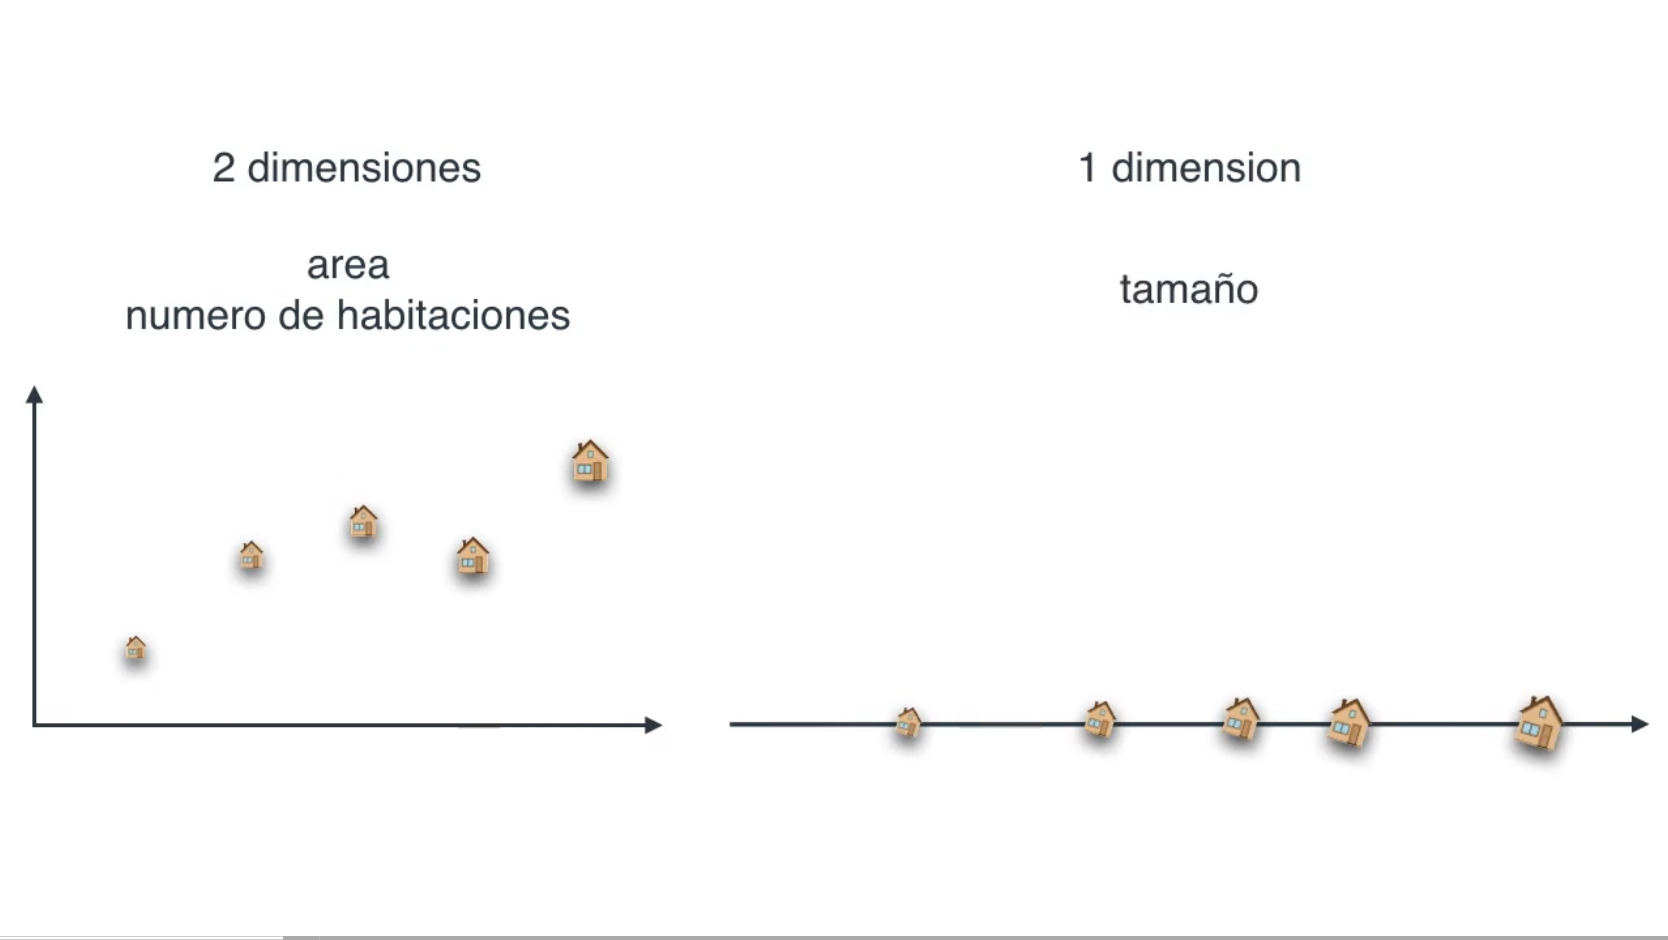
\includegraphics[width=0.9\textwidth]{PCA/IMG_3541.jpg}
			\caption{https://serrano.academy/espanol/}
		\end{figure}
	\end{block}
\end{frame}


\begin{frame}
	\frametitle{REDUCCIÓN DE DIMENSIONALIDAD}
	\begin{block}{Análisis de Componentes Principales}	
		\begin{figure}
			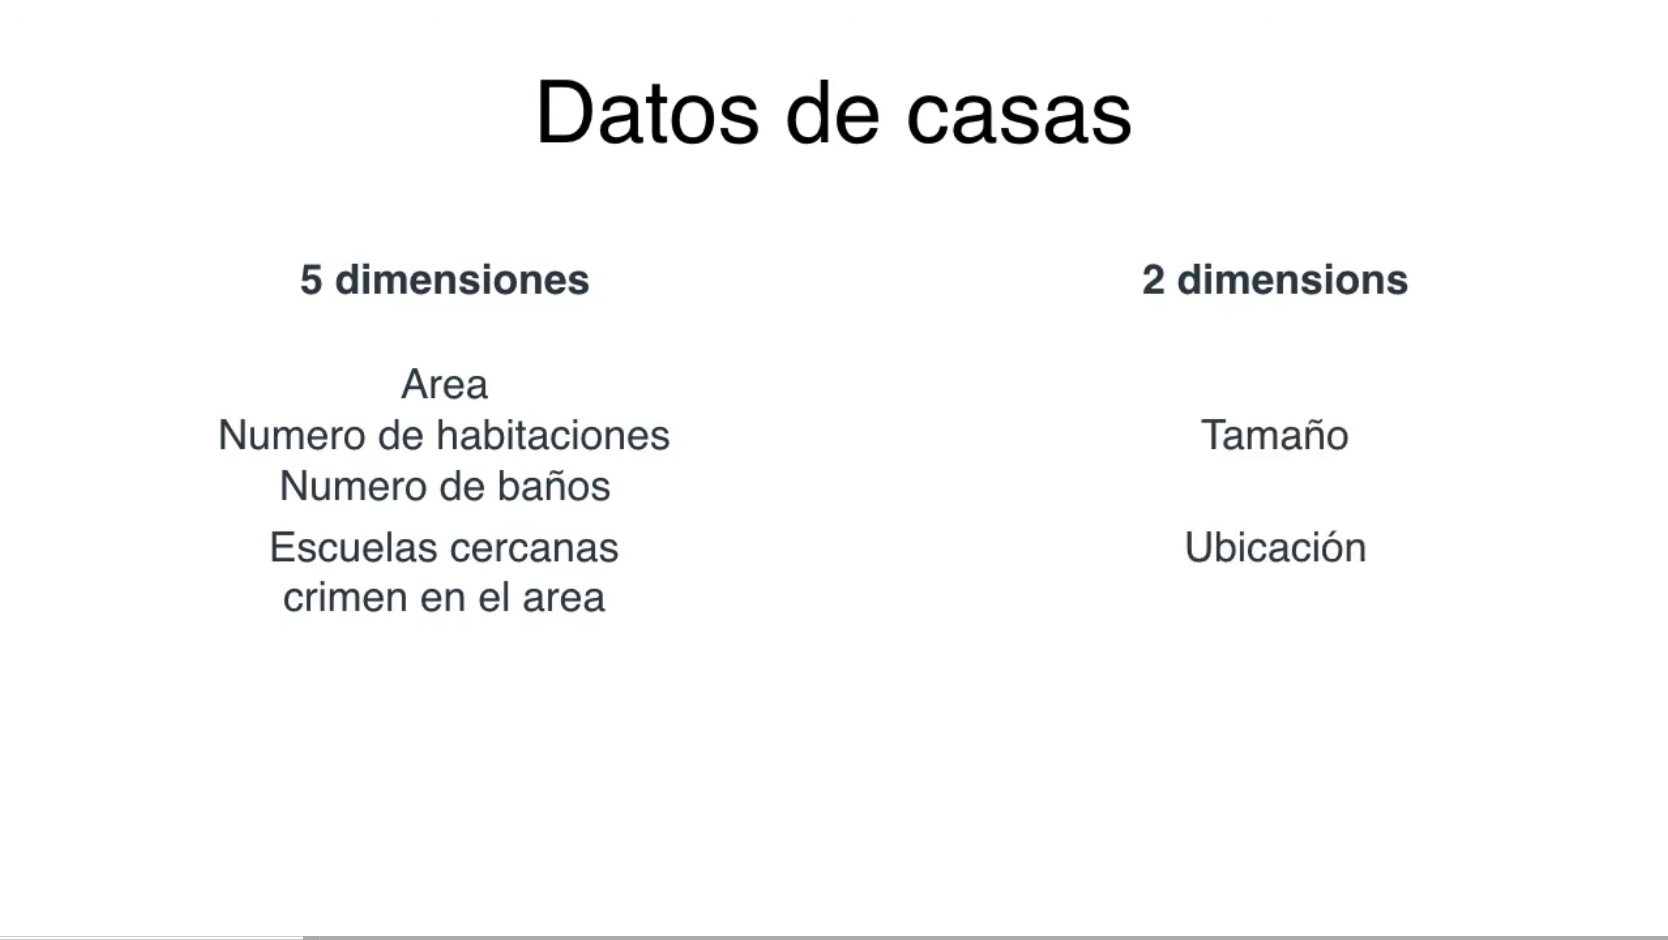
\includegraphics[width=0.9\textwidth]{PCA/IMG_3542.jpg}
			\caption{https://serrano.academy/espanol/}
		\end{figure}
	\end{block}
\end{frame}


\begin{frame}
	\frametitle{REDUCCIÓN DE DIMENSIONALIDAD}
	\begin{block}{Análisis de Componentes Principales}	
		\textbf{Promedio, varianza, covarianza}
	\end{block}
\end{frame}

\begin{frame}
	\frametitle{REDUCCIÓN DE DIMENSIONALIDAD}
	\begin{block}{Análisis de Componentes Principales}	
		\begin{figure}
			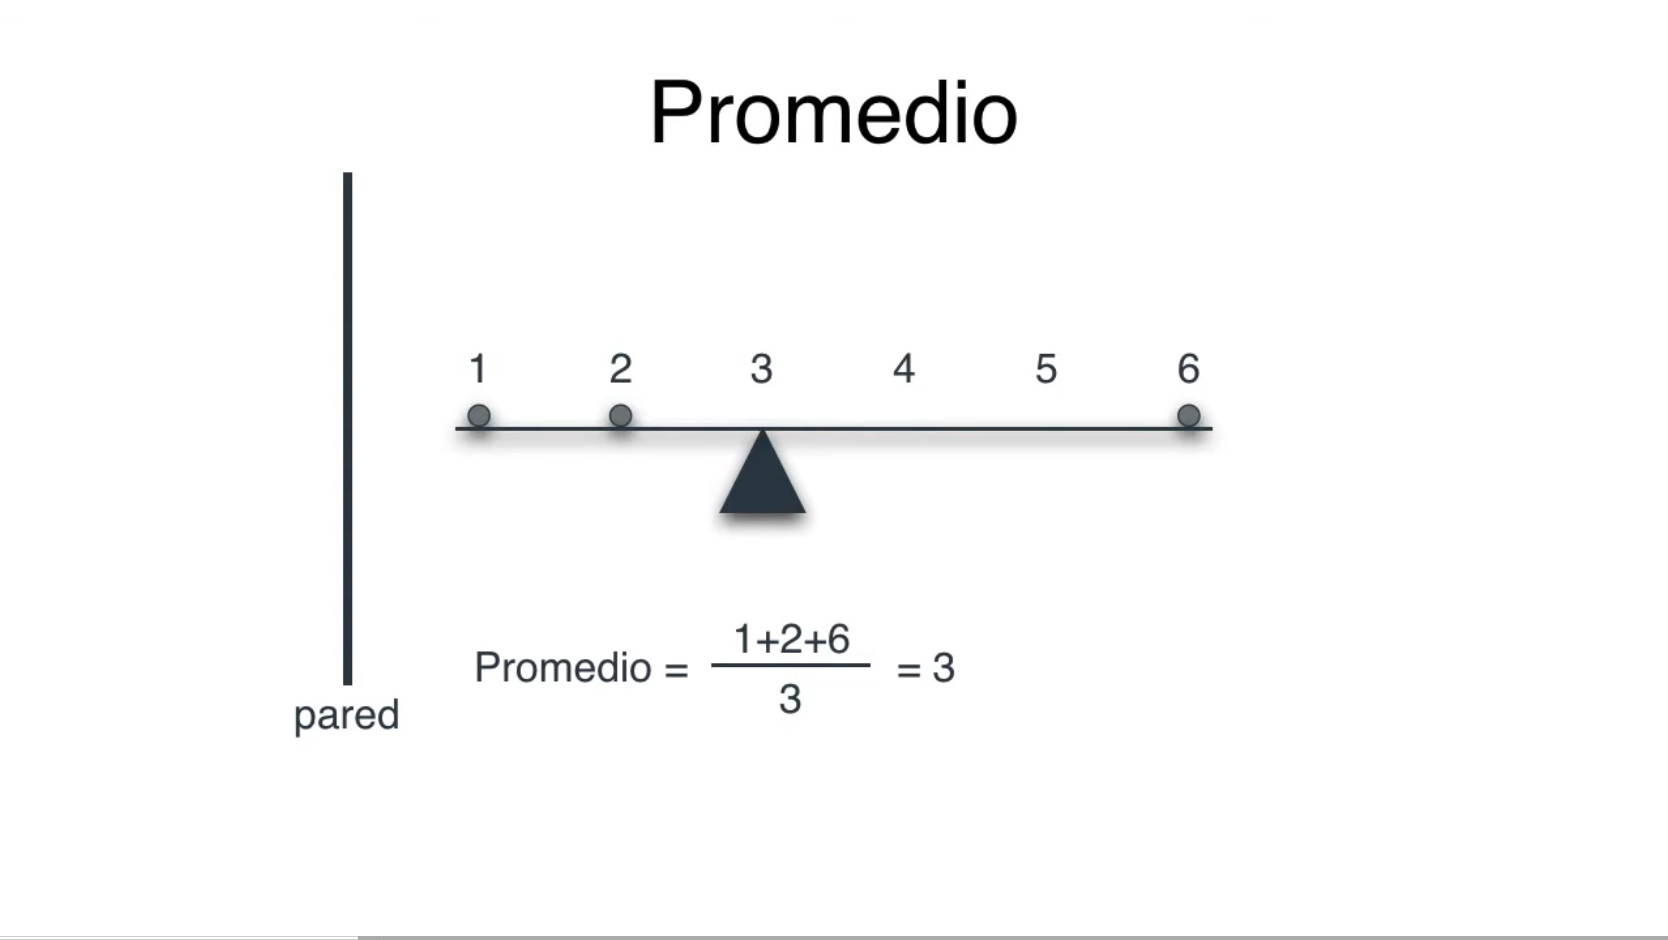
\includegraphics[width=0.9\textwidth]{PCA/IMG_3544.jpg}
			\caption{https://serrano.academy/espanol/}
		\end{figure}
	\end{block}
\end{frame}


\begin{frame}
	\frametitle{REDUCCIÓN DE DIMENSIONALIDAD}
	\begin{block}{Análisis de Componentes Principales}	
		\begin{figure}
			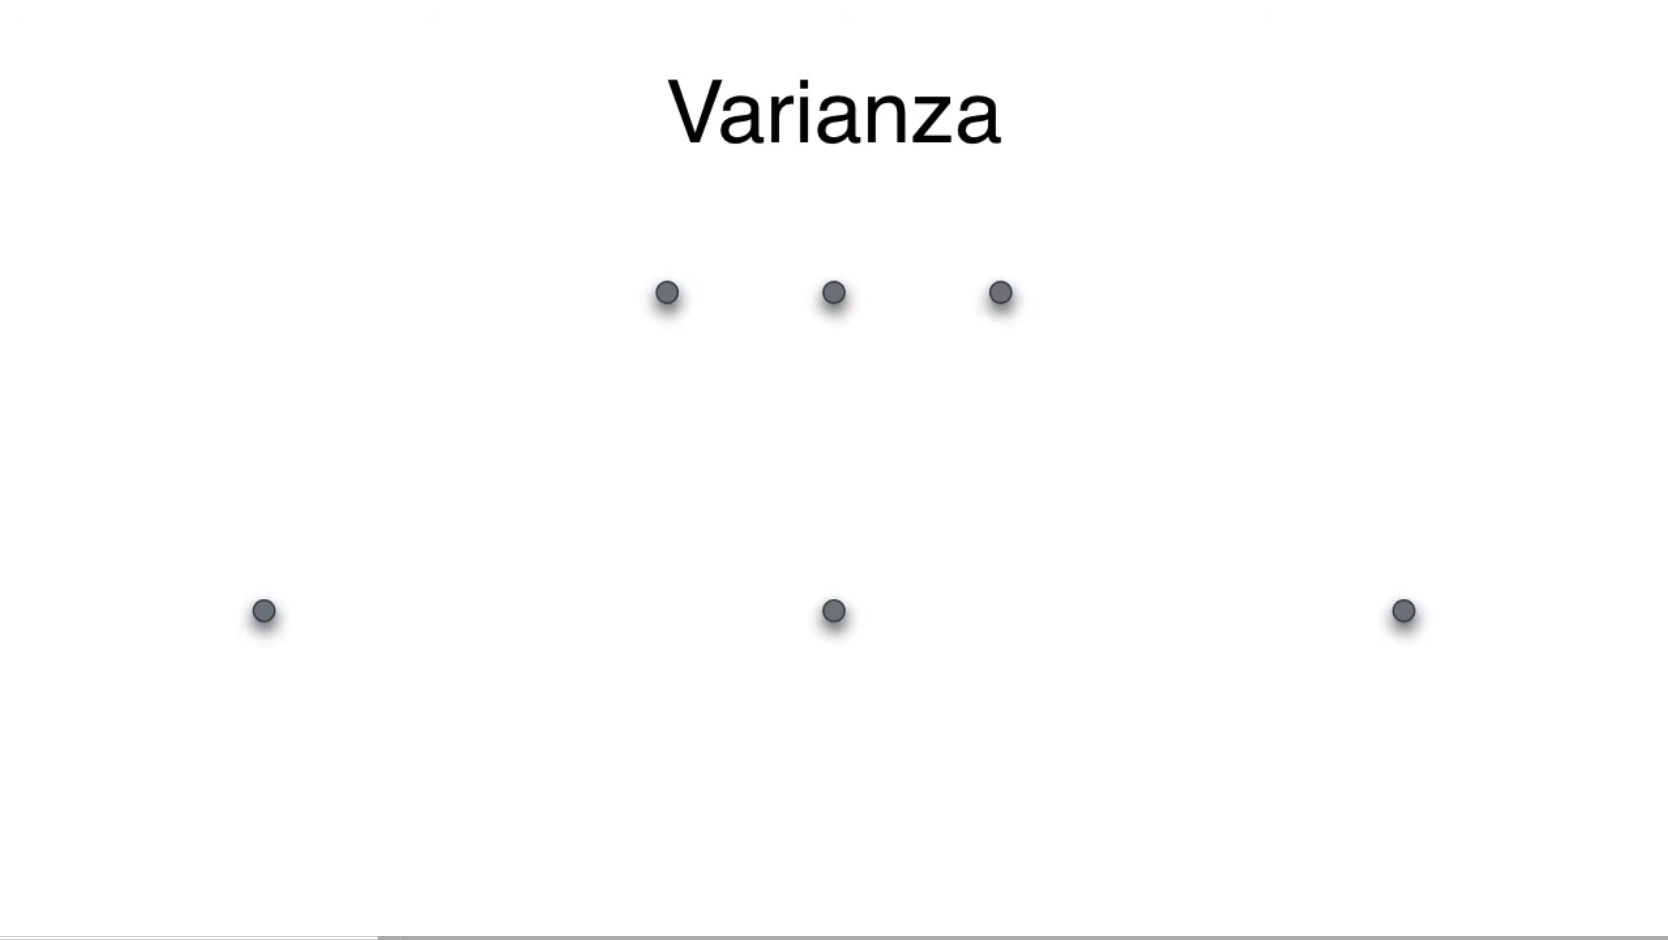
\includegraphics[width=0.9\textwidth]{PCA/IMG_3545.jpg}
			\caption{https://serrano.academy/espanol/}
		\end{figure}
	\end{block}
\end{frame}

\begin{frame}
	\frametitle{REDUCCIÓN DE DIMENSIONALIDAD}
	\begin{block}{Análisis de Componentes Principales}	
		\begin{figure}
			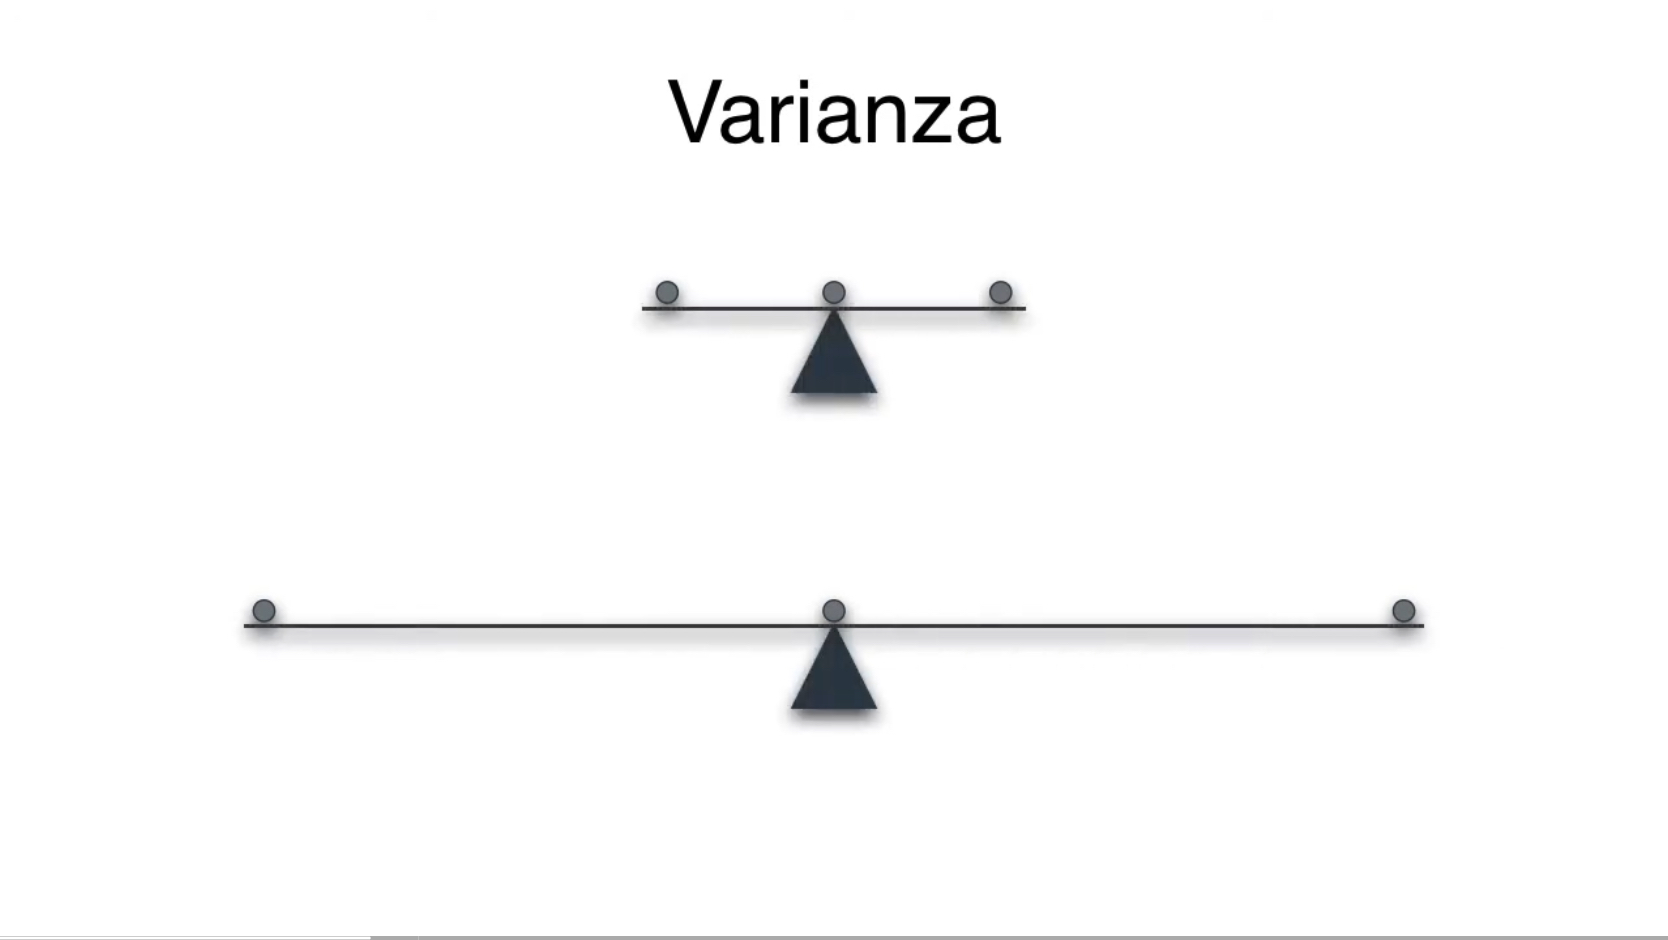
\includegraphics[width=0.9\textwidth]{PCA/IMG_3546.jpg}
			\caption{https://serrano.academy/espanol/}
		\end{figure}
	\end{block}
\end{frame}


\begin{frame}
	\frametitle{REDUCCIÓN DE DIMENSIONALIDAD}
	\begin{block}{Análisis de Componentes Principales}	
		\begin{figure}
			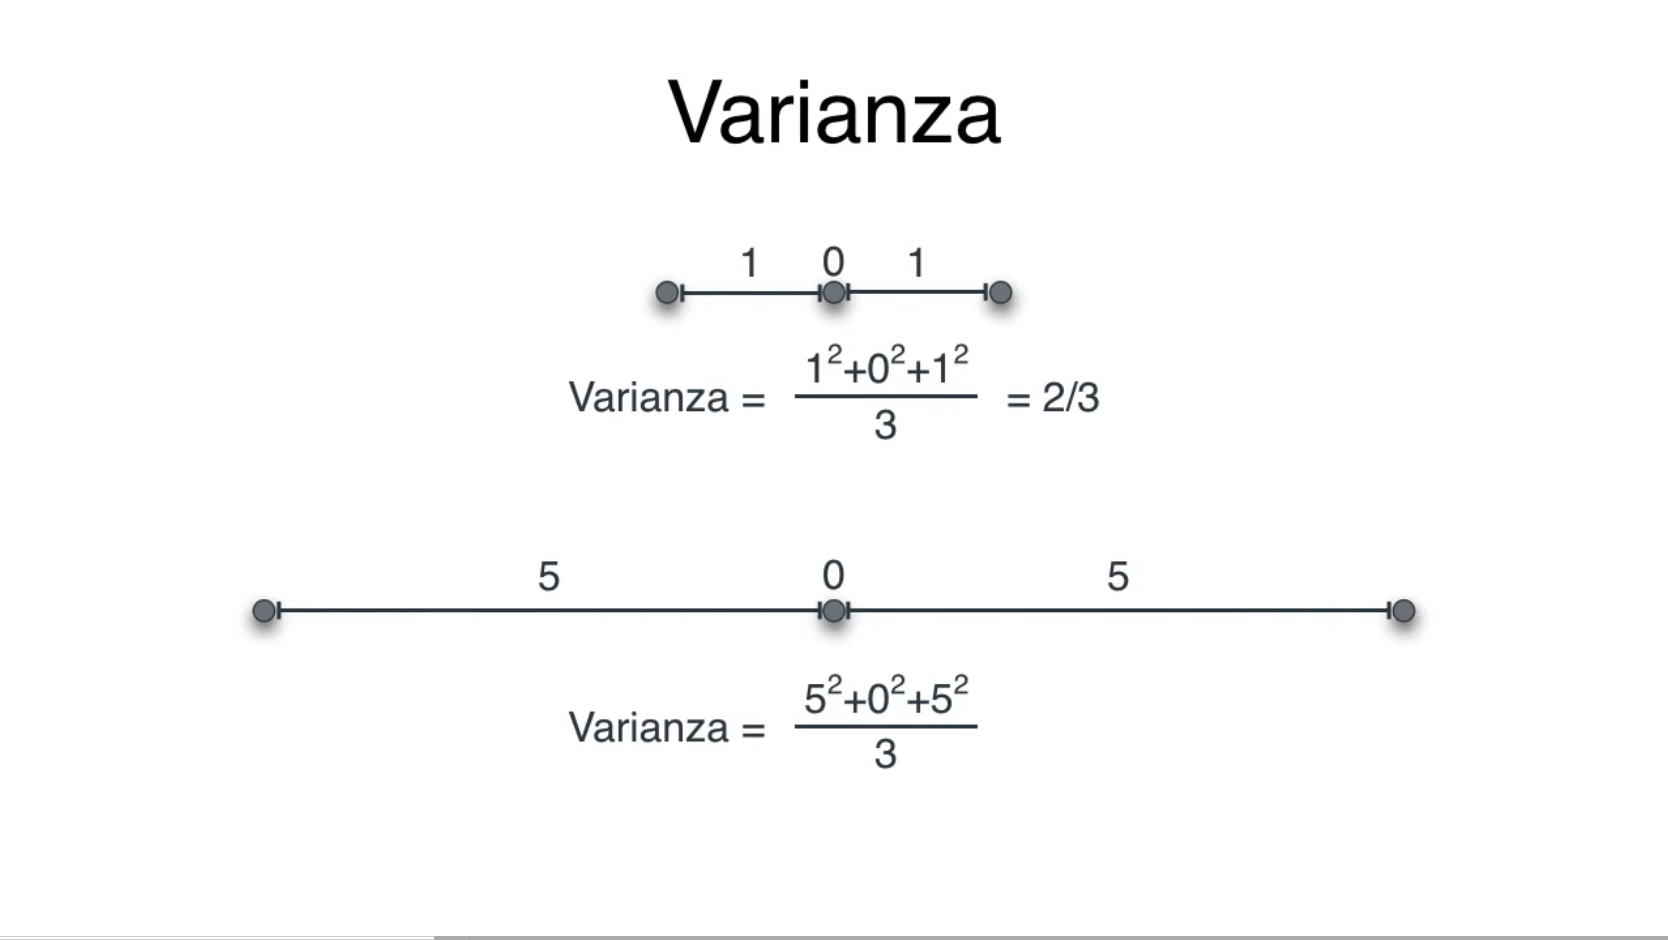
\includegraphics[width=0.9\textwidth]{PCA/IMG_3547.jpg}
			\caption{https://serrano.academy/espanol/}
		\end{figure}
	\end{block}
\end{frame}


\begin{frame}
	\frametitle{REDUCCIÓN DE DIMENSIONALIDAD}
	\begin{block}{Análisis de Componentes Principales}	
		\begin{figure}
			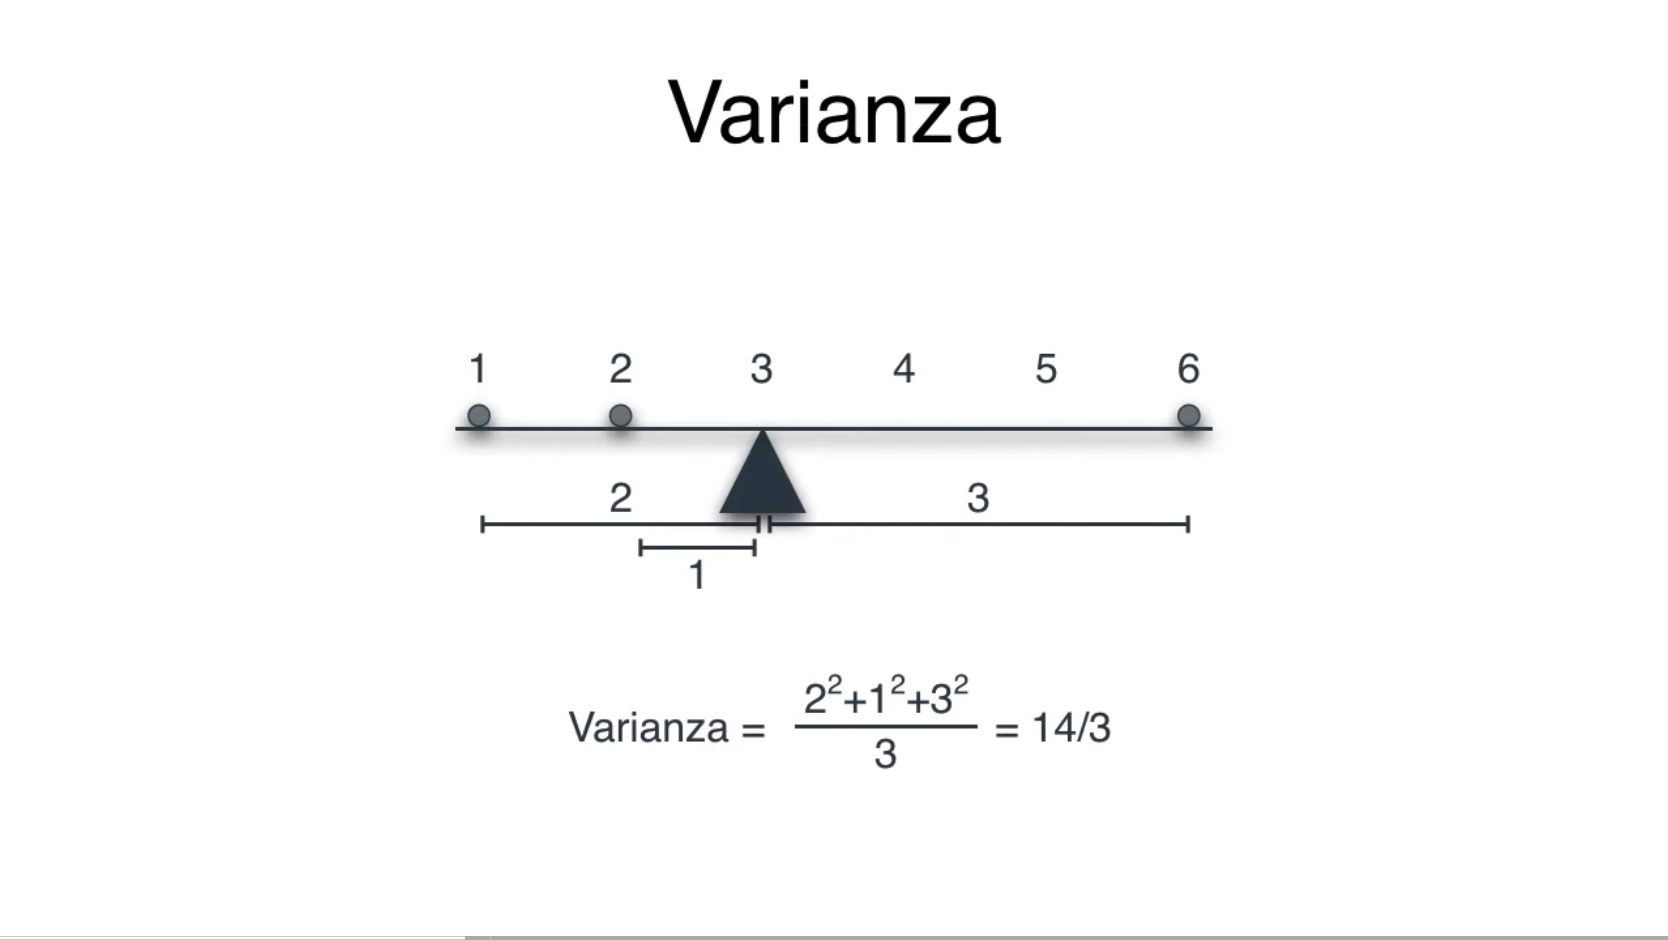
\includegraphics[width=0.9\textwidth]{PCA/IMG_3549.jpg}
			\caption{https://serrano.academy/espanol/}
		\end{figure}
	\end{block}
\end{frame}


\begin{frame}
	\frametitle{REDUCCIÓN DE DIMENSIONALIDAD}
	\begin{block}{Análisis de Componentes Principales}	
		\begin{figure}
			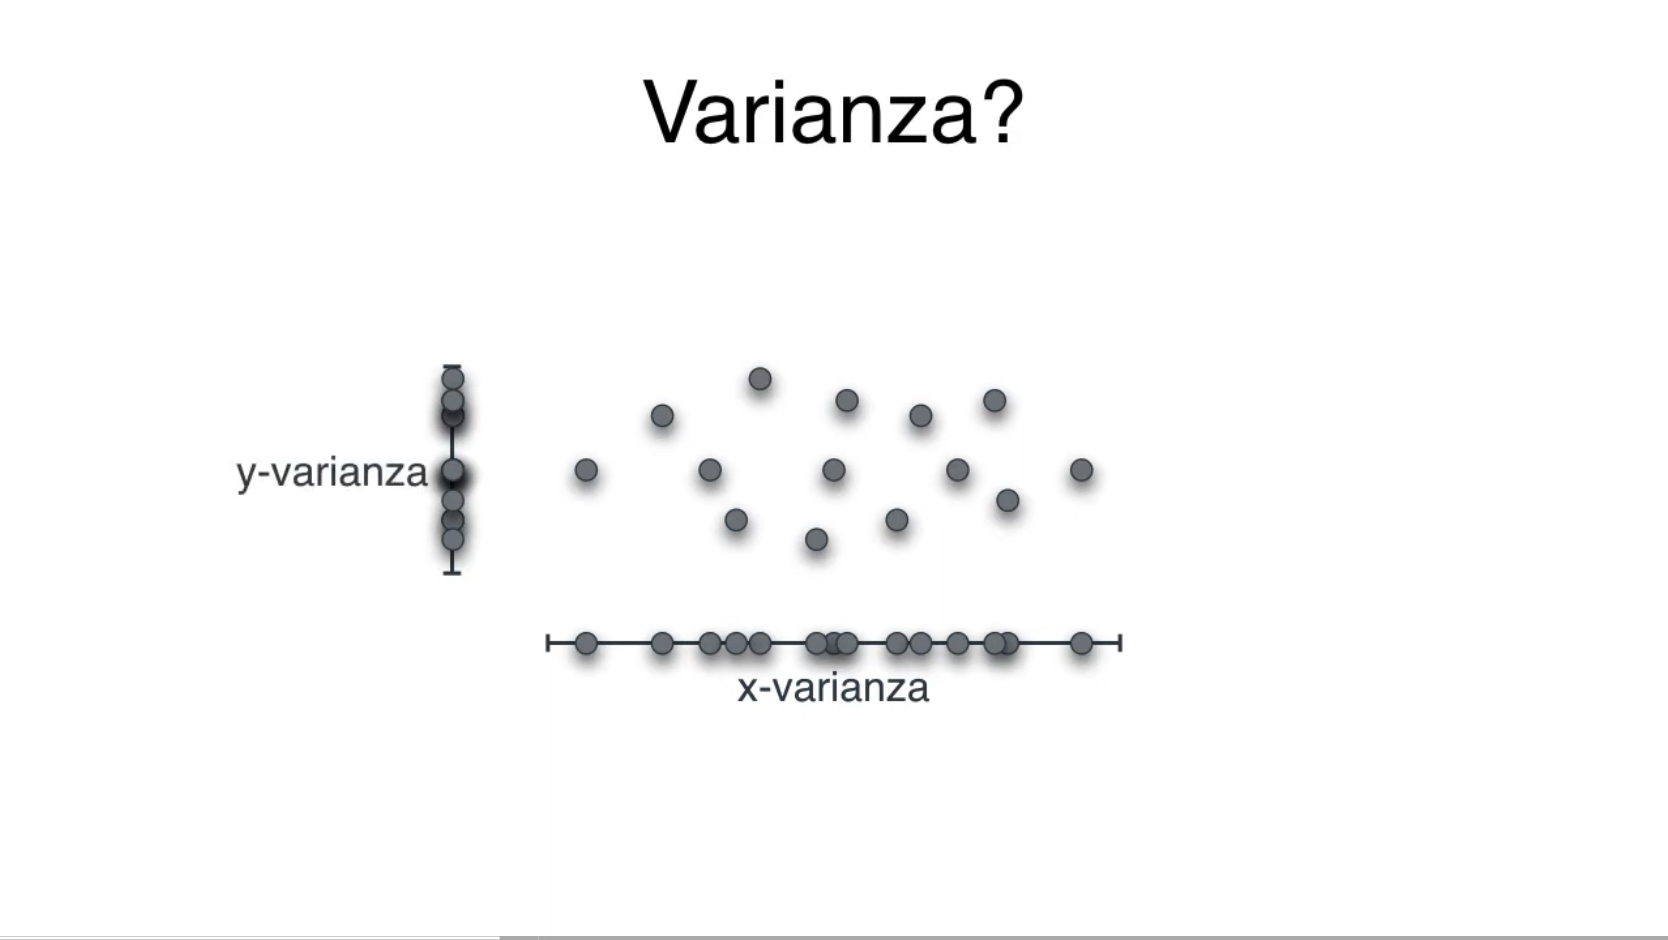
\includegraphics[width=0.9\textwidth]{PCA/IMG_3550.jpg}
			\caption{https://serrano.academy/espanol/}
		\end{figure}
	\end{block}
\end{frame}

\begin{frame}
	\frametitle{REDUCCIÓN DE DIMENSIONALIDAD}
	\begin{block}{Análisis de Componentes Principales}	
		\begin{figure}
			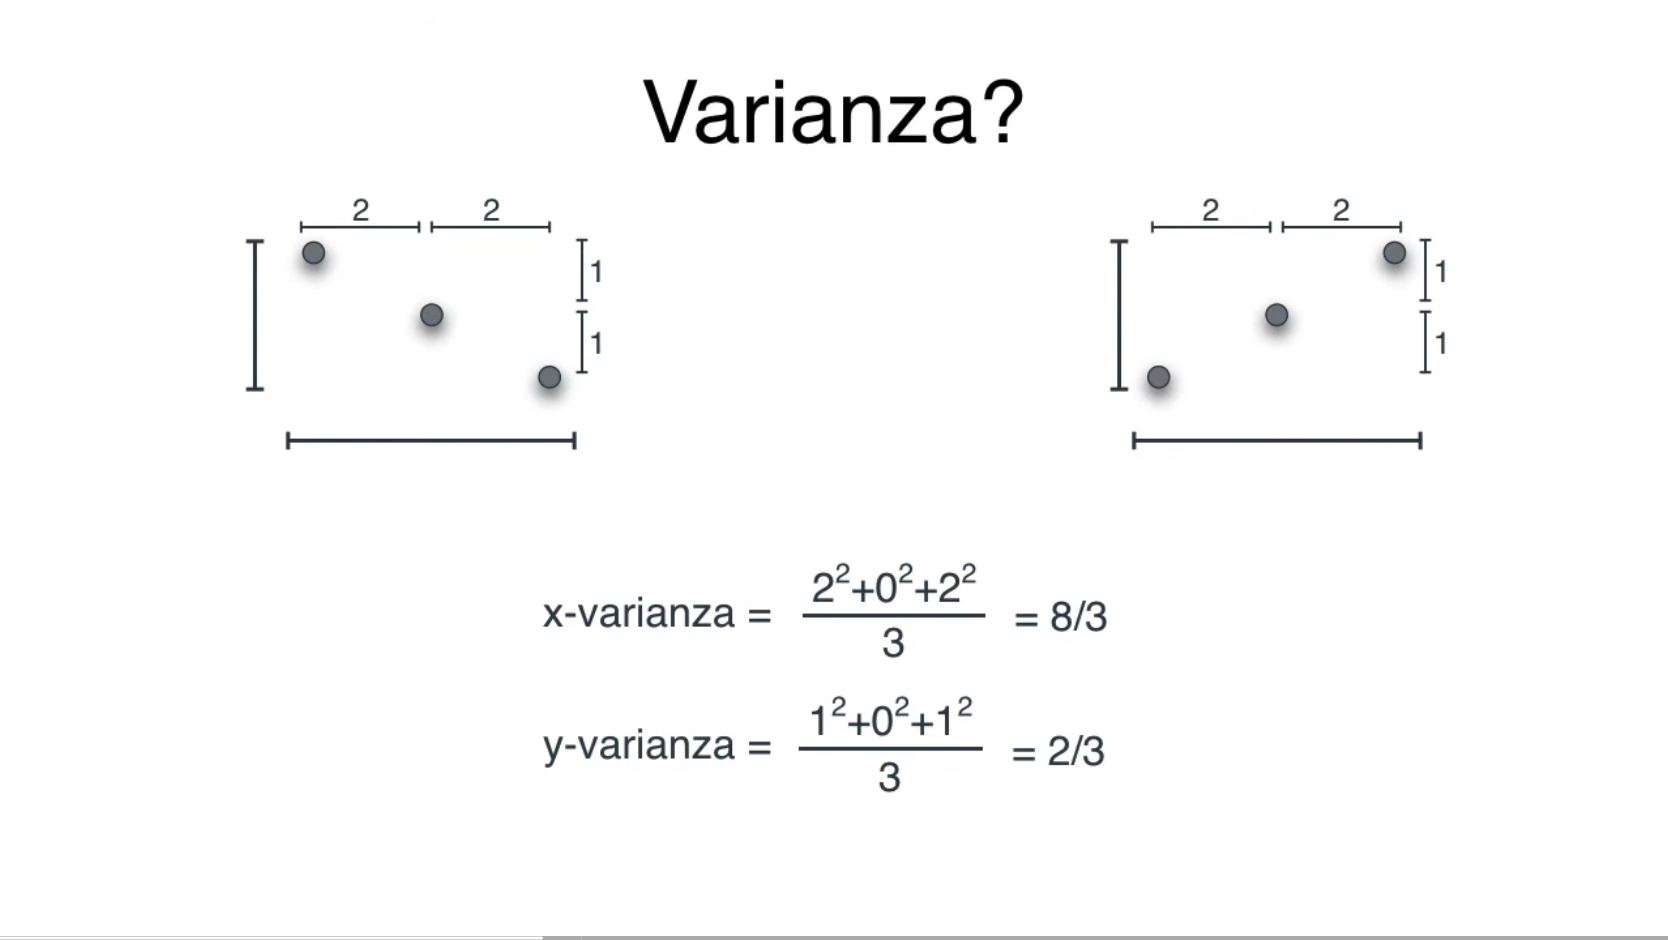
\includegraphics[width=0.9\textwidth]{PCA/IMG_3551.jpg}
			\caption{https://serrano.academy/espanol/}
		\end{figure}
	\end{block}
\end{frame}

\begin{frame}
	\frametitle{REDUCCIÓN DE DIMENSIONALIDAD}
	\begin{block}{Análisis de Componentes Principales}	
		\begin{figure}
			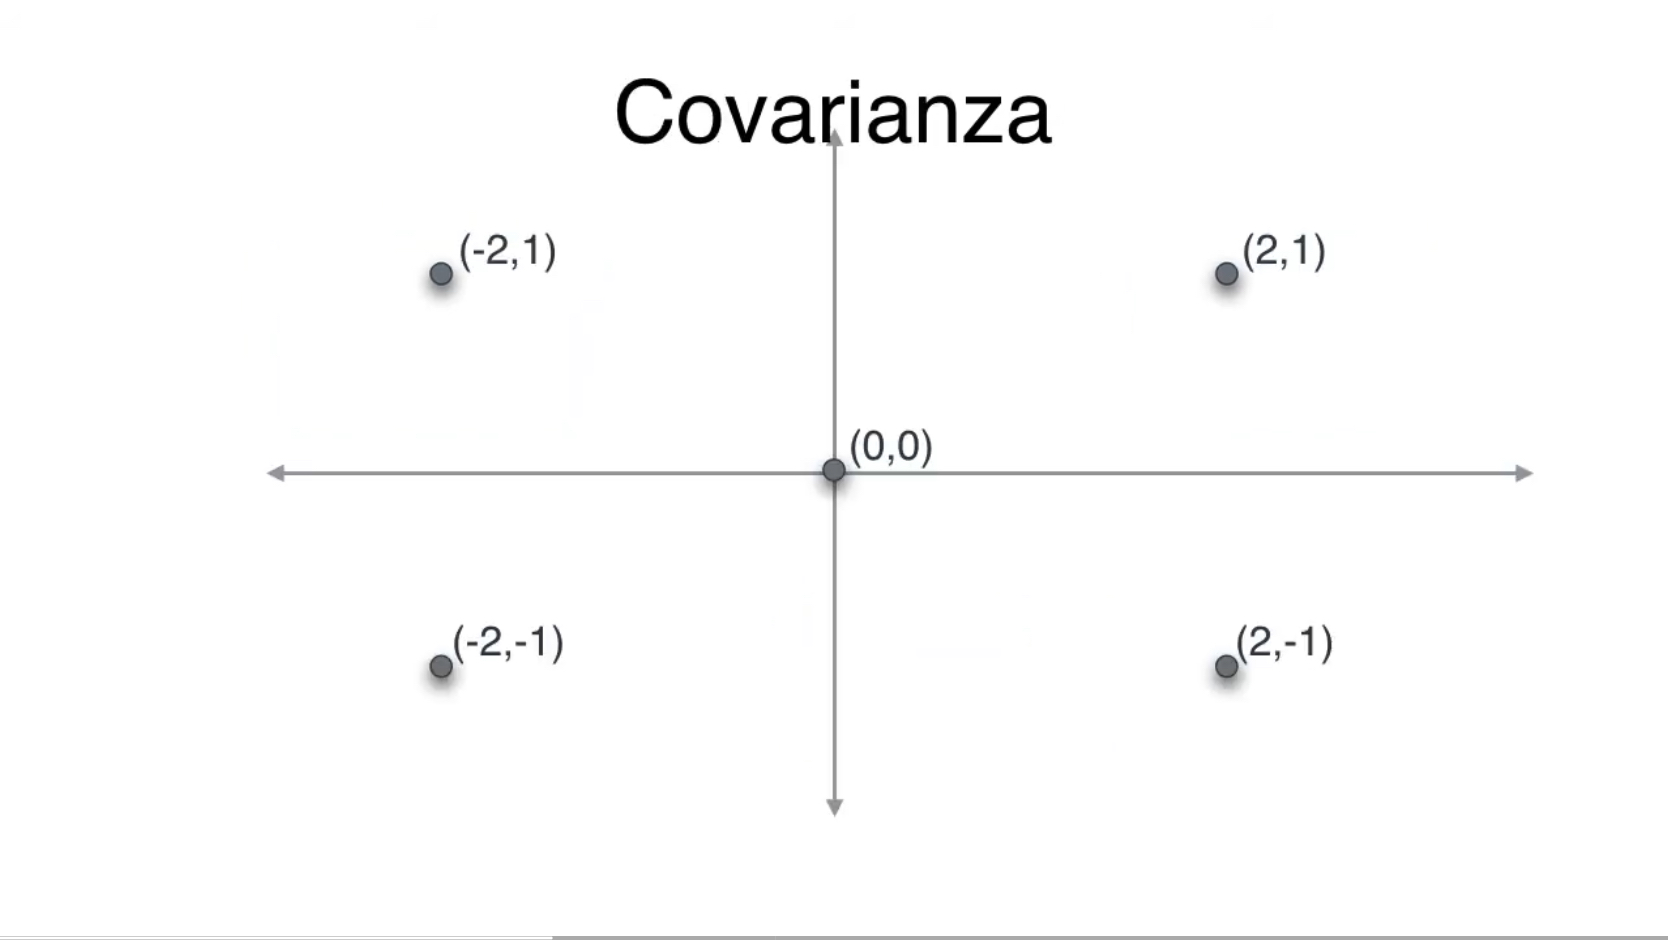
\includegraphics[width=0.9\textwidth]{PCA/IMG_3552.jpg}
			\caption{https://serrano.academy/espanol/}
		\end{figure}
	\end{block}
\end{frame}

\begin{frame}
	\frametitle{REDUCCIÓN DE DIMENSIONALIDAD}
	\begin{block}{Análisis de Componentes Principales}	
		\begin{figure}
			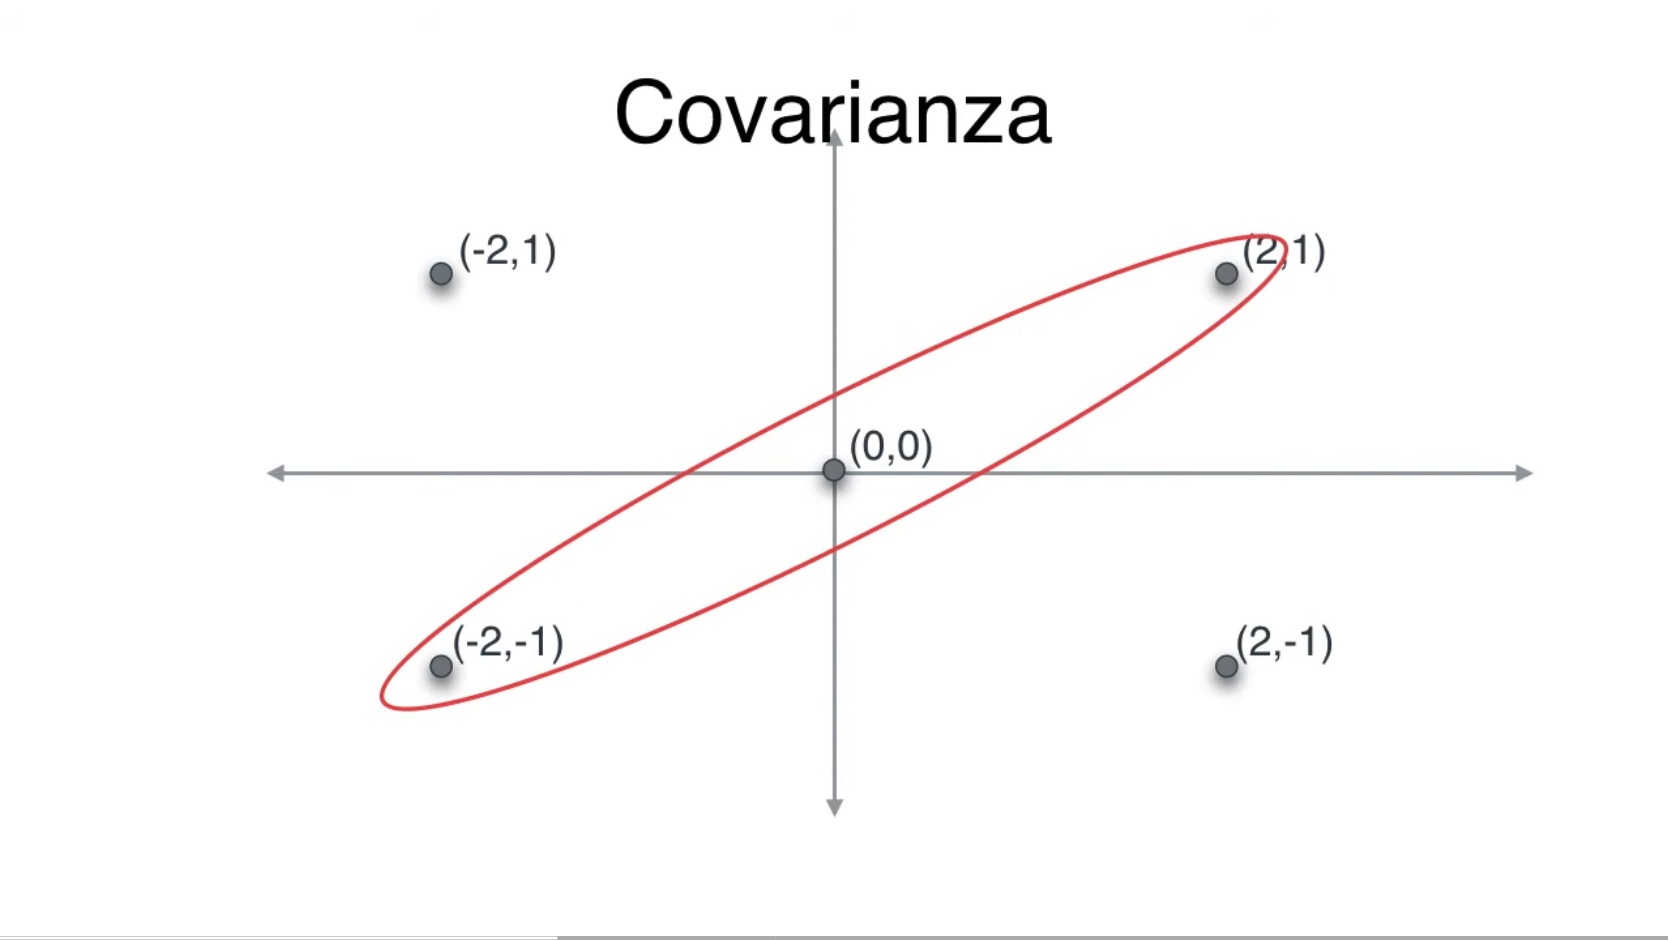
\includegraphics[width=0.9\textwidth]{PCA/IMG_3553.jpg}
			\caption{https://serrano.academy/espanol/}
		\end{figure}
	\end{block}
\end{frame}

\begin{frame}
	\frametitle{REDUCCIÓN DE DIMENSIONALIDAD}
	\begin{block}{Análisis de Componentes Principales}	
		\begin{figure}
			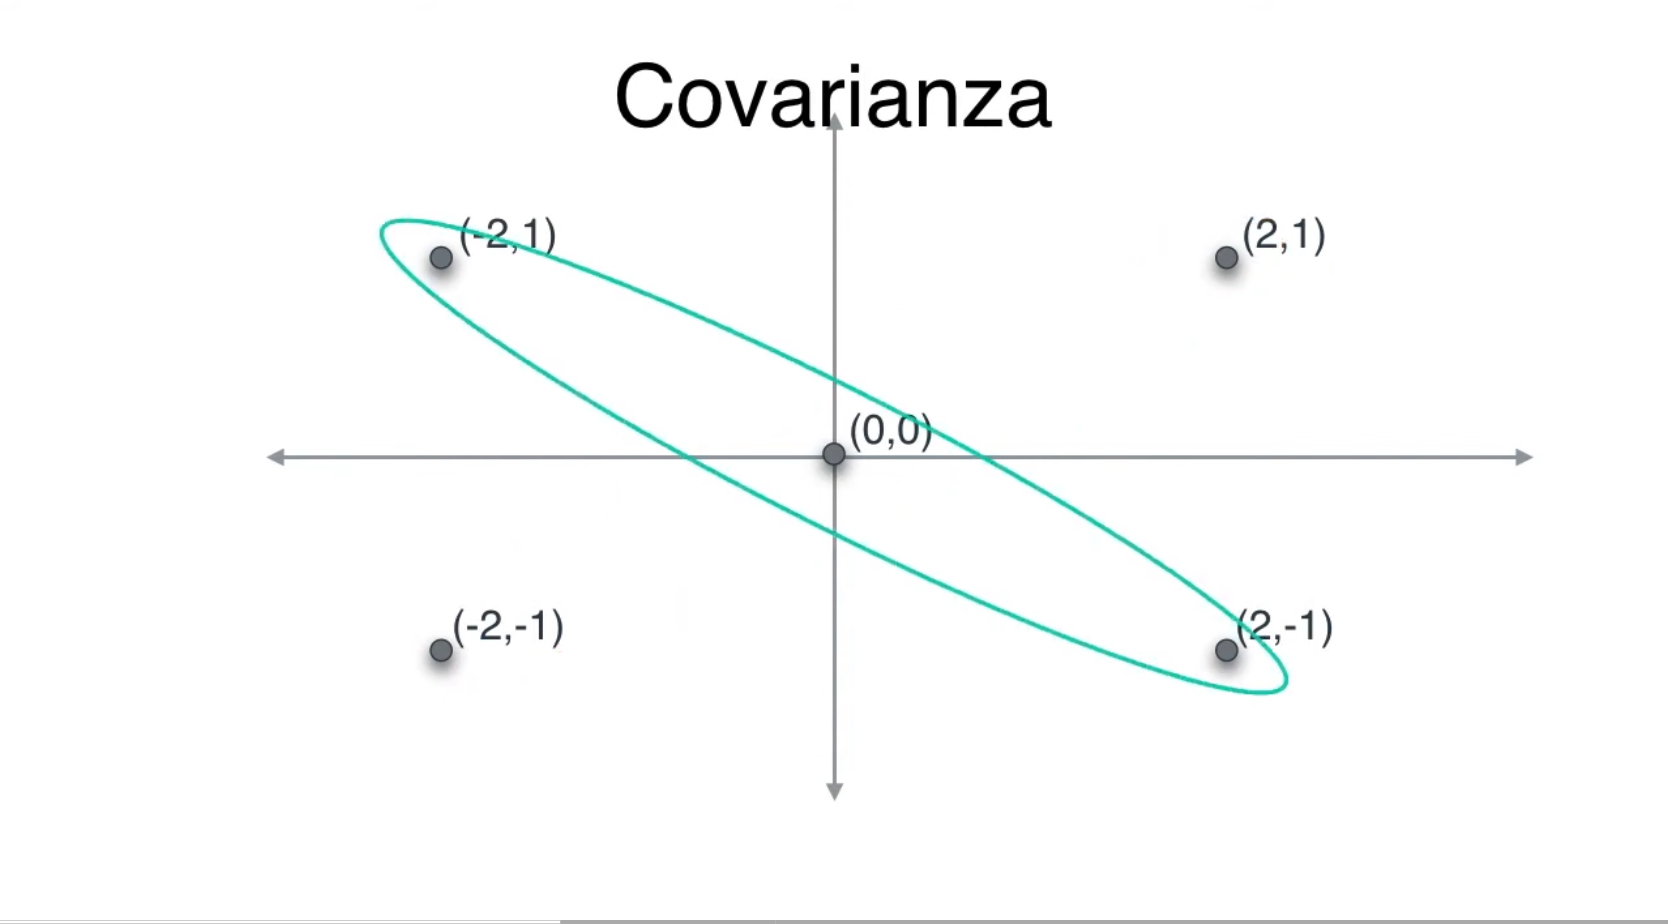
\includegraphics[width=0.9\textwidth]{PCA/IMG_3554.jpg}
			\caption{https://serrano.academy/espanol/}
		\end{figure}
	\end{block}
\end{frame}

\begin{frame}
	\frametitle{REDUCCIÓN DE DIMENSIONALIDAD}
	\begin{block}{Análisis de Componentes Principales}	
		\begin{figure}
			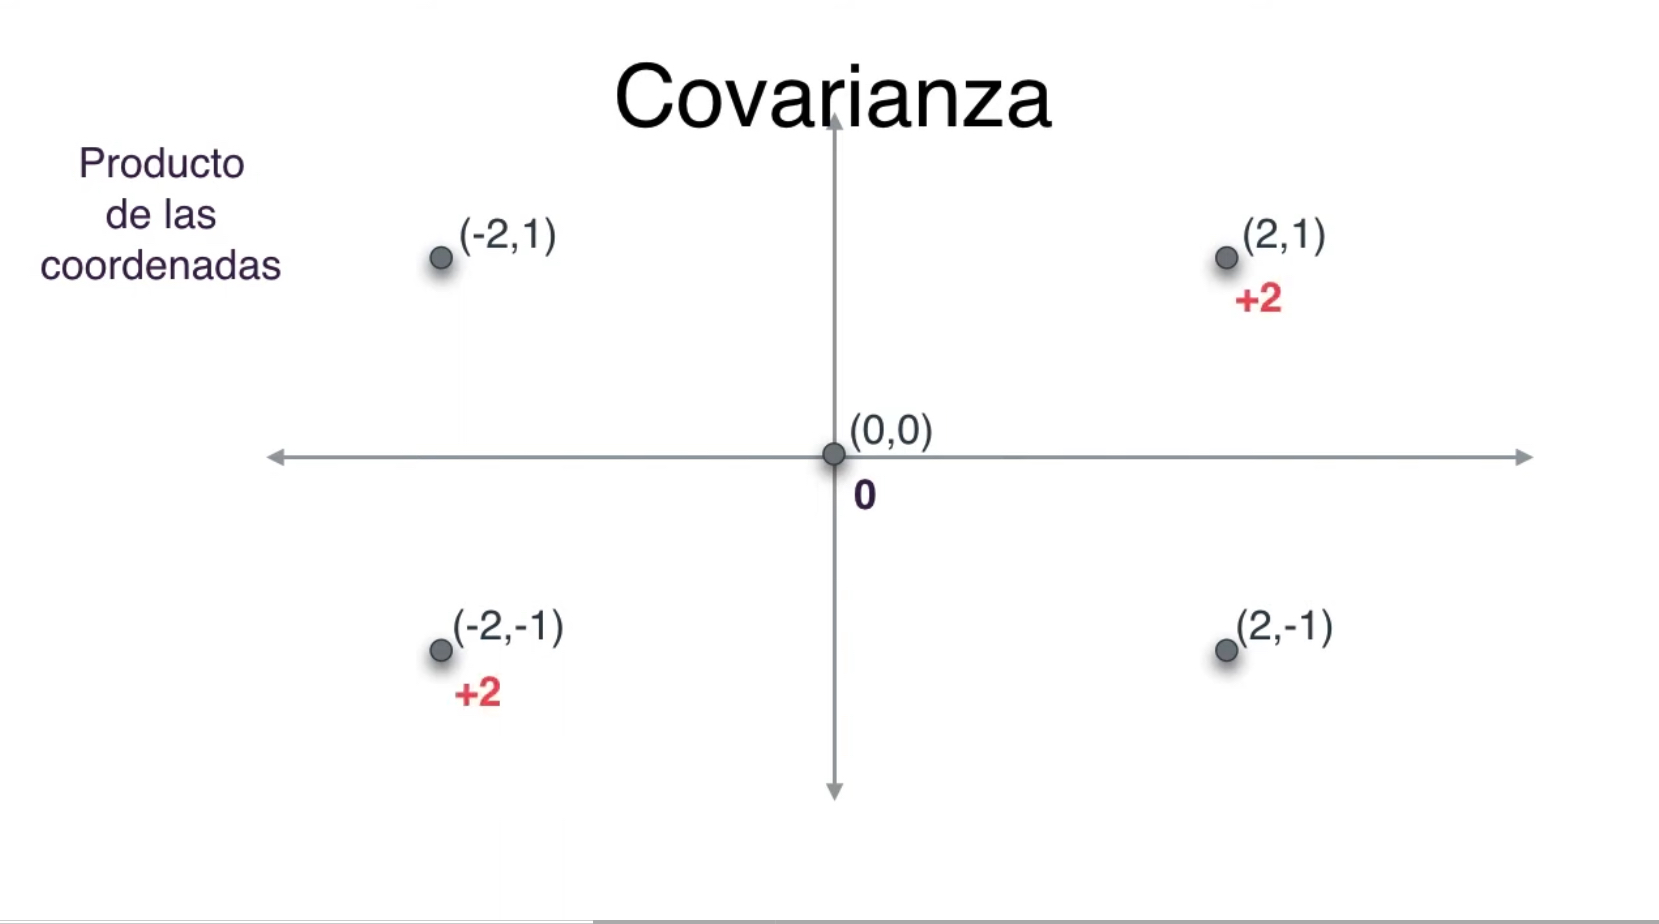
\includegraphics[width=0.9\textwidth]{PCA/IMG_3555.jpg}
			\caption{https://serrano.academy/espanol/}
		\end{figure}
	\end{block}
\end{frame}


\begin{frame}
	\frametitle{REDUCCIÓN DE DIMENSIONALIDAD}
	\begin{block}{Análisis de Componentes Principales}	
		\begin{figure}
			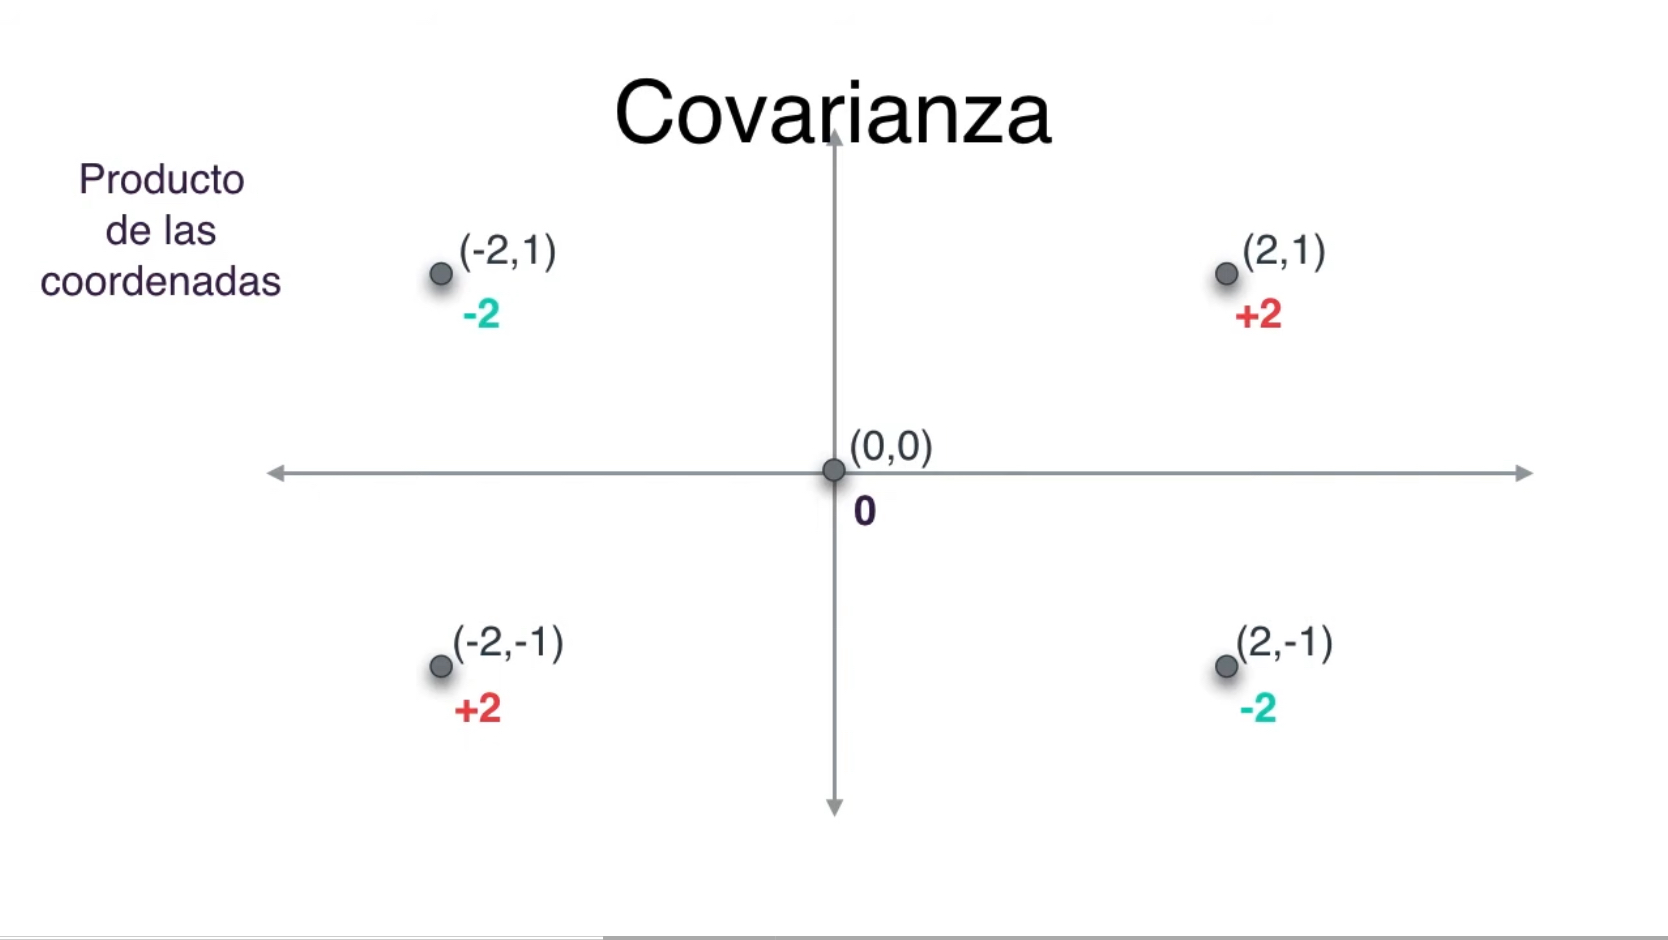
\includegraphics[width=0.9\textwidth]{PCA/IMG_3556.jpg}
			\caption{https://serrano.academy/espanol/}
		\end{figure}
	\end{block}
\end{frame}

\begin{frame}
	\frametitle{REDUCCIÓN DE DIMENSIONALIDAD}
	\begin{block}{Análisis de Componentes Principales}	
		\begin{figure}
			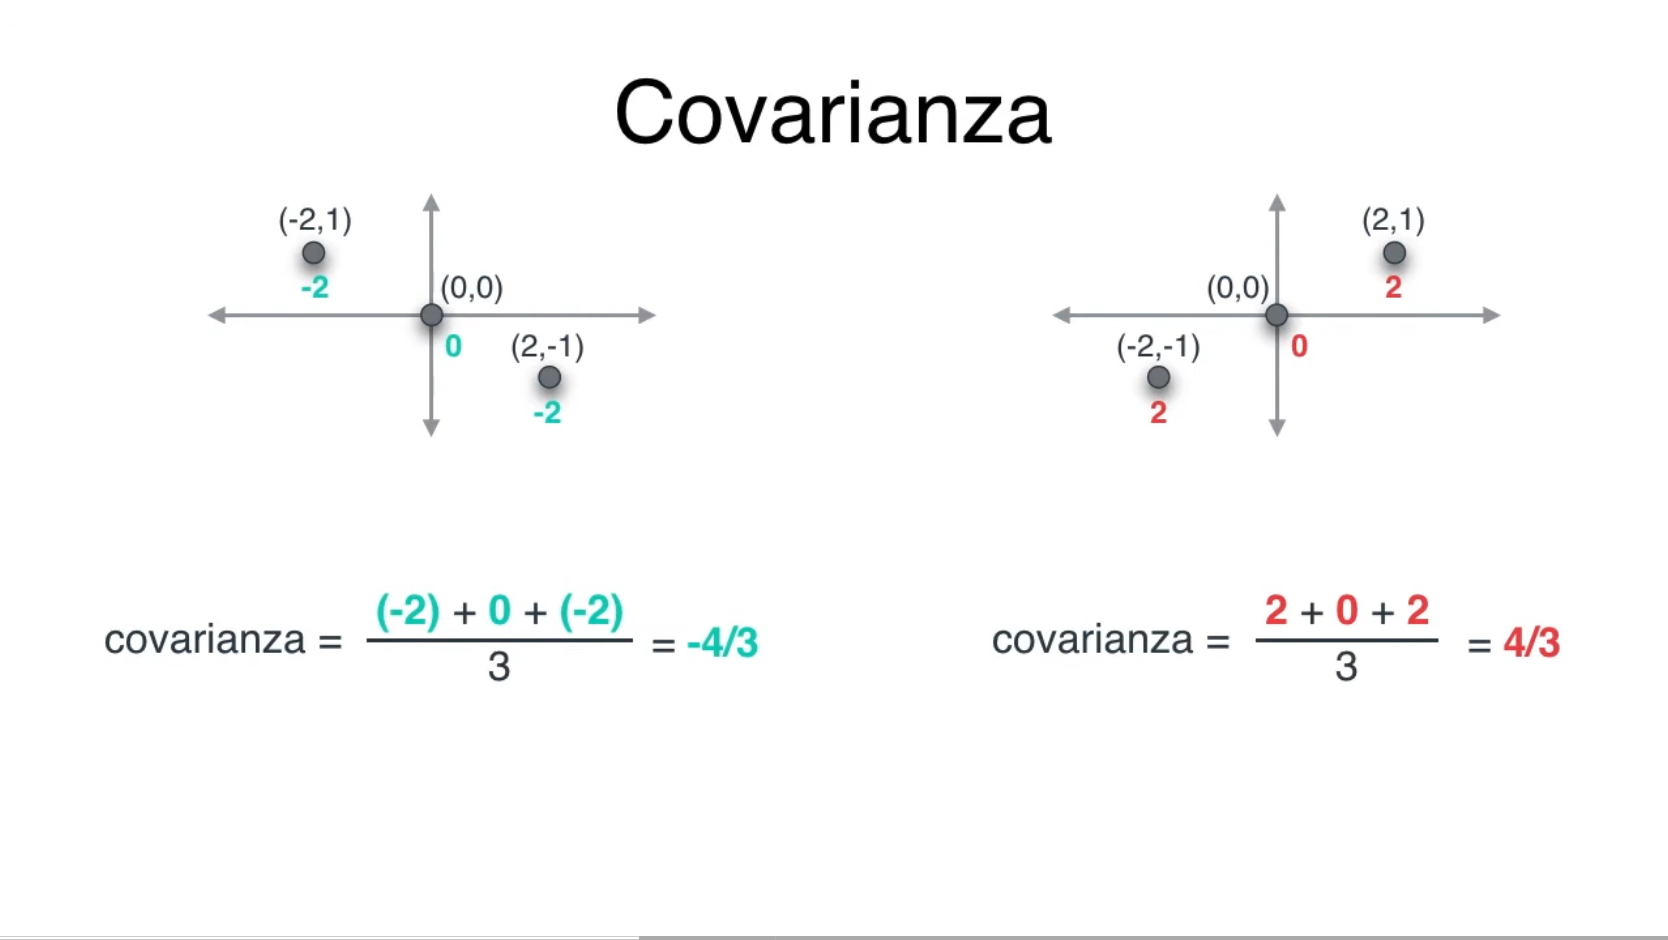
\includegraphics[width=0.9\textwidth]{PCA/IMG_3557.jpg}
			\caption{https://serrano.academy/espanol/}
		\end{figure}
	\end{block}
\end{frame}

\begin{frame}
	\frametitle{REDUCCIÓN DE DIMENSIONALIDAD}
	\begin{block}{Análisis de Componentes Principales}	
		\begin{figure}
			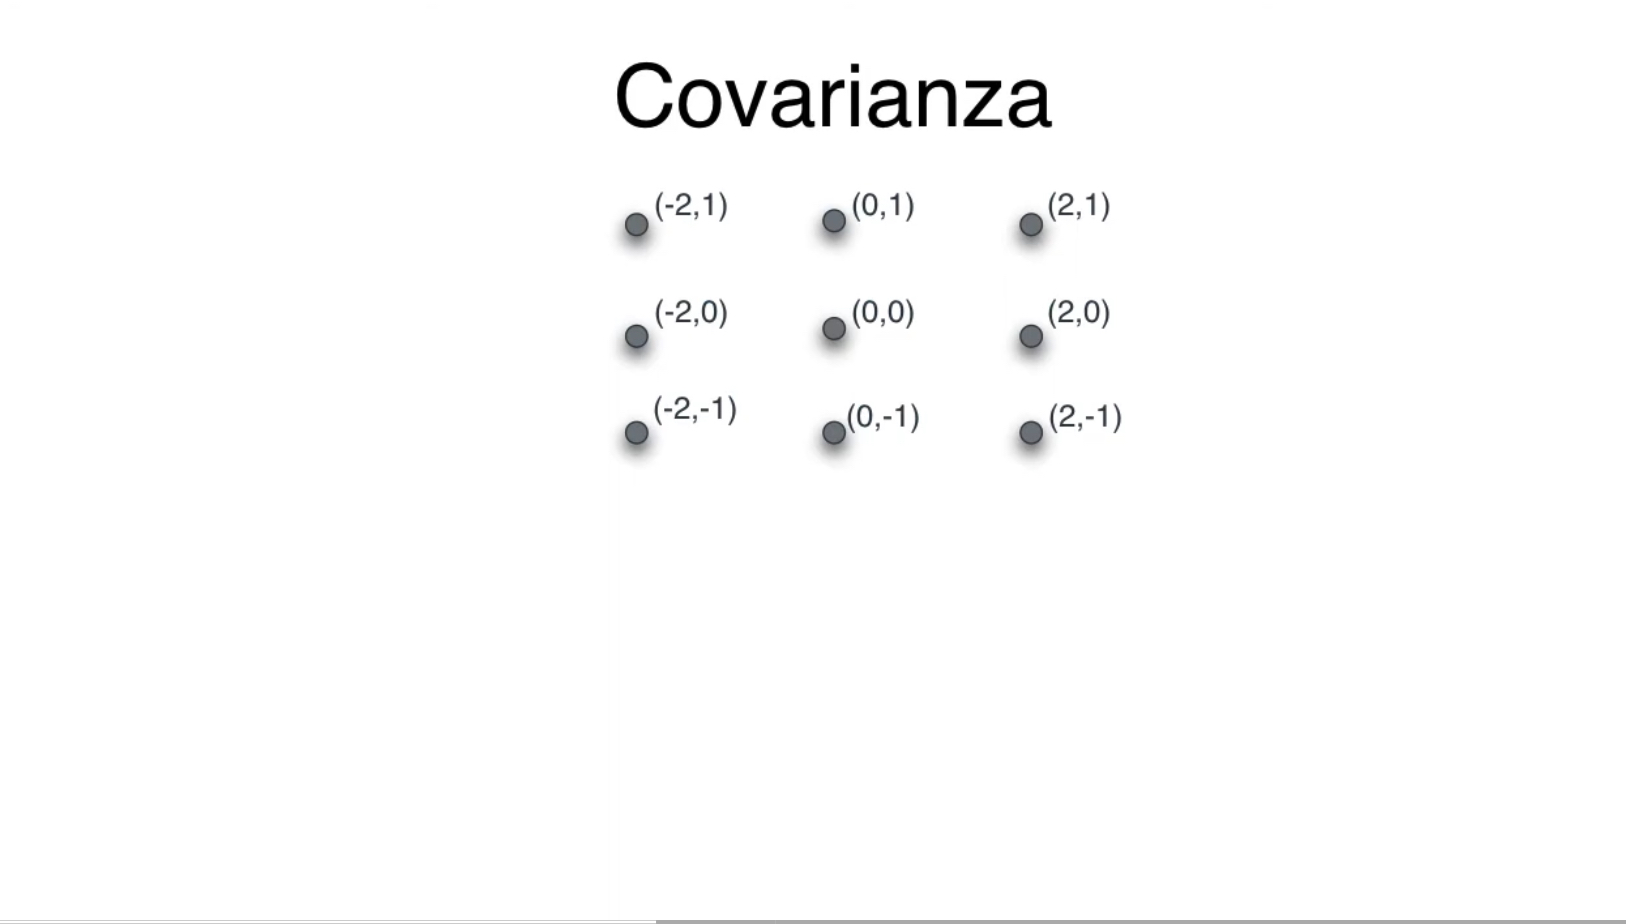
\includegraphics[width=0.9\textwidth]{PCA/IMG_3558.jpg}
			\caption{https://serrano.academy/espanol/}
		\end{figure}
	\end{block}
\end{frame}

\begin{frame}
	\frametitle{REDUCCIÓN DE DIMENSIONALIDAD}
	\begin{block}{Análisis de Componentes Principales}	
		\begin{figure}
			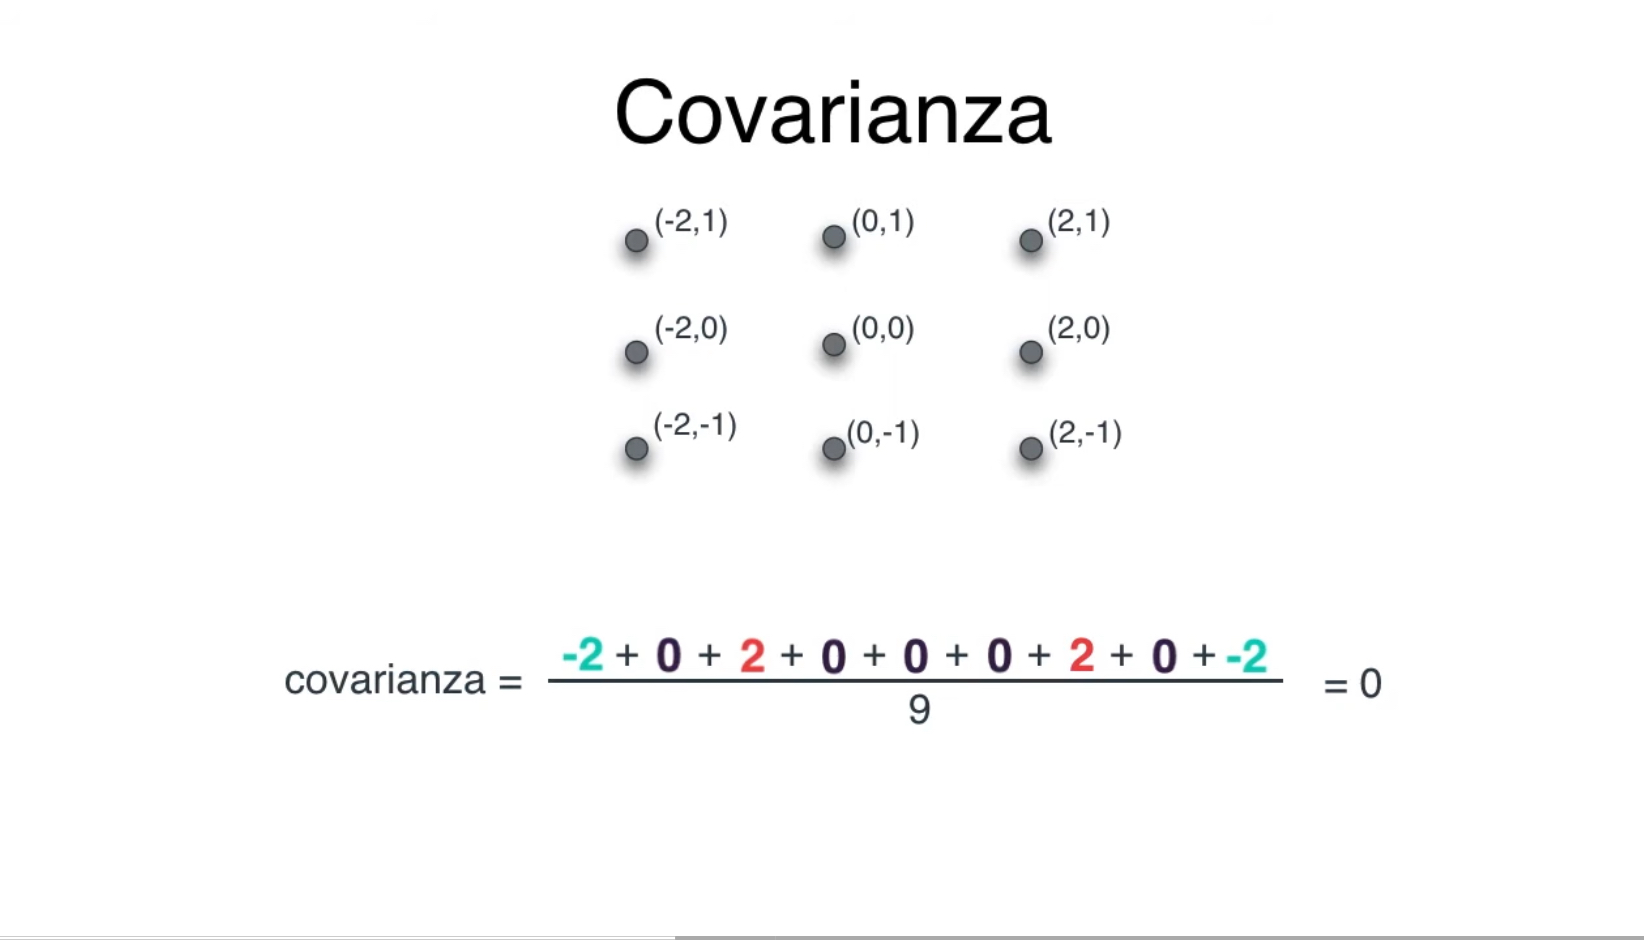
\includegraphics[width=0.9\textwidth]{PCA/IMG_3559.jpg}
			\caption{https://serrano.academy/espanol/}
		\end{figure}
	\end{block}
\end{frame}

\begin{frame}
	\frametitle{REDUCCIÓN DE DIMENSIONALIDAD}
	\begin{block}{Análisis de Componentes Principales}	
		\begin{figure}
			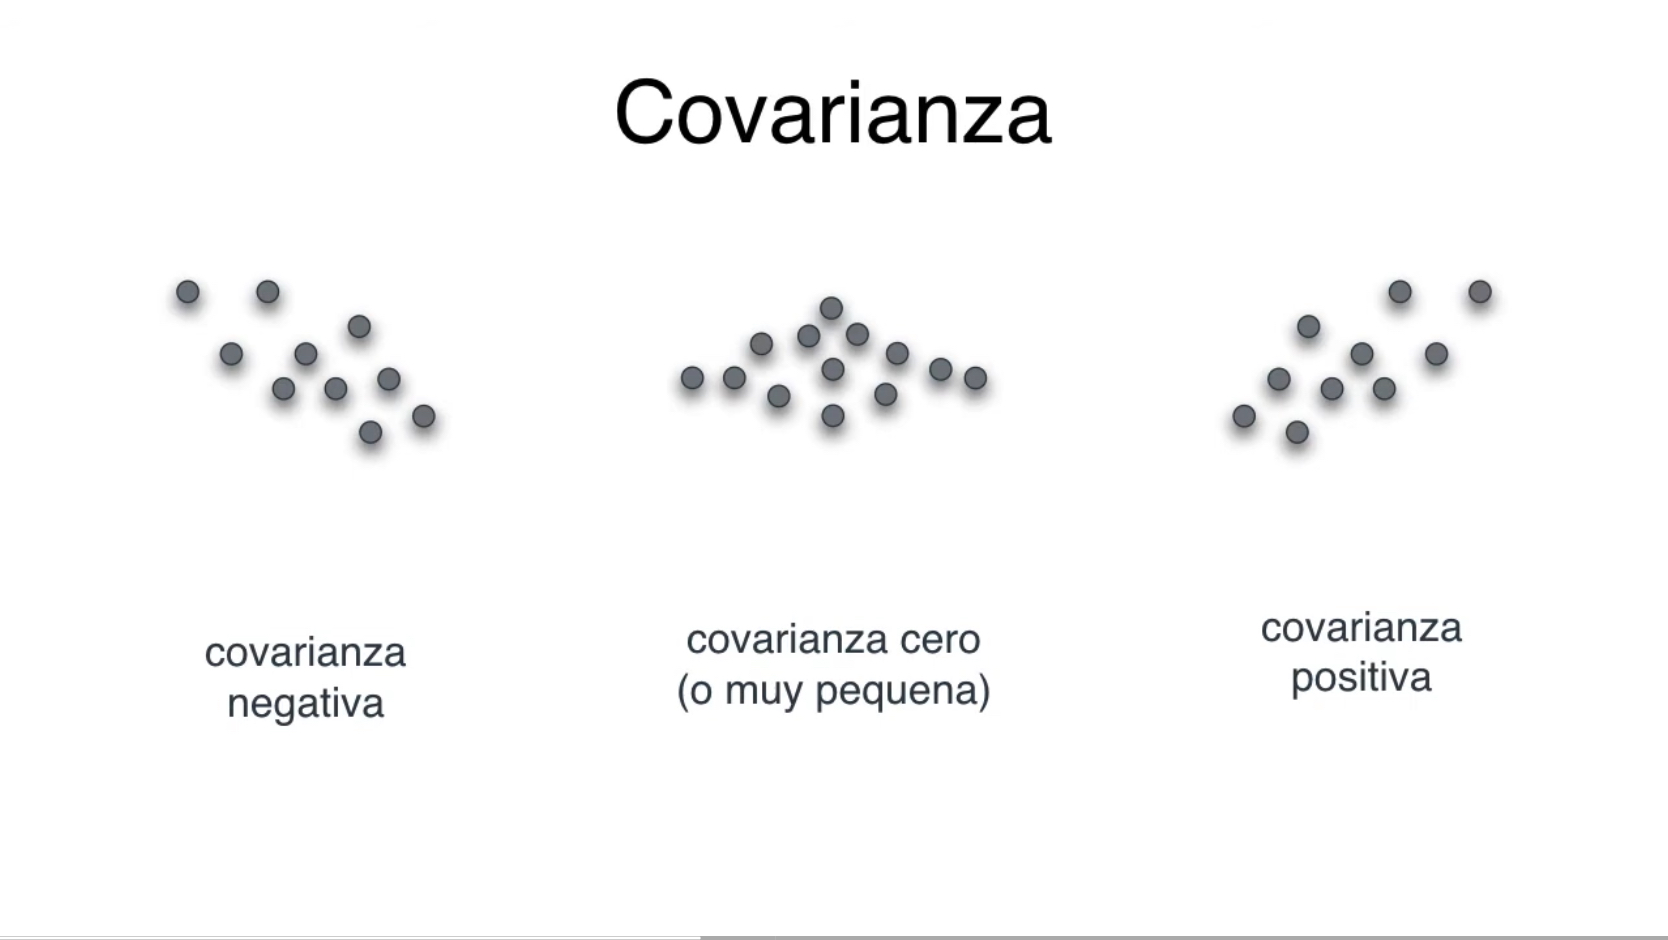
\includegraphics[width=0.9\textwidth]{PCA/IMG_3560.jpg}
			\caption{https://serrano.academy/espanol/}
		\end{figure}
	\end{block}
\end{frame}


\begin{frame}
	\frametitle{REDUCCIÓN DE DIMENSIONALIDAD}
\begin{block}{Análisis de Componentes Principales}	
\textbf{Valores y vectores propios}
\end{block}
\end{frame}

\begin{frame}
\frametitle{REDUCCIÓN DE DIMENSIONALIDAD}
\begin{block}{Análisis de Componentes Principales}	
	\begin{figure}
		
\includegraphics[width=0.9\textwidth]{PCA/IMG_3562.jpg}
		\caption{https://serrano.academy/espanol/}
	\end{figure}
\end{block}
\end{frame}

\begin{frame}
\frametitle{REDUCCIÓN DE DIMENSIONALIDAD}
\begin{block}{Análisis de Componentes Principales}	
	\begin{figure}
		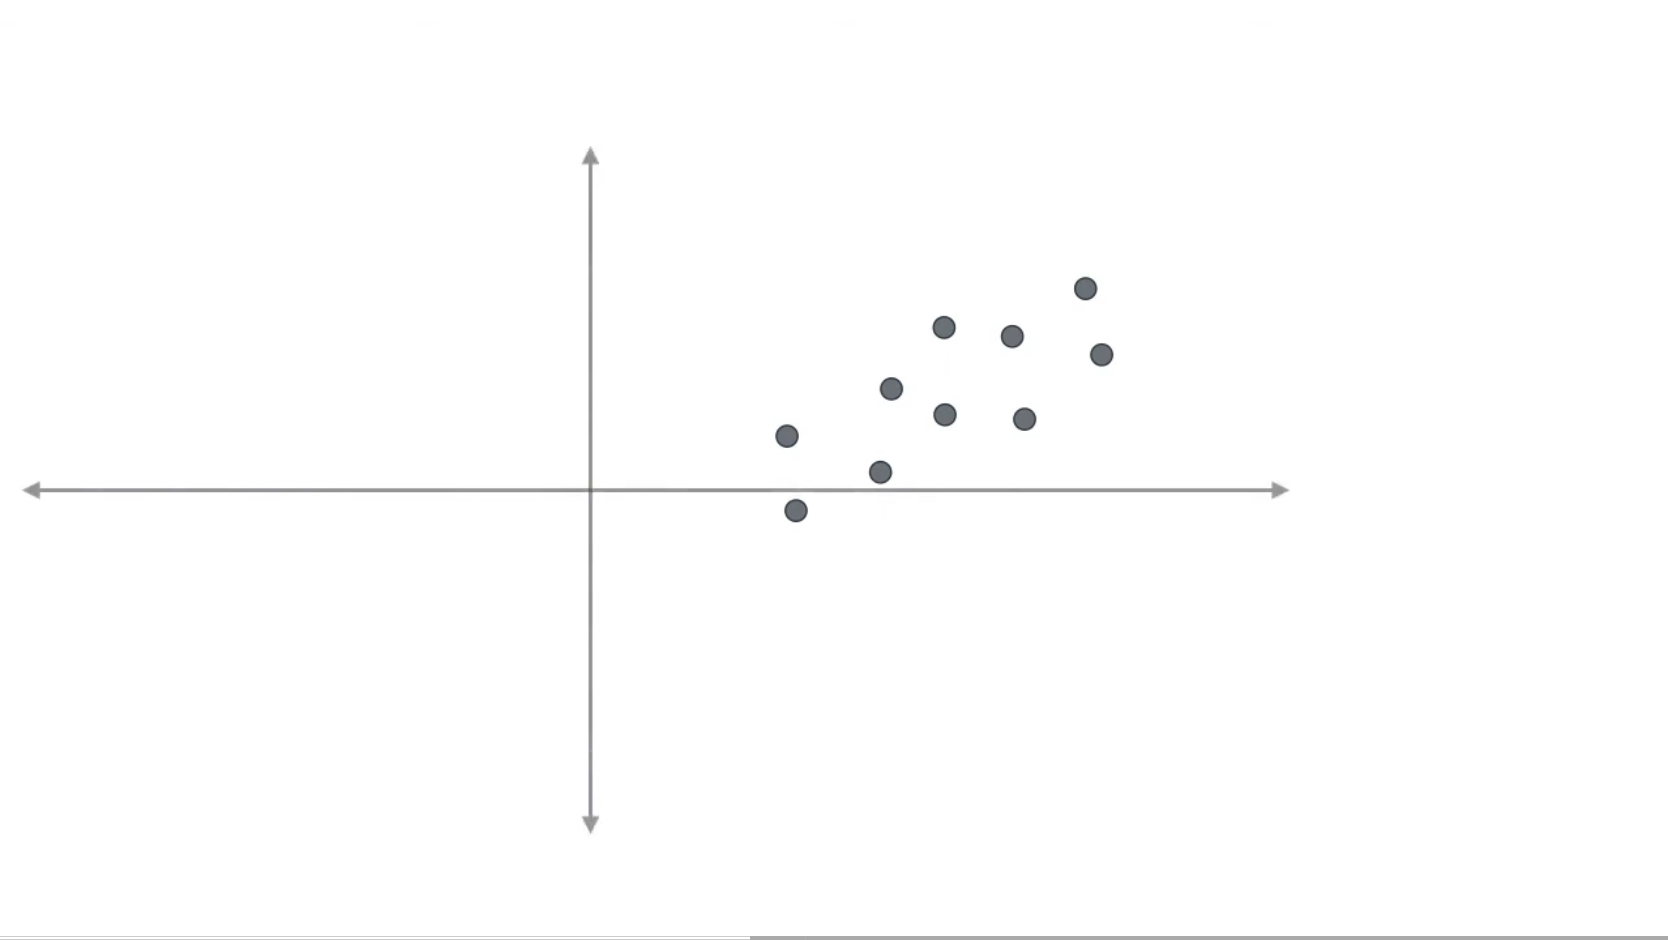
\includegraphics[width=0.9\textwidth]{PCA/IMG_3563.jpg}
		\caption{https://serrano.academy/espanol/}
	\end{figure}
\end{block}
\end{frame}

\begin{frame}
\frametitle{REDUCCIÓN DE DIMENSIONALIDAD}
\begin{block}{Análisis de Componentes Principales}	
	\begin{figure}
		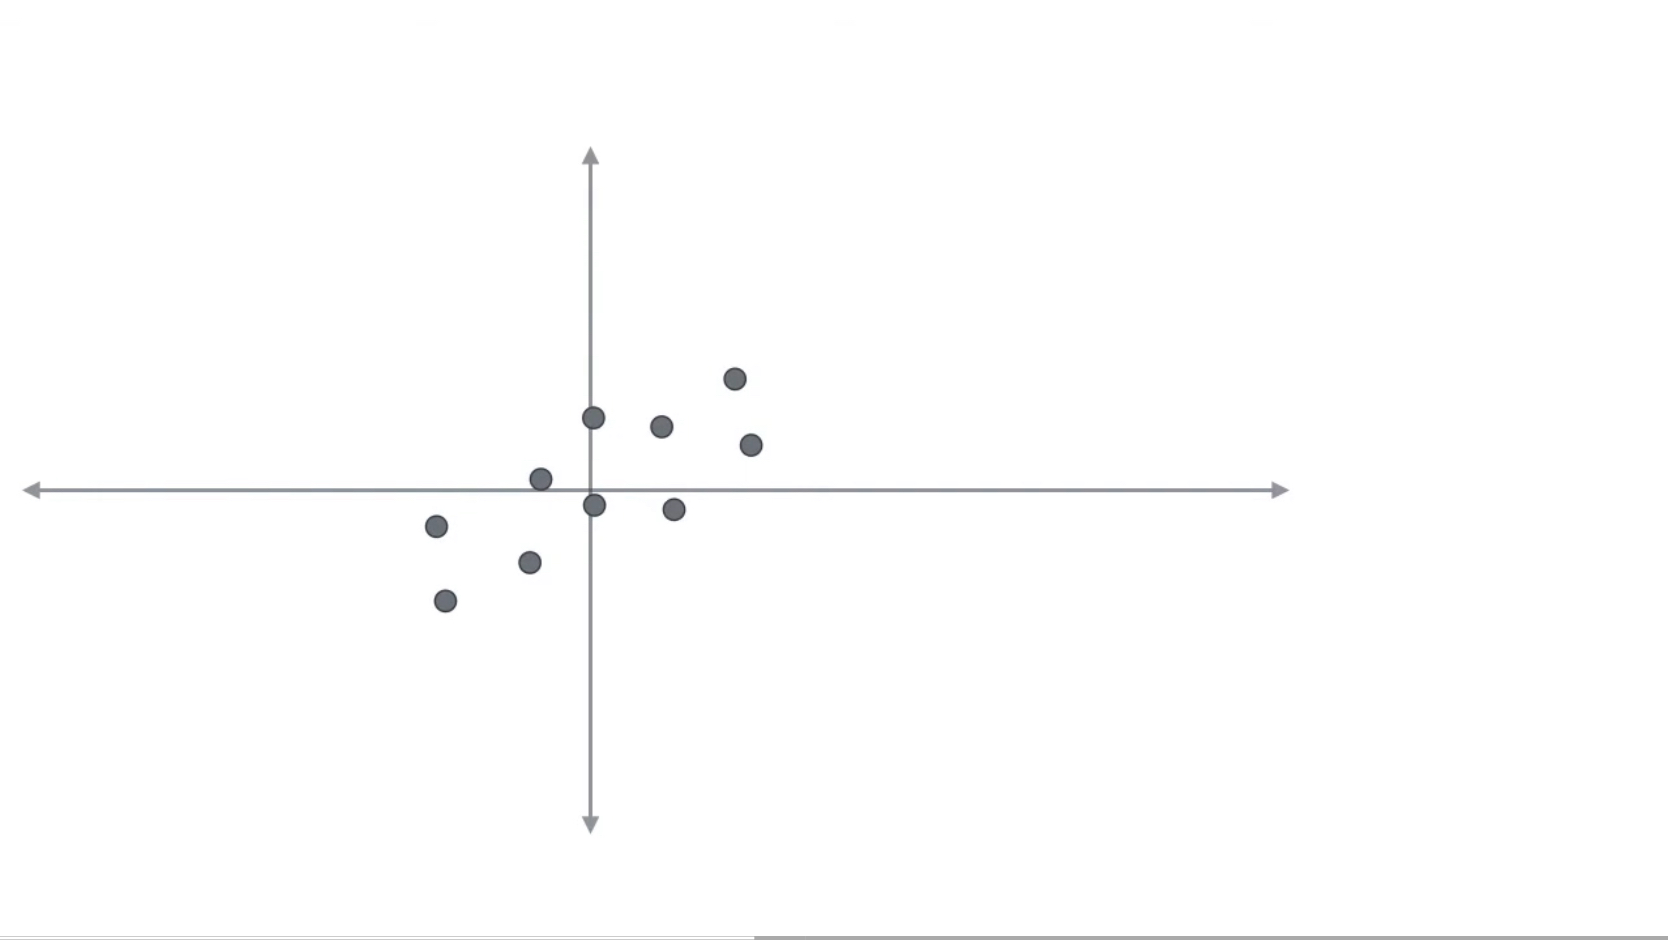
\includegraphics[width=0.9\textwidth]{PCA/IMG_3564.jpg}
		\caption{https://serrano.academy/espanol/}
	\end{figure}
\end{block}
\end{frame}

\begin{frame}
\frametitle{REDUCCIÓN DE DIMENSIONALIDAD}
\begin{block}{Análisis de Componentes Principales}	
	\begin{figure}
		\includegraphics[width=0.9\textwidth]{PCA/IMG_3565.jpg}
		\caption{https://serrano.academy/espanol/}
	\end{figure}
\end{block}
\end{frame}


\begin{frame}
\frametitle{REDUCCIÓN DE DIMENSIONALIDAD}
\begin{block}{Análisis de Componentes Principales}	
	\begin{figure}
		\includegraphics[width=0.9\textwidth]{PCA/IMG_3566.jpg}
		\caption{https://serrano.academy/espanol/}
	\end{figure}
\end{block}
\end{frame}

\begin{frame}
\frametitle{REDUCCIÓN DE DIMENSIONALIDAD}
\begin{block}{Análisis de Componentes Principales}	
	\begin{figure}
		\includegraphics[width=0.9\textwidth]{PCA/IMG_3567.jpg}
		\caption{https://serrano.academy/espanol/}
	\end{figure}
\end{block}
\end{frame}

\begin{frame}
\frametitle{REDUCCIÓN DE DIMENSIONALIDAD}
\begin{block}{Análisis de Componentes Principales}	
	\begin{figure}
		\includegraphics[width=0.9\textwidth]{PCA/IMG_3568.jpg}
		\caption{https://serrano.academy/espanol/}
	\end{figure}
\end{block}
\end{frame}

\begin{frame}
\frametitle{REDUCCIÓN DE DIMENSIONALIDAD}
\begin{block}{Análisis de Componentes Principales}	
	\begin{figure}
		\includegraphics[width=0.9\textwidth]{PCA/IMG_3569.jpg}
		\caption{https://serrano.academy/espanol/}
	\end{figure}
\end{block}
\end{frame}

\begin{frame}
\frametitle{REDUCCIÓN DE DIMENSIONALIDAD}
\begin{block}{Análisis de Componentes Principales}	
	\begin{figure}
		\includegraphics[width=0.9\textwidth]{PCA/IMG_3570.jpg}
		\caption{https://serrano.academy/espanol/}
	\end{figure}
\end{block}
\end{frame}


\begin{frame}
	\frametitle{REDUCCIÓN DE DIMENSIONALIDAD}
	\begin{block}{Análisis de Componentes Principales}	
		\begin{figure}
			\includegraphics[width=0.9\textwidth]{PCA/IMG_3571.jpg}
			\caption{https://serrano.academy/espanol/}
		\end{figure}
	\end{block}
\end{frame}

\begin{frame}
	\frametitle{REDUCCIÓN DE DIMENSIONALIDAD}
	\begin{block}{Análisis de Componentes Principales}	
		\begin{figure}
			\includegraphics[width=0.9\textwidth]{PCA/IMG_3572.jpg}
			\caption{https://serrano.academy/espanol/}
		\end{figure}
	\end{block}
\end{frame}

\begin{frame}
	\frametitle{REDUCCIÓN DE DIMENSIONALIDAD}
	\begin{block}{Análisis de Componentes Principales}	
		\begin{figure}
			\includegraphics[width=0.9\textwidth]{PCA/IMG_3573.jpg}
			\caption{https://serrano.academy/espanol/}
		\end{figure}
	\end{block}
\end{frame}

\begin{frame}
	\frametitle{REDUCCIÓN DE DIMENSIONALIDAD}
	\begin{block}{Análisis de Componentes Principales}	
		\begin{figure}
			\includegraphics[width=0.9\textwidth]{PCA/IMG_3574.jpg}
			\caption{https://serrano.academy/espanol/}
		\end{figure}
	\end{block}
\end{frame}

\begin{frame}
	\frametitle{REDUCCIÓN DE DIMENSIONALIDAD}
	\begin{block}{Análisis de Componentes Principales}	
		\begin{figure}
			\includegraphics[width=0.9\textwidth]{PCA/IMG_3575.jpg}
			\caption{https://serrano.academy/espanol/}
		\end{figure}
	\end{block}
\end{frame}


\begin{frame}
	\frametitle{REDUCCIÓN DE DIMENSIONALIDAD}
	\begin{block}{Análisis de Componentes Principales}	
		\begin{figure}
			\includegraphics[width=0.9\textwidth]{PCA/IMG_3576.jpg}
			\caption{https://serrano.academy/espanol/}
		\end{figure}
	\end{block}
\end{frame}



\begin{frame}
	\frametitle{REDUCCIÓN DE DIMENSIONALIDAD}
	\begin{block}{Análisis de Componentes Principales}	
		\begin{figure}
			\includegraphics[width=0.9\textwidth]{PCA/IMG_3578.jpg}
			\caption{https://serrano.academy/espanol/}
		\end{figure}
	\end{block}
\end{frame}

\begin{frame}
	\frametitle{REDUCCIÓN DE DIMENSIONALIDAD}
	\begin{block}{Análisis de Componentes Principales}	
		\begin{figure}
			\includegraphics[width=0.9\textwidth]{PCA/IMG_3579.jpg}
			\caption{https://serrano.academy/espanol/}
		\end{figure}
	\end{block}
\end{frame}

\begin{frame}
	\frametitle{REDUCCIÓN DE DIMENSIONALIDAD}
	\begin{block}{Análisis de Componentes Principales}	
		\begin{figure}
			\includegraphics[width=0.9\textwidth]{PCA/IMG_3580.jpg}
			\caption{https://serrano.academy/espanol/}
		\end{figure}
	\end{block}
\end{frame}

\begin{frame}
	\frametitle{REDUCCIÓN DE DIMENSIONALIDAD}
	\begin{block}{Análisis de Componentes Principales}	
		\begin{figure}
			\includegraphics[width=0.9\textwidth]{PCA/IMG_3581.jpg}
			\caption{https://serrano.academy/espanol/}
		\end{figure}
	\end{block}
\end{frame}

\begin{frame}
	\frametitle{REDUCCIÓN DE DIMENSIONALIDAD}
	\begin{block}{Análisis de Componentes Principales}	
		\begin{figure}
			\includegraphics[width=0.9\textwidth]{PCA/IMG_3582.jpg}
			\caption{https://serrano.academy/espanol/}
		\end{figure}
	\end{block}
\end{frame}

\begin{frame}
	\frametitle{REDUCCIÓN DE DIMENSIONALIDAD}
	\begin{block}{Análisis de Componentes Principales}	
		\begin{figure}
			\includegraphics[width=0.9\textwidth]{PCA/IMG_3583.jpg}
			\caption{https://serrano.academy/espanol/}
		\end{figure}
	\end{block}
\end{frame}

\begin{frame}
	\frametitle{REDUCCIÓN DE DIMENSIONALIDAD}
	\begin{block}{Análisis de Componentes Principales}	
		\begin{figure}
			\includegraphics[width=0.9\textwidth]{PCA/IMG_3584.jpg}
			\caption{https://serrano.academy/espanol/}
		\end{figure}
	\end{block}
\end{frame}

\begin{frame}
	\frametitle{REDUCCIÓN DE DIMENSIONALIDAD}
	\begin{block}{Análisis de Componentes Principales}	
		\begin{figure}
			\includegraphics[width=0.9\textwidth]{PCA/IMG_3585.jpg}
			\caption{https://serrano.academy/espanol/}
		\end{figure}
	\end{block}
\end{frame}


\begin{frame}
	\frametitle{REDUCCIÓN DE DIMENSIONALIDAD}
	\begin{block}{Análisis de Componentes Principales}	
		\begin{figure}
			\includegraphics[width=0.9\textwidth]{PCA/IMG_3586.jpg}
			\caption{https://serrano.academy/espanol/}
		\end{figure}
	\end{block}
\end{frame}

\begin{frame}
	\frametitle{REDUCCIÓN DE DIMENSIONALIDAD}
	\begin{block}{Análisis de Componentes Principales}	
		\begin{figure}
			\includegraphics[width=0.9\textwidth]{PCA/IMG_3587.jpg}
			\caption{https://serrano.academy/espanol/}
		\end{figure}
	\end{block}
\end{frame}

\begin{frame}
	\frametitle{REDUCCIÓN DE DIMENSIONALIDAD}
	\begin{block}{Análisis de Componentes Principales}	
		\begin{figure}
			\includegraphics[width=0.9\textwidth]{PCA/IMG_3588.jpg}
			\caption{https://serrano.academy/espanol/}
		\end{figure}
	\end{block}
\end{frame}

\begin{frame}
	\frametitle{REDUCCIÓN DE DIMENSIONALIDAD}
	\begin{block}{Análisis de Componentes Principales}	
		\begin{figure}
			\includegraphics[width=0.9\textwidth]{PCA/IMG_3589.jpg}
			\caption{https://serrano.academy/espanol/}
		\end{figure}
	\end{block}
\end{frame}

\begin{frame}
	\frametitle{REDUCCIÓN DE DIMENSIONALIDAD}
	\begin{block}{Análisis de Componentes Principales}	
		\begin{figure}
			\includegraphics[width=0.9\textwidth]{PCA/IMG_3590.jpg}
			\caption{https://serrano.academy/espanol/}
		\end{figure}
	\end{block}
\end{frame}

\begin{frame}
	\frametitle{REDUCCIÓN DE DIMENSIONALIDAD}
	\begin{block}{Análisis de Componentes Principales}	
		\begin{figure}
			\includegraphics[width=0.9\textwidth]{PCA/IMG_3591.jpg}
			\caption{https://serrano.academy/espanol/}
		\end{figure}
	\end{block}
\end{frame}

\begin{frame}
	\frametitle{REDUCCIÓN DE DIMENSIONALIDAD}
	\begin{block}{Análisis de Componentes Principales}	
		\begin{figure}
			\includegraphics[width=0.9\textwidth]{PCA/IMG_3592.jpg}
			\caption{https://serrano.academy/espanol/}
		\end{figure}
	\end{block}
\end{frame}

\begin{frame}
	\frametitle{REDUCCIÓN DE DIMENSIONALIDAD}
	\begin{block}{Análisis de Componentes Principales}	
		\begin{figure}
			\includegraphics[width=0.9\textwidth]{PCA/IMG_3593.jpg}
			\caption{https://serrano.academy/espanol/}
		\end{figure}
	\end{block}
\end{frame}

\begin{frame}
	\frametitle{REDUCCIÓN DE DIMENSIONALIDAD}
	\begin{block}{Análisis de Componentes Principales}	
		\begin{figure}
			\includegraphics[width=0.5\textwidth]{PCA/IMG_3594.jpg}
			\caption{https://serrano.academy/espanol/}
		\end{figure}
	\end{block}
\end{frame}


\end{document}
